\documentclass[british,titlepage]{ntnuthesis}

\title{Leveraging MAMBA for Action Spotting in Football}
\shorttitle{MAMBA for Action Spotting in Football}
\author{Jo Falck-Ytter}
\shortauthor{J. Falck-Ytter}
\date{\today}

\usepackage{xargs}                      % Use more than one optional parameter in a new commands
\usepackage[pdftex,dvipsnames]{xcolor}  % Coloured text etc.
% 
\usepackage[colorinlistoftodos,prependcaption,textsize=tiny]{todonotes}
\newcommandx{\unsure}[2][1=]{\todo[linecolor=red,backgroundcolor=red!25,bordercolor=red,#1]{#2}}
\newcommandx{\change}[2][1=]{\todo[linecolor=blue,backgroundcolor=blue!25,bordercolor=blue,#1]{#2}}
\newcommandx{\info}[2][1=]{\todo[linecolor=OliveGreen,backgroundcolor=OliveGreen!25,bordercolor=OliveGreen,#1]{#2}}
\newcommandx{\improvement}[2][1=]{\todo[linecolor=Plum,backgroundcolor=Plum!25,bordercolor=Plum,#1]{#2}}
\newcommandx{\thiswillnotshow}[2][1=]{\todo[disable,#1]{#2}}


\addbibresource{thesis.bib}


% From https://www.overleaf.com/learn/latex/Glossaries

\makeglossaries % Prepare for adding glossary entries


\newglossaryentry{latex}
{
        name=latex,
        description={Is a mark up language specially suited for
scientific documents}
}

\newglossaryentry{bibliography}
{
        name=bibliography,
        plural=bibliographies,
        description={A list of the books referred to in a scholarly work,
typically printed as an appendix}
}

\newglossaryentry{maths}
{
    name=mathematics,
    description={Mathematics is what mathematicians do}
}


% --------------------
% ----- Acronyms -----
% --------------------

\newacronym{cnn}{CNN}{Convolutional Neural Network}
\newacronym{cv}{CV}{Computer Vision}
\newacronym{gru}{GRU}{Gated recurrent unit}
\newacronym{har}{HAR}{Human Action Recognition}
\newacronym{hog}{HOG}{Histogram of Oriented Gradient}
\newacronym{lstm}{LSTM}{Long-Short Term Memory}
\newacronym{nlp}{NLP}{Natural Language Processing}
\newacronym{ntnu}{NTNU}{Norwegian University of Science and Technology}
\newacronym{phd}{PhD}{philosophiae doctor}
\newacronym{rbk}{RBK}{Rosenborg Ballklubb}
\newacronym{rnn}{RNN}{Recurrent Neural Net}
\newacronym{sam}{SAM 2}{Segment Anything Model 2}
\newacronym{s6}{S6}{Selective State Space Model}
\newacronym{sgp}{SGP}{Scalable-Granularity Perception}
\newacronym{sota}{SOTA}{State of the Art}
\newacronym{var}{VAR}{Video Assistant Referee}
\newacronym{vlm}{VLM}{Vision-Language Model}
\newacronym{vit}{ViT}{Vision-Transformer}
\newacronym{xg}{xG}{Expected Goals}

\newacronym{tcn}{TCN}{Temporal Convolutional Network}
\newacronym{map}{mAP}{mean Average Precision} % add glossary and acronym lists before document

\begin{document}


\chapter*{Abstract}

\begin{abstract}
This thesis examines the Mamba-based \acrfull{vms} for detecting actions in football videos. It compares \acrshort{vms} to the \acrfull{tdeed} model on the SoccerNet dataset. The research evaluated \acrshort{vms}'s accuracy, speed, and potential areas for improvement.

Results show \acrshort{vms} trains much faster (e.g., 43 minutes instead of over 54 hours for \acrshort{tdeed}). It also needs less powerful \acrfull{gpu}s. However, it was difficult to determine which model was more accurate. A long feature-making step for \acrshort{vms} (\acrfull{vmae}, 342 minutes per game) means \acrshort{tdeed} is currently quicker (18 minutes per game total) for processing new videos from start to finish. \acrshort{vms} can infer predictions in seconds when ignoring preprocessing. 

\acrshort{vms}, with its S6 design, did not beat \acrshort{tdeed} for football action spotting in this study. However, its fast training and low computer needs show it has promise. The model is especially viable when computer resources are limited, or models need to be updated often.

The thesis proposes limitations and future work to enhance the prediction accuracy further. Sustainability questions are tackled in the discussion.

\end{abstract}
\chapter*{Sammendrag}

\begin{abstract}
Denne masteroppgaven undersøker det Mamba-baserte \acrfull{vms} for å detektere handlinger i fotballvideoer. Den sammenligner \acrshort{vms} med \acrfull{tdeed}-modellen på SoccerNet-datasettet. Forskningen evaluerte \acrshort{vms} sin nøyaktighet, hastighet og potensielle forbedringsområder.

Resultatene viser at \acrshort{vms} trener mye raskere (f.eks. 43 minutter i stedet for over 54 timer for \acrshort{tdeed}). Den krever også mindre kraftige \acrfull{gpu}er. Det var imidlertid vanskelig å avgjøre hvilken modell som var mest nøyaktig. Et langt steg for å lage egenskaper for \acrshort{vms} (\acrfull{vmae}, 342 minutter per kamp) betyr at \acrshort{tdeed} for øyeblikket er raskere (18 minutter totalt per kamp) for å behandle nye videoer fra start til slutt. \acrshort{vms} kan gjøre prediksjoner på sekunder hvis man ser bort fra forbehandlingen.

\acrshort{vms}, med sitt S6-design, slo ikke \acrshort{tdeed} for handlingsgjenkjenning i fotball i denne studien. Imidlertid viser dens raske trening og lave databehov at den er lovende. Modellen er spesielt levedyktig når dataressurser er begrenset, eller modeller må oppdateres ofte.

Oppgaven foreslår begrensninger og fremtidig arbeid for å ytterligere forbedre prediksjonsnøyaktigheten. Bærekraftsspørsmål tas opp i diskusjonen.

\end{abstract}
\chapter*{Preface}

The thesis is part of a larger collaboration between \acrfull{ntnu} and \acrfull{rbk}, which aims to modernize Norwegian football and utilize \acrfull{cv} in a live environment. I want to thank Gabriel Kiss and Frank Lindseth from \acrshort{ntnu} for their guidance on the project. Per Jarle Dalum and Ulrik Wisløff also deserve gratitude for the extra job they did by providing us with our needs. 

The thesis builds upon work done in the preparatory project. 

\tableofcontents
\listoffigures
\listoftables
\lstlistoflistings

\printglossary[type=\acronymtype] % Print acronyms
\printglossary                    % Print glossary

\chapter{Introduction}
\label{chap:intro}

The global sports industry is a major part of the entertainment sector. In 2023, sports betting alone generated over 242 billion USD in revenue (Statista, 2023). At the same time, top‐level football clubs and analytics firms invest heavily in data and technology to gain a competitive edge. For example, Liverpool FC has integrated advanced AI tools into their corner preparation \cite{wang_tactic_ai_2024}. In Norway, Bodø/Glimt together with \hyperlink{https://fokus.ing}{fokus.ing} has improved player recruitment through machine learning.

Despite these advances, most football annotation remains a manual, costly process handled by a few specialized companies. This limits clubs’ ability to build and own their own datasets—yet in today’s “data‐driven” world, exclusive access to high‐quality labels can create a decisive advantage. To stimulate progress, SoccerNet hosts annual challenges on tasks such as ball action spotting, providing public benchmarks and annotated video for the research community.

This thesis investigates whether recent methods from other areas of computer vision (\acrlong{cv}) – in particular masked autoencoders – can improve temporal action localization in football video. I propose a simple yet effective pipeline that extracts spatio‐temporal features from raw footage, and evaluate it against state‐of‐the‐art (\acrfull{sota}) baselines in terms of accuracy, runtime, and robustness to different action types.

\section{Motivation}
Football has entered a new era in which data-driven decision making is no longer a novelty but a necessity. With the global sports betting market alone accounting for over 242 \$ billion in revenue in 2023, clubs and analytics firms alike are under immense pressure to extract every possible competitive edge. Traditionally, on‐field performance data has been captured through GPS vests and manual video annotation—both of which have significant drawbacks. GPS vests only profile the players who wear them and remain unpopular among many teams, while manual annotation is slow, expensive, and often monopolized by a few vendors.  

Video data, by contrast, is abundant and impartial. Every match is filmed from multiple angles and stored indefinitely—presenting a vast, underutilized resource for extracting rich spatio‐temporal features. Automated video analysis can unlock insights into player positioning, tactical patterns, and event dynamics for both home and away teams, democratizing access to high‑quality data. This is critical in a field where “data is the new oil,” and owning proprietary datasets can translate directly into on‑pitch success and financial return.  

Competitions such as SoccerNet’s annual challenges have driven progress in temporal action spotting by providing standardized benchmarks and annotated corpora. Yet the state of the art still struggles with fine‐grained action localization under real‐world conditions: varied camera motions, crowded scenes, and subtle player interactions that define the beautiful game. Developing more robust, generalizable methods will not only advance the academic field of computer vision but also deliver practical tools for clubs, scouts, and broadcasters.  

This thesis is motivated by the opportunity to bridge advances in masked autoencoding and self‐supervised learning with the specific demands of football video analysis. By leveraging large video corpora without manual labels, I aim to (1) reduce annotation costs, (2) improve the accuracy and speed of action spotting, and (3) enable clubs of all sizes to harness video analytics for player recruitment, tactical preparation, and fan engagement.  

\section{Research Questions}
\label{sec:research_questions}
\begin{itemize}
    \item \textbf{RQ1:} How does the accuracy of the masked-autoencoder and mamba temporal action spotting model compare to existing \acrlong{sota} methods on the SoccerNet benchmark?
    \item \textbf{RQ2:} What are the model’s inference speed and computational requirements compared to T-DEED?
    \item \textbf{RQ3:} Which types of adoptation can be made to the MAMBA model to increase its precision?
\end{itemize}

\section{Research Method}

The thesis designs an experimental design for a model capable of localizing temporal actions. The system extracts features from videos using masked autoencoding.

\section{Contributions}

% mamba+football
% 

\section{Thesis Outline}


\chapter{Background and Related Work}
\label{chap:background}

This chapter introduces the theoretical foundation and specialized terminology in deep learning and computer vision that underpin this thesis. By defining core architectures, \acrlong{cnn}, \acrlong{rnn} , and transformer variants, the chapter establishes the methodological basis for experiments. Next, it outlines standard evaluation metrics, \acrfull{map} and temporal intersection-over-union (IoU), to ensure reproducible performance assessment. The chapter then examines advanced video-analysis methodologies, including spatiotemporal convolutions, state-space models, and masked autoencoder frameworks. Finally, it reviews recent football-event-spotting research—such as COMEDIAN and VideoMAMBA, to identify specific limitations that motivate our proposed approach.

\section{Football Analytics}
\label{sec:football_analytics}

\subsection{Continuous Nature of Football}
Football presents a continuous, dynamic domain unlike sports with discrete plays such as baseball or cricket. For example, a goalkeeper's pass occurs during uninterrupted action and results in numerous possible temporal sequences and starting conditions. This constant flow challenges both event-based models, which identify individual occurrences and sequence-based models—which analyze ordered temporal inputs. Consequently, traditional discrete frameworks must be extended to preserve contextual information across continuous match sequences. 

\subsection{Data Sources and Key Metrics}
Football analytics rely on two primary data streams:

\begin{figure}
    \centering
    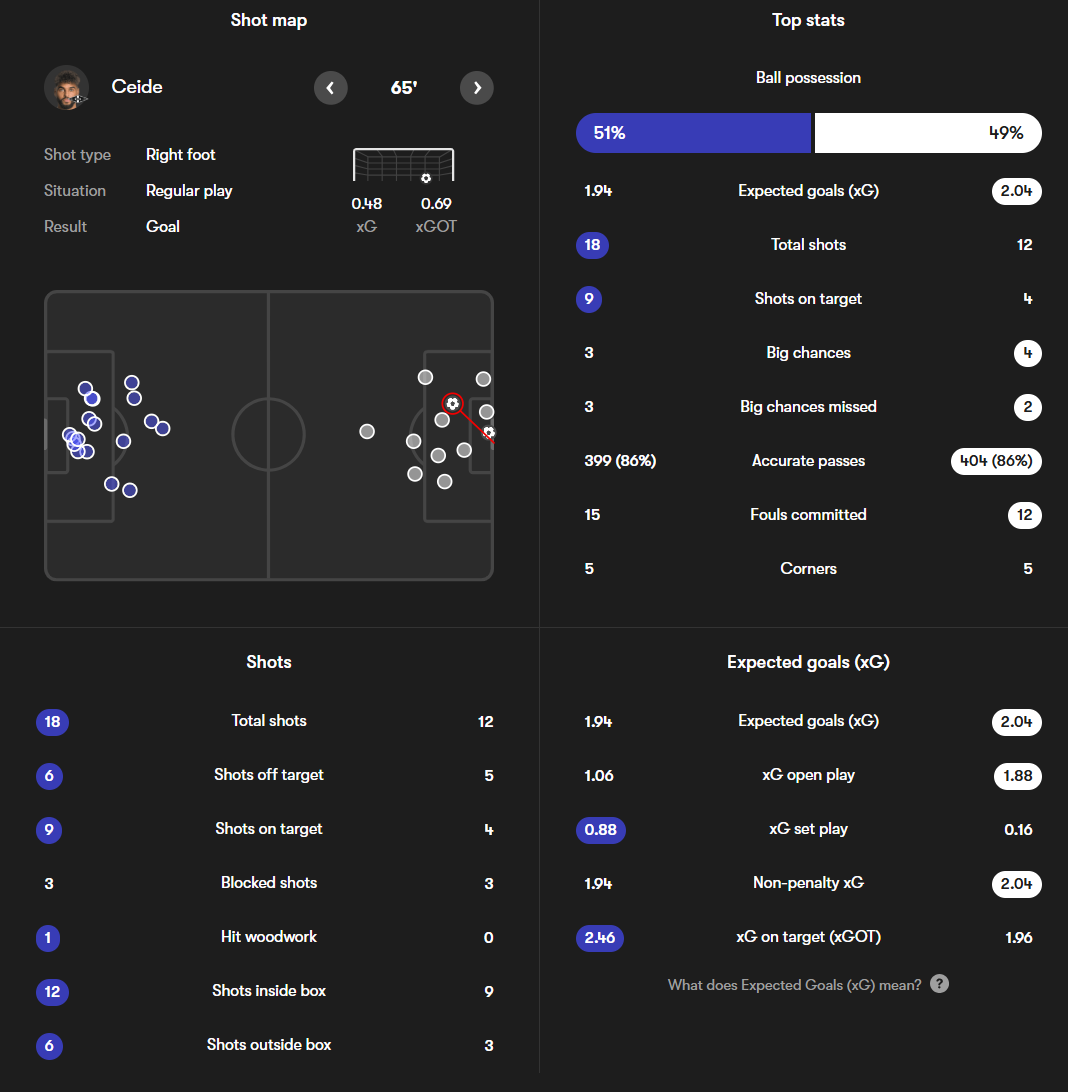
\includegraphics[width=0.5\linewidth]{figures/fotmob_rbk.png}
    \caption{Commercially available stats from a football game. Retrieved from FotMob\cite{fotmob_game}.}
    \label{fig:fotmob_stats}
\end{figure}

\begin{itemize}
    \item Event data: manually or commercially annotated discrete occurrences (passes, shots, corners).
    \begin{itemize}
        \item \acrfull{xg}: estimates shot quality using spatial and contextual features with XGBoost trained on large historic datasets \cite{mead_xg_2023}.
        \item Set pieces (corners, free kicks): naturally bounded events suitable for end-to-end predictive models.
        \item \autoref{fig:fotmob_stats} shows a selection of commercially available statistics. 
    \end{itemize}
    \item Tracking data: high-frequency player trajectories from GPS vests or manual optical systems.
    \begin{itemize}
        \item Physical metrics: distance covered, top speed, accelerations for workload monitoring and injury risk assessment \cite{hennessy_gps_tracker_2018}.
    \end{itemize}
\end{itemize}

\textcite{wang_tactic_ai_2024} applies deep graph neural networks to corners, a discrete sub-event of play. They deliver strong predictive and generalizable performance and have helped Liverpool FC succeed. 

\improvement{mention other datasets}
\improvement{move datasets used to method}
\unsure{maybe just a bullet list of existing sets}
\section{Datasets}
\label{sec:datasets}

\textcite{survey_of_survey} present comprehensive tables of sports action datasets. \textcite{seweryn_survey_2023} detail football‐specific collections.

\subsection{SoccerNet}

\textcite{deliege_soccernet-v2_dataset_2021} introduce SoccerNet-V2, offering 500 match recordings annotated with 17 football events action spotting.

In 2024 \textcite{deliege_soccernet-v2_dataset_2021} released 7 new games annotated with 12 ball events and team annotation. There are about 6 times the events in these 7 videos per video compared to the original 500. 

\subsection{UCF101}
UCF101 \cite{dataset:UCF101} comprises 13 320 YouTube clips spanning 101 human action categories. It serves as a standard benchmark for trimmed action recognition.

\subsection{THUMOS}
THUMOS \cite{dataset:thumos} includes over 13 000 temporally annotated instances from 20 action classes. It evaluates detection in untrimmed videos.

\subsection{HACS}
HACS \cite{dataset:hacs} comprises 1.55 million short clips across 200 action classes. It provides both trimmed classification clips and untrimmed temporal segments.

\subsection{ActivityNet}
The FineAction dataset \cite{dataset:fineaction} comprises 103\,K temporal instances across 106 fine-grained action categories, annotated in 17\,K untrimmed videos. It features dense, co-occurring action annotations and rich class diversity. FineAction offers a new benchmark for detailed temporal action localization.


\subsection{Kinetics}
Kinetics-400/600/700 \cite{dataset:kinetics} offers hundreds of thousands of 10-second clips labeled with 400–700 action classes. The clips are from YouTube.

\subsection{FineAction}
FineAction \cite{dataset:fineaction} provides 10 000+ short clips of soccer actions annotated at frame level with player bounding boxes. It enables fine-grained event spotting and player-centric analysis.



% \section{Datasets}
% \label{sec:datasets}

% \textcite
% A number of large‐scale video datasets have been developed to advance action recognition research. \textcite{survey_of_survey} provide comprehensive overviews of available sports‐related action datasets (see their Tables 4 & 5), while Seweryn et al.~\cite{seweryn_survey_2023} focus specifically on football‐centric collections. Below we summarize the main datasets examined in this thesis, ordered by their relevance and scale.


% \subsection{SoccerNet-V2}
% \label{ssec:soccernet}

% The SoccerNet-V2 dataset \cite{deliege_soccernet-v2_dataset_2021} contains video recordings of 7 professional football matches with fine-grained annotations for 12 action classes. It provides:
% \begin{itemize}
%     \item 7 full matches (90 min each) at 25 fps.
%     \item Time-stamped action labels for spotting tasks.
%     \item Team annotations for each event.
%     \item Publicly accessible via HuggingFace\footnote{\url{https://huggingface.co/datasets/SoccerNet/SN-BAS-2025}}.
%     \item The twelve football event classes:
%         \begin{center}
%             \begin{tabular}{llll}
%                 Pass & Drive & Header & High Pass \\
%                 Out & Cross & Throw In & Shot \\
%                 Ball Player Block & Player Successful Tackle & Free Kick & Goal
%             \end{tabular}
%         \end{center}
%     \item An action approximately every 3 seconds. 
% \end{itemize}

% The original SoccerNet dataset contains the recording of 500 games with 17 action classes. 


% \subsection{THUMOS'14}
% \label{ssec:thumos}

% The THUMOS'14 dataset \cite{dataset:thumos} comprises:
% \begin{itemize}
%     \item 20 action classes in sports and daily activities.
%     \item 213 untrimmed videos for temporal detection.
%     \item Predefined train/val/test splits for benchmarking.
% \end{itemize}

\section{Deep Learning} \improvement{Write this at a higher level?}
\label{sec:deep_learning}

Deep learning comprises multilayer neural networks that automatically learn hierarchical data representations. By contrast, classical methods rely on handcrafted features; deep architectures instead discover interesting patterns from raw inputs. They stack linear transformations and non-linear activations to extract meaningful features at each layer \cite{lecun_deep_learning_2015}. 
Early layers capture low-level primitives, while deeper layers combine these primitives into high-level concepts. Model training uses backpropagation to compute loss gradients with respect to millions of parameters. \unsure{to cv related, the second part?}

\subsection{Forward pass}
For a network with two hidden layers, the forward pass can be written as:
\begin{align}
z^{(1)} &= W^{(1)} x + b^{(1)}, & y^{(1)} &= f\bigl(z^{(1)}\bigr), \\
z^{(2)} &= W^{(2)} y^{(1)} + b^{(2)}, & y^{(2)} &= f\bigl(z^{(2)}\bigr), \\
z^{(3)} &= W^{(3)} y^{(2)} + b^{(3)}, & \hat{y} &= g\bigl(z^{(3)}\bigr).
\end{align}
Here, \(x\in\mathbb{R}^d\) is the input, \(W^{(l)},b^{(l)}\) are weights and biases at layer \(l\), \(f(.)\) is an activation function (e.g. ReLU). Figure~\ref{fig:forward_pass} illustrates these computations. In the case of a classification task, \(g\) is the output activation (e.g. softmax) and \(\hat{y}\) is the predicted class.

\begin{figure}[ht]
    \centering 
    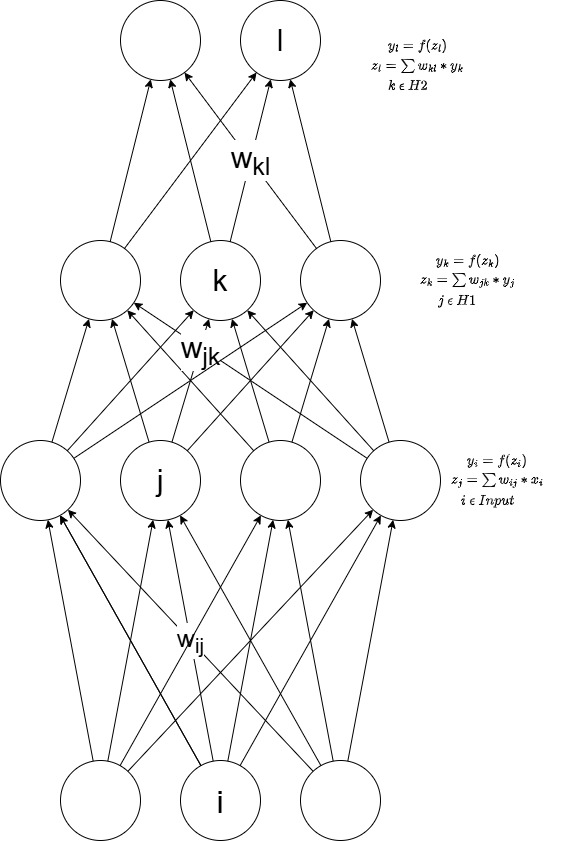
\includegraphics[width=0.6\linewidth]{figures/neural_net.jpg}
    \caption{Feedforward pass of a neural network with two hidden layers.} 
    \label{fig:forward_pass}
\end{figure}

\subsection{Backward pass}
Training minimizes a loss \(E(\hat y, y^\star)\), using e.g. cross-entropy. Gradients are computed via the chain rule:
\begin{align}
\delta^{(3)} &= \frac{\partial E}{\partial z^{(3)}}
= \frac{\partial E}{\partial \hat y}\odot g'\bigl(z^{(3)}\bigr),\\
\delta^{(l)} &= \frac{\partial E}{\partial z^{(l)}}
= \bigl(W^{(l+1)\top}\delta^{(l+1)}\bigr)\odot f'\bigl(z^{(l)}\bigr),
\quad l=2,1.
\end{align}
Weight and bias gradients follow:
\begin{align}
\nabla_{W^{(l)}}E &= \delta^{(l)}\,y^{(l-1)\top}, &
\nabla_{b^{(l)}}E &= \delta^{(l)},
\end{align}
with \(y^{(0)}\equiv x\). Figure~\ref{fig:backward_pass} shows the backpropagation flow.

\begin{figure}[ht]
    \centering
    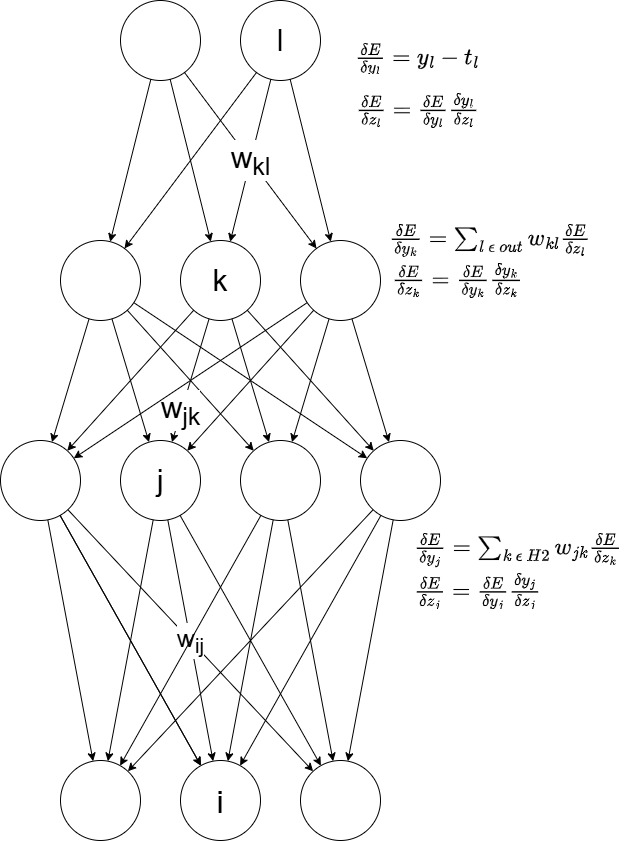
\includegraphics[width=0.6\linewidth]{figures/neural_net_back_prop.jpg}
    \caption{The equations that compute the backward pass.} 
    \label{fig:backward_pass}
\end{figure}

\subsection{Optimization}
Parameters are updated with stochastic gradient descent (SGD) or adaptive variants (Adam, RMSprop). For learning rate \(\eta\),
\[
W^{(l)} \leftarrow W^{(l)} - \eta\,\nabla_{W^{(l)}}E,
\quad
b^{(l)} \leftarrow b^{(l)} - \eta\,\nabla_{b^{(l)}}E.
\]
Regularization techniques such as weight decay, dropout and batch normalization further improve generalization and training stability \cite{ioffe_batch_2015}.

\subsection{Convolutions}
\improvement{I never alter formulas, is it necessary to explain them then} 

Convolutions learn small filters that slide over the input to detect local features in space (and time). Each filter is a small tensor of weights that computes a weighted sum plus a bias at every position. By sharing the same weights across all locations, convolutions capture patterns such as edges, textures, or motion.  

In the most basic scenario, when there is a layer with input dimensions of \( (N, C_{in}, H, W)\) and output dimensions of \( (N, C_{out}, H_{out}, W_{out})\), the output can be accurately described as follows:

\[out(N_i, C_{out_j}=bias(C_{out_j})+\sum_{k=0}^{C_{in}-1}weight(C_{out_j},k)\star input(N_i,k)\]

In this expression, the symbol \(\star\) represents the valid 2D cross-correlation operation. Here, \textit{\textbf{N}} refers to the batch size, \textit{\textbf{C}} indicates the number of channels, \textit{\textbf{H}} represents the height of the input planes measured in pixels, and \textit{\textbf{W}} denotes the width measured in pixels\cite{pytorch_conv2d}. 

Key components:
\begin{itemize}
    \item \textbf{Stride}, \textbf{padding}, and \textbf{dilation} control the receptive field and output resolution.
    \item \textbf{Pooling} (max or average) reduces spatial dimensions and enforces translational invariance.
    \item \textbf{Batch normalization} stabilizes learning by normalizing activations per mini-batch.
    \item Non-linear activations (ReLU, Leaky-ReLU, etc.). 
\end{itemize}

\begin{figure}
    \centering
    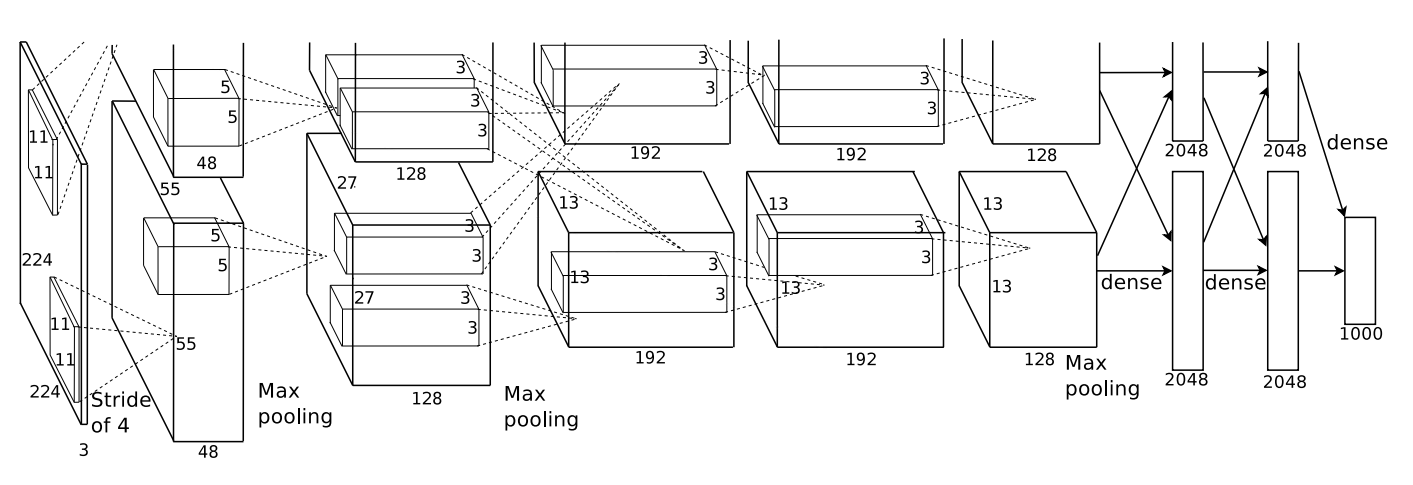
\includegraphics[width=1\linewidth]{figures/alexnet.png}
    \caption{An illustration of the architecture of AlexNet. One GPU runs the layer-parts at the top of the figure while the other runs the layer-parts at the bottom. The figure and caption is Figure 2 in the released paper by \textcite{krizhevsky_alexnet}.}
    \label{fig:alexnet}
\end{figure}

Stacking multiple convolution-activation-pooling blocks builds hierarchical feature representations, from edges and textures in early layers to object parts in deeper layers \cite{lecun_deep_learning_2015}. \autoref{fig:alexnet} shows how \textcite{krizhevsky_alexnet} designed AlexNet in 2012 with alternating convolution and pooling layers. Residual connections \cite{he_deep_residual_2015} further ease training in very deep networks by learning residual mappings. An example of a residual block is shown in \autoref{fig:res_connection}. Architectures such as Inception \cite{szegedy_going_2014}, MobileNet (depthwise separable convolution) \cite{howard_mobilenets_2017} and EfficientNet (compound scaling) \cite{tan_efficientnet_2020} optimize accuracy-efficiency trade-offs in image tasks. 

\begin{figure}
    \centering
    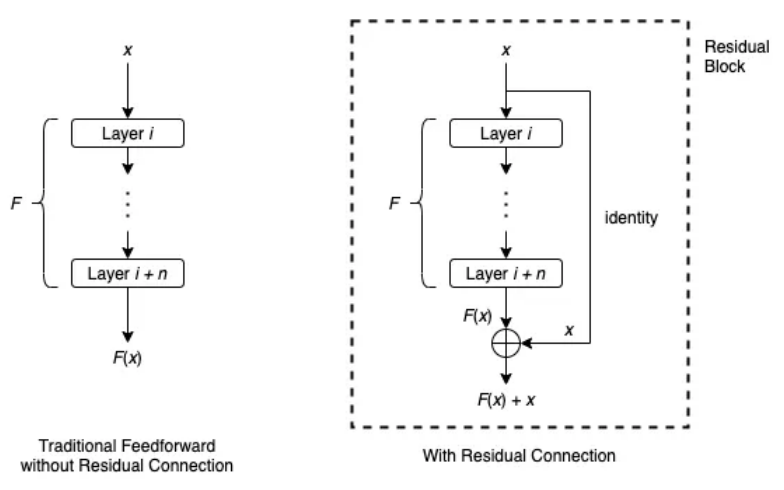
\includegraphics[width=0.5\linewidth]{figures/res_connection.png} 
    \caption{Residual block. Created by \textcite{wong_what_is_residual_2022}. }
    \label{fig:res_connection}
\end{figure}

In the video domain, spatiotemporal convolutions extend the same principles along time.  Early 3D \acrshort{cnn}s \cite{tran_learning_2015} apply cubic kernels to capture motion, but suffer from high computational cost.  The (2+1)D decomposition \cite{tran_2_plus_1_convolution} splits 3D kernels into separate spatial and temporal convolutions, improving the optimization.  The Inflated 3D \acrshort{cnn} (I3D) \cite{carreira_2017_i3d_quo_vadis} “inflates” pretrained 2D filters into the time dimension. This creates a balance between efficiency and representation.

Further advances address long-range temporal modeling:
\begin{itemize}
    \item SlowFast networks \cite{feichtenhofer_slowfast_2019} use a dual-pathway: a \emph{Slow} branch at low frame rate for semantics and a \emph{Fast} branch at high frame rate for motion.  
    \item Temporal Shift Module (TSM) \cite{lin_temporal_shift_2019} achieves temporal modeling by shifting feature channels across frames with zero extra parameters.  
    \item X3D \cite{feichtenhofer_x3d_2020} systematically expands 2D image models into efficient, scalable 3D architectures by progressive width, depth and resolution scaling.
\end{itemize}

Despite their locality bias, \acrshort{cnn}-based video models remain foundational building blocks in modern action-recognition frameworks, often combined with non-local blocks or attention to capture global spatiotemporal dependencies.
\info{another paragraph with a different approach is below} 


\subsection{Recurrent Neural Nets}

\acrfull{rnn} are a class of deep learning models designed to handle sequential data. \acrshort{rnn}s keep a memory of previous inputs. Unlike tradtional feedforward networks, for example \acrshort{cnn}s and neural nets, \acrshort{rnn}s use feedback loops that allows information to exist over multiple time steps. \unsure{Do I say the same sentence twice here?} This makes \acrshort{rnn}s useful for tasks requiring temporal dependencies, such as natural language processing, speech recognition and time-series forecasting\cite{ibm_rnn_2025}. In the context of \acrfull{cv}, \acrshort{rnn}s have been applied for applications such as image captioning or video analysis. \unsure{Is it better to write in present?}

Standard \acrshort{rnn}s suffer from the vanishing gradient problem. The issue is due to repeated multiplication of small gradient values during backpropagation through time. This leads to diminishing updates in early layers. \acrfull{lstm} is one solution to this problem \cite{bhogal_human_2023, kumar_human_2023, mahaseni_spotting_2021}.The other widespread solution is the \acrfull{gru} \cite{giveki_human_2024,li_oarnet_2024,yu_i3d_2023}. 

\acrlong{lstm} introduce memory cells. The cells are equipped with input, forget and output gates. \acrshort{lstm}s come with increased efficiency and increased complexity. On small datasets \acrshort{lstm}s are prone to overfitting. 

\acrlong{gru}s use a reset gate and an update gate to maintain or discard information. It has fewer parameters than an \acrshort{lstm}, which makes them more computationally efficient while addressing the vanishing gradient problem. \acrshort{gru} are particularly attractive in scenarios with limited resources. 

\acrshort{rnn}-based architectures are used in video analysis models to capture temporal dependencies, like \textcite{bhogal_human_2023}. Although a historically popular resource for sequential data processing, transformer models have led to a decline in their usage. However, they remain relevant in contexts where step-by-step recurrence and memory provide distinct advantages\cite{ibm_rnn_2025}.

\subsubsection{Bi-Directional Layers}
\label{ssec:bi_directional_layers}

Bi-directional recurrent layers combine two parallel LSTM networks to capture both past and future context in a sequence \cite{radhakrishnan_bi_lstm_2023, bhogal_human_2023}. One LSTM processes the input in its original order (forward pass), while the other processes it in reverse (backward pass). At each time step \(t\), the hidden states from both directions are concatenated to form a richer representation of the data:

\[
h_t = \bigl[\,\overrightarrow{h}_t;\,\overleftarrow{h}_t\bigr].
\]

In the context of football analytics, this approach is useful because events (e.g.\ goals, passes) often depend on both preceding and succeeding actions on the field. By integrating information from before and after a given frame, bi-directional layers can improve the accuracy of sequence predictions. The main trade-off is that they require roughly twice the number of parameters and incur longer training and inference times compared to unidirectional models.


\subsection{Vision Transformers}
\label{ssec:vision_transformers}

\acrfull{vit} adapt the transformer architecture \cite{vaswani_attention_2017} \change{Does transformers by themselves deserve a section?} to images by splitting each image into $P\times P$ patches, projecting them to $D$-dimensional embeddings, and adding positional encodings \cite{dosovitskiy_image_transformer_2021}. Given an image of size $H\times W$, one obtains
\[
\mathbf{x}_0 = [x_{\text{cls}};\,z_1,\dots,z_N] + E_{\text{pos}},
\]
$x_{\text{cls}}$ is a learnable classification token, and $E_{\text{pos}}\in\mathbb{R}^{(N+1)\times D}$ are positional embeddings, where $N=(H/P)\,(W/P)$,. The sequence is processed by $L$ identical blocks of multi-head self-attention (MSA) and feed-forward networks (FFN)\cite{dosovitskiy_image_transformer_2021}:
\begin{align*}
y^l &= \mathrm{MSA}\bigl(\mathrm{LN}(x^{l-1})\bigr) + x^{l-1},\\
x^l &= \mathrm{FFN}\bigl(\mathrm{LN}(y^l)\bigr) + y^l,\quad l=1,\dots,L.
\end{align*}

TimeSformer \cite{bertasius_timesformer_2021} extends ViT to video by factorizing self-attention into separate spatial and temporal modules, reducing complexity from $\mathcal{O}\bigl((TN)^2\bigr)$ to $\mathcal{O}(T^2N + N^2T)$. Formally, with tokens $z_{t,n}$ for frame $t$ and patch $n$,
\[
\mathrm{Attn}(Z)
= \mathrm{Softmax}\!\bigl(Q_sK_s^\top/\sqrt{D}\bigr)V_s
+ \mathrm{Softmax}\!\bigl(Q_tK_t^\top/\sqrt{D}\bigr)V_t.
\]

VViT \cite{arnab_vvit_2021} further improves video classification by combining factorized attention with multi-scale patch embeddings, achieving state-of-the-art results on multiple benchmarks.


Limitations of vision transformers include:
\begin{itemize}

    \item High data requirements—performance degrades on small or specialized datasets.  
    \item Computational cost—quadratic scaling with sequence length impacts memory and runtime.  
    \item Model complexity—large parameter counts increase overfitting risk \cite{lee_enhancing_mamba_s6_2024}.
\end{itemize}


\subsubsection{META Segment Anything Model 2}
\label{ssec:meta_sam2}

The Segment Anything Model (SAM) was first introduced by Kirillov et al.\ \cite{kirillov_segment_2023} in 2023 as a promptable, foundation segmentation model.  Its core design splits the task into three components:
\begin{itemize}
    \item \textbf{Image Encoder:} A vision transformer (ViT) pretrained on masked autoencoding, which produces dense feature maps for any input image.
    \item \textbf{Prompt Encoder:} A lightweight module that maps interactive prompts (points, bounding boxes or free-form masks) into positional embeddings.
    \item \textbf{Mask Decoder:} A small transformer that fuses image and prompt embeddings to output segmentation masks at multiple scales.
\end{itemize}
SAM was trained on the enormous SA-1B dataset (over 11 M images and 1.1 B masks) in a semi-automated pipeline, yielding strong zero-shot performance across diverse domains without any finetuning.

Building on this success, Ravi et al.\ \cite{ravi_sam_nodate} proposed \emph{SAM-2} (sometimes called Video \acrshort{sam}), which extends \acrshort{sam} to sequential video data via a \emph{memory-augmented attention} mechanism:
\begin{itemize}
    \item \textbf{Frame-wise Encoding:} Each video frame is encoded by the same ViT backbone used in image \acrshort{sam}.
    \item \textbf{Memory Attention:} A cross-frame attention layer that retains a compact set of “memory tokens” summarizing past masks, enabling consistent tracking of object masks over time.
    \item \textbf{Interactive Prompts in Video:} Mouse clicks and bounding-box prompts can be applied on any frame, and propagated forward or backward via the memory bank.
\end{itemize}
The authors also released SA-V, a large video-segmentation dataset with millions of frame-mask pairs, demonstrating that \acrshort{sam}-2 achieves near real-time inference (15-30 fps) and high temporal consistency on common benchmarks.

Together, the original \acrshort{sam} and its video-centric successor exemplify a new paradigm in segmentation: a single, promtable\unsure{promtable or promtable?} transformer that can be deployed off-the-shelf, adapted to novel objects or domains with minimal human guidance, and extended from static images to dynamic scenes. 

\improvement{To increase readability I this section needs more figures, not only here}
\subsection{State-Space Models}
\label{ssec:state_space_models}
\improvement{Temporal Modeling Techniques” (RNN, TCN, TSN, Transformers) can be summarized in Background—only the variants you actually implement/test (e.g. your MAMBA variant, TSN baseline) get full detail in Methods}
% \acrfull{ssm} offer a continuous-time representation of sequential data via a latent state \(h(t)\in\mathbb{R}^N\):
% \begin{align}
%     \frac{\mathrm{d}h(t)}{\mathrm{d}t} &= A\,h(t) + B\,x(t),  \label{eq:ssm_continuous1}\\
%     y(t) &= C\,h(t),                                    \label{eq:ssm_continuous2}
% \end{align}
% where \(x(t)\in\mathbb{R}^d\) is the input, \(y(t)\in\mathbb{R}^m\) the output, and \(A\in\mathbb{R}^{N\times N}, B\in\mathbb{R}^{N\times d}, C\in\mathbb{R}^{m\times N}\) are learned parameters.  Discretizing these equations with step size \(\Delta\) yields
% \begin{align}
%     \bar A &= \exp(\Delta\,A), 
%     & 
%     \bar B &= \bigl(\exp(\Delta\,A)-I\bigr)A^{-1}B,\\
%     h_k &= \bar A\,h_{k-1} + \bar B\,x_k, 
%     &
%     y_k &= C\,h_k,
%     \quad k=1,2,\dots
% \end{align}
% \unsure{Do I have to reference equations in the same way figures must be referenced in a text}
% VideoMamba \cite{li_videomamba_2024} builds on this framework with a \emph{Selective Scan} (\acrshort{s6}) core.  Its parameters \((\Delta, A,B,C)\) control:
% \begin{itemize}
%     \item \(\Delta\): temporal resolution of the recurrence,
%     \item \(A\): continuous dynamics matrix,
%     \item \(B,C\): input and output mappings.
% \end{itemize}

% By preserving a compact hidden state, Mamba approximates long-range dependencies akin to self-attention but with only \(\mathcal{O}(L)\) time/memory cost rather than \(\mathcal{O}(L^2)\).  

VideoMAMBA extends \acrshort{s6} to spatiotemporal video features: each frame is first embedded (e.g.\ via convolutional or patch-based encoders) into \(x_k\), then processed through the discrete SSM along the temporal dimension.  Prior studies \cite{lee_enhancing_mamba_s6_2024, li_videomamba_2024} report that VideoMAMBA matches transformer-based action recognition on common benchmarks while reducing inference overhead.

This thesis applies the VideoMAMBA suite to a newly collected football video dataset to evaluate its event-spotting performance (see Chapter~\ref{chap:experiments}). The results demonstrate that VideoMAMBA not only achieves competitive accuracy but also delivers substantial gains in inference speed and memory efficiency, confirming the practicality of state-space models for large-scale video analytics. \unsure{Remove this paragraph? Move to intro?}


\subsection{Training Strategies}
\label{ssec:training_stratergies}
\improvement{“Training Strategies” (supervised vs. unsupervised) reads like a textbook. Focus only on the strategies you actually use (masked AE + distillation).}
\subsubsection{Learning Paradigms}
A model must be trained on domain-specific data to achieve its full potential. Training algorithms for artificial neural networks (ANNs) can be broadly grouped into four categories: supervised learning, unsupervised learning, self-supervised learning, and reinforcement learning. This thesis \improvement{Replace this thesis } focuses on supervised and unsupervised learning, which are detailed below.

\paragraph{Supervised Learning}
In supervised learning, models are trained on labeled data comprising input-output pairs \((x_i, y_i)\). The objective is to learn a mapping that generalizes to unseen data. In this thesis\improvement{"this thesis"}, supervised labels include bounding-box coordinates of players and the ball in football match images, and the model is tasked with detecting these objects in new footage. Gradient descent optimizes the parameters \(\theta\) by minimizing a loss function \(J(y_i, \hat y_i)\):  
\[
\theta \leftarrow \theta - \eta \,\nabla_{\theta}J\bigl(y_i,\hat y_i\bigr),
\]
where \(\eta\) is the learning rate. Updates continue over the dataset until a stopping condition is met (e.g., maximum epochs, target loss, or early stopping).

\paragraph{Unsupervised Learning}
Unsupervised learning discovers structure from unlabeled data without explicit targets. Common tasks include clustering, association rule learning, and dimensionality reduction. \unsure{should I write just about supervised learning?}

\subsubsection{Masking}

In an encoder-decoder masking setup, the input video frames are first tokenized into spatio-temporal patches. A binary mask tensor \(M\in\{0,1\}^{T\times H\times W}\) with masking ratio \(r\) is generated, where
\[
\sum_{t,h,w} M_{t,h,w} = r\,T\,H\,W.
\]
The visible patches \(x_\text{vis}\) are obtained by
\[
x_\text{vis} = x \,\odot\,(1 - M)\,,
\]
and fed into a lightweight transformer encoder \(E\). The decoder \(D\) takes the encoder output plus positional embeddings and mask tokens, and attempts to reconstruct the original video:
\[
\hat{x} = D\bigl(E(x_\text{vis}),\,\text{mask\_tokens}\bigr).
\]
The model is trained to minimize the reconstruction loss only over masked positions:
\[
\mathcal{L} \;=\; \bigl\lVert\,M \,\odot\,(x - \hat{x})\bigr\rVert_2^2.
\]
Different masking strategies can be used:
\begin{itemize}
    \item Random tube masking: mask entire temporal tubes to encourage long-range dynamics learning.
    \item Block spatial masking: mask contiguous patches in each frame.
    \item Uniform patch masking: randomly mask individual patches across space and time.
\end{itemize}
High masking ratios (e.g.\ 75-90\%) force the encoder to capture global context, while the decoder reconstructs fine-grained details from a compact latent code. This approach underlies VideoMAE and similar masked autoencoder variants for self-supervised video representation learning.


Encoding and masking techniques are used with video data because of their inherent large size. Encoding encapsulates the process of compressing video files to reduce size while keeping a satisfactory quality. Video masking is the technique used to discard uninteresting regions and patches to focus on more meaningful features. This motivates the model to learn meaningful representations, rather than predicting based on redundant data \cite{tong_videomae_2022}. The most prominent masking variant used on \acrshort{sota} benchmarks on Papers with Code' in the category \textit{Action Recognition}\footnote{\url{https://paperswithcode.com/task/action-recognition-in-videos}} is the VideoMAE V2 \cite{wang_videomae_2023} and its highly related InternVideo2 \cite{wang_internvideo2_2024}. 

\textcite{tong_videomae_2022} address the problem of training video transformers from scratch. The aim is to use self-supervised learning to capture meaningful representations which enables the model to decode data into the original representations. The contributions of the masked autoencoder \cite{tong_videomae_2022} are the ability to train \acrshort{vit}s on smaller datasets. VideoMAE \cite{tong_videomae_2022} also tackle the problems of temporal relations in video-data and suggests a high masking ratio. VideoMAE-V2 \cite{wang_videomae_2023} improves the VideoMAE-models training time. It is still a very computationally expensive approach. 


\subsubsection{Knowledge Distillation}
\label{sssec:knowledge_distillation}

Knowledge distillation trains a compact \emph{student} model to mimic a larger, pre-trained \emph{teacher} model \cite{denize_comedian_2024, li_videomamba_2024, bose_soccerkdnet_2023}. By matching the teacher's softened output distribution (using a temperature-scaled softmax), the student can achieve similar accuracy with far fewer parameters. This reduction in size and computation is particularly valuable for video models with high inference cost.

However, distillation also has limitations:
\begin{itemize}
    \item A weak teacher leads to a weak student—distillation cannot exceed the teacher's performance.
    \item Training both teacher and student increases total computational cost.
    \item Some fine-grained knowledge may not transfer fully, which can hurt the student's generalization on new data.
\end{itemize}


\section{Computer Vision} 
\label{sec:computer_vision}

\acrfull{cv} is a subset of machine learning that focuses on letting computers interpret and understand digital images and videos. The aim of \acrlong{cv} is to enable computers to see. Some tasks relating to computer vision, extracted from Papers with Code\footnote{\url{https://paperswithcode.com/datasets}}, are Action Recognition, Object Detection, Semantic Segmentation, Classification and Question Answering. 

\subsection{Hand-Crafted methods}

\begin{figure}
    \centering
    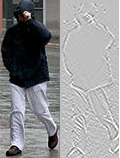
\includegraphics[width=0.5\linewidth]{figures/Pedestrian_gradient.jpg}
    \caption{An image of a pedestrian and his gradient calculated by \acrshort{hog}.}
    \label{fig:pedestrian_gradient}
\end{figure}

Before the rise of deep learning, early computer vision research predominantly relied on manually engineered features. One of the influential approaches was the \acrfull{hog} introduced by \textcite{dalal_histogram_of_gradients}. This method was designed to detect humans in static images by partitioning an image into small regions and computing gradient directions within each patch, ultimately assembling these measurements into a descriptive feature vector. \autoref{fig:pedestrian_gradient} visualizes the gradient vectors. In a similar fashion, action recognition in videos was addressed through the Histogram of Flow\cite{dalal_histogram_of_flow}. This technique extends the \acrshort{hog} concept by calculating gradient descriptors at each frame, capturing motion information through the analysis of optical flows. Then combining these per-frame descriptors into a representation that encapsulates temporal dynamics. \unsure{The HOG image is from Wikipedia, but they do not provide any source for it.}

Despite the innovation these approaches brought to early computer vision, their limitations soon became apparent. The reliance on accurate hand-crafted features often led to challenges in scaling to complex scenarios and achieving generalization. With the arrival of deep learning and its ability to learn hierarchical, data-driven representations, these manual methods have been largely outpaced. 

\subsection{Skeleton and Posture Estimation}
\label{ssec:skeleton_posture_estimation}

Skeleton and posture estimation techniques recover 2D or 3D joint coordinates from video frames to model player kinematics and pose dynamics \cite{elaoud_skeleton-based_2020, wang_skeleton_two-stream_2023, reilly__skeleton_just_pi_2023}. Common pipelines include:
\begin{itemize}
    \item Top-down methods: detect each player via bounding boxes, then apply a single-person pose estimator.
    \item Bottom-up methods: predict all joint candidates first and group them into skeletons.
    \item Graph-based models: use spatial-temporal graph convolutional networks (ST-GCN) to capture joint correlations over time\cite{yan_spatial_temporal_graph_convolutional_2018}.
\end{itemize}
These approaches enable extraction of features such as joint angles, stride length and posture transitions for performance analysis and injury risk assessment. In football scenarios, however, they face:
\begin{itemize}
    \item Severe occlusions and player overlaps in crowded penalty areas.
    \item Varying camera angles, resolutions and lens distortions.
    \item Fast motions causing motion blur and tracking drift\cite{survey_of_survey}.
\end{itemize} 


\section{Problem Formulation}
\label{sec:problem_formulation}
\improvement{move to motivation/intro/together with rq}
\improvement{title change}

\subsection{Action Spotting vs.\ Action Localization}
Action spotting casts each event as a single instant in time, reducing annotation to one timestamp per occurrence. By contrast, action localization requires predicting both start and end times for each action interval and is typically evaluated with temporal \acrfull{iou} metrics. Spotting simplifies supervision and evaluation (via tolerance windows around true timestamps), but it also challenges models to resolve events occurring in close temporal proximity without relying on segment boundaries.

\subsection{Temporal vs.\ Spatiotemporal Tasks}
Temporal event spotting focuses solely on “when” an action occurs, using global frame or clip‐level features. Spatiotemporal tasks, in comparison, demand joint localization in time and space (e.g.\ frame‐level bounding boxes). The SoccerNet challenge remains in the temporal domain.

\subsection{Notation and Task Definition}
Let
\begin{itemize}
  \item $V=\{x_t\}_{t=1}^T$ be an input video of $T$ frames,
  \item $\mathcal{C}=\{1,\dots,12\}$ the set of action classes,
  \item $\mathcal{Y}=\{(t_i,c_i)\}_{i=1}^N$ the ground-truth annotations (timestamp $t_i$, class $c_i$),
  \item $\hat{\mathcal{Y}}=\{(\hat t_j,\hat c_j,\hat s_j)\}_{j=1}^M$ the model's predicted timestamps, classes and confidence scores.
\end{itemize}
A prediction $(\hat t_j,\hat c_j)$ is correct if $\hat c_j=c_i$ and $|\hat t_j - t_i|\le\Delta$, where $\Delta$ is a fixed tolerance window (e.g.\ 1 s). Performance is measured by \acrfull{map} over all classes under the chosen $\Delta$.
\section{Temporal Modeling Techniques}\unsure{Should I remove this section}
\label{sec:temporal_models}

Temporal modeling techniques aim to capture motion and long-range dependencies across video frames. Common approaches include: \unsure{is this redundant}

\paragraph{\acrfull{rnn}}  
LSTM and GRU cells process a sequence of frame features \(x_t\in\mathbb{R}^d\) by carrying a hidden state \(h_t\):
\[
h_t = \mathrm{LSTM}(x_t,\,h_{t-1}), 
\qquad
\hat y_t = \mathrm{softmax}(W_o\,h_t + b_o).
\]
Gating mechanisms alleviate vanishing gradients but incur computation overhead.

\paragraph{Temporal Convolutional Networks (TCNs)}  
Dilated 1D convolutions aggregate information over multiple time steps in parallel:
\[
y_t = \sum_{k=0}^{K-1} w_k\,x_{t - d\,k} + b,
\]
where \(d\) is the dilation factor and \(K\) the kernel size. TCNs achieve large receptive fields with fewer layers.

\paragraph{Self-Attention Models}  
Transformers treat each frame's embedding as a token and apply multi-head attention:
\[
\mathrm{Attn}(Q,K,V) = \mathrm{softmax}\bigl(QK^\top/\sqrt{D}\bigr)\,V.
\]
They capture global context at quadratic cost in sequence length.

\subsubsection{Temporal Segment Networks (TSN)}  
TSN splits a video into \(S\) segments, randomly samples one snippet per segment, extracts per-snippet features via a 2D \acrshort{cnn}, and fuses them with a consensus function (e.g.\ average pooling):
\[
F = \frac{1}{S}\sum_{s=1}^{S}f\bigl(\mathrm{CNN}(x_s)\bigr).
\]
By sparsely sampling over long videos, TSN balances efficiency and temporal coverage.

\section{Evaluation Metrics and Protocols}
\label{sec:evaluation}

\subsection{Spotting-Level Metrics}
\subsubsection{Mean Average Precision (mAP)}
Each predicted timestamp is treated with $\hat t_j$ with class $\hat c_j$ as a detection. A true positive occurs if there exists a ground-truth event $(t_i,c_i)$ such that $\hat c_j = c_i$ and $|\hat t_j - t_i|\le\Delta$, where $\Delta$ is a fixed tolerance window (e.g.\ 1\,s). All unmatched predictions are false positives, and missed ground-truth events are false negatives. We compute precision-recall curves per class and report
\[
\mathrm{AP}_c = \int_{0}^{1} p_c(r)\,\mathrm{d}r,\quad
\mathrm{mAP} = \frac{1}{|\mathcal{C}|}\sum_{c\in\mathcal{C}}\mathrm{AP}_c.
\]

\subsubsection{Precision / Recall @ Tolerance}
In addition to mAP, we report precision and recall at fixed tolerance levels $\Delta\in\{0.5,1.0,2.0\}$\,s. This highlights the trade-off between temporal precision (small $\Delta$) and detection rate.

\subsection{Localization-Level Metrics}
\subsubsection{\acrfull{iou}}
For methods that predict temporal segments $[s_j,e_j]$, we measure overlap with ground-truth intervals $[t_i-\tfrac{\tau_i}{2},\,t_i+\tfrac{\tau_i}{2}]$ via
\[
\mathrm{IoU}([s_j,e_j],\,[g_s,g_e]) 
= \frac{|[s_j,e_j]\cap [g_s,g_e]|}{|[s_j,e_j]\cup [g_s,g_e]|}.
\]
A segment is correct if $\mathrm{IoU}\!\ge\theta$ and $\hat c_j=c_i$.

\subsubsection{mAP @ IoU Thresholds}
\acrshort{map} is computed as above, replacing the tolerance criterion $|\hat t_j - t_i|\le\Delta$ with $\mathrm{IoU}\ge\theta$ for $\theta\in\{0.3,0.5,0.7\}$. This compares single-timestamp spotting to full localization performance.

\subsection{Computational Metrics} 
\subsubsection{Inference Latency} 
Measure time lol. But we already know that MAMBA is faster \unsure{is this a necessary topic, to talk about how to measure time}
\todo{write if necessary}

\subsection{Metrics Correlation and Importance}

Hyperparameter correlation measures the linear relationship between a hyperparameter and a selected metric, such as validation loss. A high correlation implies that an increase or decrease in the hyperparameter value leads to a similar change in the metric. However, correlation alone does not capture second-order interactions or non-linear dependencies.

To address these limitations, importance metrics are derived using a tree-based model, specifically a **random forest**, trained on hyperparameters as inputs and the performance metric as the target output. Feature importance values from this model provide deeper insights into which hyperparameters significantly impact results. Unlike linear models, tree-based approaches are more robust to categorical data and non-normalized values.

\section{Related Work in Football Event Spotting}
\label{sec:fw_work}

COMEDIAN \cite{denize_comedian_2024} combines self-supervised learning and knowledge distillation to initialize a transformer for action-spotting on the SoccerNet-V2 dataset \cite{deliege_soccernet-v2_dataset_2021}. The contributions from Denize et al. are a three-step training pipeline and \acrshort{sota} performance. The first step is to use self-supervised pretraining on a spatial transformer. The second step is to initialize a temporal transformer by using knowledge distillation to enrich the spatial transformers output. The last step is the training on the relevant action spotting task, in this case the SoccerNet-V2 \cite{deliege_soccernet-v2_dataset_2021}.

T-DEED \cite{xarles_t-deed_2024} is a Temporal-Discriminability Enhancer Encoder-Decoder, which won the action spotting category of SoccerNet 2024 \cite{cioppa_soccernet_2024}. The temporal part refers to looking at different lengths of time in the video. Discriminability is making sure each frame of the video is distinct. Encoder-decoder refers to compressing and expanding the video information. The model utilizes \acrfull{sgp} to enhance its discriminability between tokens. This is useful because sports actions can appear similar. \todo{write more?}

In 2021 Gerats et al\cite{gerats_individual_same_task_2021} worked with a single static panorama camera for action-spotting and activity recognition. They use player snippets as model input. Inflated 3D \acrshort{cnn} is used to extract spatio-temporal features from the snippets. A graph attention network is used to analyze the relationship between players and their activities and actions.

\todo{add relevant articles from literature search}
\todo{internvideo 2}
\todo{rdfas6}
\improvement{Change \textit{"This thesis"} to something else.}
\improvement{Check pronouns}
\unsure{Check spelling}
\unsure{To move all related work to the end or keep them together with their section}
\improvement{what sections to move to the method part}
\improvement{A subsection about rdfa-s6}

\todo{General feedback • Prune repetitive definitions (RNN gating details, basic backprop) unless directly relevant.
• Group related items tightly: all masking/AEs under one “Self-Supervised Pretraining” heading; all sequence models under a single “Temporal Modeling” theme.
• Use neutral academic style: replace “this thesis” with “the present work” or “the proposed method.”
• Check figure placement: each major concept benefits from a schematic (e.g. pipeline, masking schedule, SSM recurrence).
• Spell-check and unify acronym expansions on first use; remove stray unsure{} and todo{} comments}

\improvement{write about parameter importance in wandb https://docs.wandb.ai/guides/app/features/panels/parameter-importance/}

\improvement{write about correlation?}
\chapter{Methodology} 
\label{chap:methodology}
This chapter describes the experimental setup used to evaluate the \acrfull{s6} model for temporal event spotting in football video. The section details computing infrastructure, data preprocessing and feature extraction pipeline, model architectures, training protocols, and evaluation metrics aligned with the research questions (\autoref{sec:research_questions}).


\section{Tools and Resources}
\label{sec:tools_and_resources}

\subsection{IDUN}
\label{ssec:idun}
Video processing pipelines demand substantial computational resources. To address this, I utilized the IDUN cluster\footnote{\url{https://www.hpc.ntnu.no/idun/}}. IDUN is a faculty-operated system at NTNU equipped with 234 NVIDIA GPU accelerators (as of April 24, 2024). Although IDUN is not NTNU’s central supercomputer, its nodes, featuring Tesla H100 and A100 GPUs, with up to 80 GB of RAM—provided the necessary throughput for feature extraction and model training. To mitigate occasional queuing delays and VRAM limitations, full-match videos were partitioned into fixed-duration clips and distributed workloads across multiple GPUs via data-parallel training.

Due to the high memory requirements of the \acrlong{tdeed} and software requirements of the \acrlong{s6} framework, all experiments were run on IDUN nodes equipped with modern NVIDIA GPUs. Attempts to train on GPUs with 16 GB of memory triggers out-of-memory errors on occasion with \acrshort{tdeed}. Moreover, MAMBA \acrshort{s6} requires certain CUDA versions and matching libraries, which older driver stacks do not support out of the box. To guarantee stable training and reproducible results, model development and evaluation to was restricted to nodes meeting these hardware and software requirements. 
% later was run on all types of GPU I have no reason how. 

% \subsection{draw.io}
% \label{ssec:draw.io}
% For the creation and maintenance of all schematic overviews—such as model architectures, data‐flow pipelines, and experimental workflows—we employed draw.io (diagrams.net). draw.io is an open-source, web-based diagramming tool that allows rapid assembly of vector‐based figures using a rich library of shapes, connectors and templates. Its native XML file format preserves editability and version history, facilitating collaborative revisions via version control, while export to PDF and SVG ensures high‐resolution inclusion in the thesis document. By standardizing figure style and layout across chapters, draw.io helped maintain visual consistency and improved the clarity of complex methodological and architectural descriptions.

\subsection{\acrfull{wandb}}
\label{ssec:wandb}
To streamline the management and reproducibility of the training experiments, I used the \acrlong{wandb} platform. Using \acrshort{wandb}’s Python client, hyperparameters are logged automatically. As is training and validation metrics, model checkpoints, and GPU utilization statistics. The centralized dashboard enabled real-time monitoring and direct comparison of concurrent runs. Crucially, \acrshort{wandb}’s automated hyperparameter sweep feature was used to conduct systematic searches over predefined parameter distributions. These sweeps coordinated parallel trials, performance metrics, and ranked configurations based on validation outcomes. By integrating \acrshort{wandb} into the workflow, it significantly enhanced the transparency, comparability, and reproducibility of the experimental pipeline.

\subsection{Bayesian Hyperparameter Search}

Bayesian optimization is a probabilistic approach to hyperparameter tuning that efficiently explores the search space by balancing **exploration** (trying new regions) and **exploitation** (focusing on promising regions). It builds a **surrogate model**, typically a **Gaussian Process**, to approximate the objective function and predict both the mean and variance of the function.

The optimization process follows these steps:
\begin{itemize}
    \item \textbf{Surrogate Model}: A probabilistic model estimates the objective function based on previous evaluations.
    \item \textbf{Acquisition Function}: Determines the next hyperparameter set to evaluate by optimizing a function such as **Expected Improvement (EI)** or **Upper Confidence Bound (UCB)**.
    \item \textbf{Evaluation and Update}: The chosen hyperparameters are tested, and the surrogate model is updated with new information.
    \item \textbf{Iteration}: The process repeats until convergence or a stopping criterion is met.
\end{itemize}

Bayesian optimization is particularly useful for tuning hyperparameters in deep learning models, where evaluating each configuration is computationally expensive. By leveraging probabilistic modeling, it efficiently identifies optimal hyperparameter values while minimizing unnecessary evaluations.

\subsection{Comparing Correlation and Importance}

While correlation identifies linear dependencies, importance accounts for complex interactions among multiple hyperparameters. This distinction helps researchers make informed decisions when designing hyperparameter search strategies. Bayesian optimization further enhances this process by intelligently selecting hyperparameters based on probabilistic predictions, leading to improved model performance and faster convergence.

\subsection{Anaconda and pip}
\label{ssec:conda_pip}
Python environments were managed using conda, but all packages—including CUDA-enabled PyTorch builds—were installed via pip to follow recent PyTorch recommendations favoring pip over conda for GPU support.

\section{Data Preprocessing \& Feature Extraction}
\label{sec:preprocessing}

Experiments are conducted on the SoccerNet-V2 dataset\cite{deliege_soccernet-v2_dataset_2021}. Videos are split into non-overlapping clips $V_k=\{x_t\}_{t=1}^{T_c}$ of fixed duration $T_c=60\!\times\!25$ frames (60\,s at 25\,fps). A 70-30 split and an 80-20 respectively for training and validation was used. The 80-20 split matches the official publication. 70-30 matches a PyTorch recommendation in the docs
\footnote{
\url{https://docs.pytorch.org/docs/stable/data.html}. 
Retrieved 13th of May}
.

% 70\% of matches for training and 30\% for validation were initially used. Later on a 80\%/20\% split was favored as it matched the video splits in the original dataset


\unsure{simplify the code and make it shorter. only post relevant sections? (remove classes, try except, imports etc}
\info{This code listing is very long. Maybe appendix?}
\lstinputlisting[
    caption={Script to change the label-file to the THUMOS-14 format.},
    label=lst:jsonfile,
    language=Python
]{listings/sn_to_json.py}
% the next section is how the raw videos are transformed. 
\todo{also trained with 0.8 split and got better result}

\unsure{the code uses random.random to create a train/val split. to reproduce, should I upload the used data for reproducibility?}

Each full‐match video is split into non‐overlapping clips of fixed duration (60 s). Clips are sampled at 25 fps and stored as input sequences $V_k=\{x_t\}_{t=1}^{T_c}$ where $T_c=60\times25$. \todo{edge cases(end of game)}. The duration key is unnecessary in the case of temporal action localization, as shown in the \autoref{lst:uselessduration} which sets a default value if the duration is not explicitly set. 

\lstinputlisting[
    caption={Part of \acrshort{vms} code used to determine the duration to be pointless. },
    label=lst:uselessduration,
    language=Python
]{listings/useless_duration.py}

Each clip $V_k$ is fed through the pre‐trained VideoMAE-V2 encoder (\autoref{ssec:videomae_v2}) to extract a feature embedding
\[
z_k = \mathrm{VideoMAE\text{-}V2}(V_k)\;\in\;\mathbb{R}^D.
\]
These $D$‐dimensional vectors serve as inputs to the downstream  temporal MAMBA-model. The vectors are saved on IDUN as \textit{*.pt} files. This avoids redundant computations, reduces storage requirements and lowers training times significantly. 

Edge‐case handling at the end of match videos was approached by fixed‐length segmentation, despite the model’s capacity to process variable‐length inputs. This simplified protocol was adopted in the absence of established guidelines for optimally splitting football footage. \info{in the literature study i did i found nothing about this} Future research could explore overlapping windows, adaptive clip boundaries, or dynamic segmentation schemes to mitigate boundary artifacts and potentially improve temporal event localization. \unsure{write about future work here and in the end or only in the end}

Despite its demonstrated effectiveness in learning rich spatiotemporal representations, \acrlong{vmae} incurs substantial computational overhead that must be managed in large-scale experiments. The dual-stage masking strategy, in which up to 90 \% of video tokens are hidden during training, yields robust feature embeddings. But, it also increases the number of model parameters and the complexity of each forward pass. In practice, processing a single 60 s clip at 25 fps requires on the order of tens of gigaflops\cite{wang_videomae_2023}. To mitigate these resource requirements, all \acrlong{vmae} embeddings are extracted and stored offline. The heavy compute footprint of \acrlong{vmae} motivates the exploration of more lightweight architectures or more aggressive token reduction techniques in future work. \unsure{again future work}

\acrlong{vmae} has been pre-trained on the large-scale Kinetics dataset\todo{write about kinetics dataset in background}, which comprises thousands of general sports clips over diverse action categories\todo{remove after written background}. Consequently, its learned representations which capture broad spatiotemporal patterns common to various athletic activities, but are not tailored specifically to football. While this generic pretraining supports robust feature extraction across multiple sports domains, specialized fine-tuning on football video may further improve temporal event localization performance. Future work should explore domain-specific adaptation using dedicated football datasets to bridge the semantic gap between Kinetics pretraining and match-level footage. 

InternVideo serves as the foundation for our comparative experiment, in which we evaluate 1,408-dimensional feature vectors extracted by a Kinetics-pretrained model against 3,302-dimensional embeddings generated by an expanded masked autoencoder. Both architectures originate from the same research group responsible for developing VideoMAE-V2. InternVideo is a bigger, still open source framework.

\todo{The weights from internvideo 2 is available for download from huggingface, link is findable. also vectors used in experiments}

\section{Datasets}
\label{sec:method_datasets}

\subsection{THUMOS-14}

\subsection{SoccerNet-V2}

The SoccerNet-V2 dataset \cite{deliege_soccernet-v2_dataset_2021} contains video recordings of 7 professional football matches with fine-grained annotations for 12 action classes. It provides:
\begin{itemize}
    \item 7 full matches (90 min each) at 25 fps.
    \item Time-stamped action labels for spotting tasks.
    \item Team annotations for each event.
    \item Publicly accessible via HuggingFace\footnote{\url{https://huggingface.co/datasets/SoccerNet/SN-BAS-2025}}.
    \item The twelve football event classes:
        \begin{center}
            \begin{tabular}{llll}
                Pass & Drive & Header & High Pass \\
                Out & Cross & Throw In & Shot \\
                Ball Player Block & Player Successful Tackle & Free Kick & Goal
            \end{tabular}
        \end{center}
    \item An action approximately every 3 seconds. 
\end{itemize}

The data is locked behind an NDA. There are 9 annotated games, of which 7 are available, and the last two are related to the challenge. The 9 games are from the second tier of English football, the Championship, and were played in October 2019. The games in question are: 

\begin{itemize}
    \item 2019-10-01 - Leeds United - West Bromwich
    \item 2019-10-01 - Hull City - Sheffield Wednesday
    \item 2019-10-01 - Brentford - Bristol City
    \item 2019-10-01 - Blackburn Rovers - Nottingham Forest
    \item 2019-10-01 - Middlesbrough - Preston North End
    \item 2019-10-01 - Stoke City - Huddersfield Town
    \item 2019-10-01 - Reading - Fulham
    \item 2019-10-02 - Cardiff City - Queens Park Rangers
    \item 2019-10-01 - Wigan Athletic - Birmingham City
    \item 
\end{itemize}

The authors claim the first four games to be training games, the fifth is a validation game. The 6th and 7th game are test games used as tests, while the last two games don't have public annotations. They are the challenge games, as mentioned above. .mkv file format for videos, older videos are also possible to download features. \todo{write more academic}


\section{Model Architectures}
\label{sec:model_architectures}

\subsection{VideoMAE-V2}
\label{ssec:videomae_v2}

\acrfull{vmae} by \textcite{wang_videomae_2023} is a self‑supervised masked autoencoder designed specifically to preprocess and compress large‑scale video data before downstream experiments. Building on the original VideoMAE, it introduces a dual‑stage masking schedule: 

\info{feature extractor (hyperparams, masking schedule)}
\begin{itemize}
    \item \emph{Sparse spatiotemporal masking} in early epochs to encourage global context learning over long clips,
    \item \emph{Dense tube masking} in later epochs to refine local motion representations.
\end{itemize}

VideoMAE has three components, embedder, encoder and decoder. VideoMAE uses cube embedding \(\Phi_{emb}\) to transform frames into sequences of tokens. It designs a tube masking strategy with ratios \(\rho \simeq 90\%\). The visible tokens are encoded by a vanilla \acrshort{vit} backbone. A decoder reconstructs the masked patches using another \acrshort{vit}\cite{wang_videomae_2023}. 
% Each frame is first partitioned into non‑overlapping $P\times P$ patches and tokenized; a binary mask tensor $M\in\{0,1\}^{T\times H/P\times W/P}$ with masking ratio up to 90\% is then generated according to the dual schedule. The visible tokens $x_{\rm vis}=x\odot(1-M)$ are encoded by a standard ViT backbone, while a lightweight three‑layer transformer decoder reconstructs only the masked patches. 
\improvement{there is some juicy math in the paper which can help the thesis seem more professional}

By dynamically varying the masking granularity, VideoMAE‑V2 achieves:
\begin{itemize}
    \item 2× faster convergence compared to VideoMAE,
    \item linear scaling to billion‑parameter models,
    \item robust transferability across action recognition, temporal localization and segmentation tasks\cite{wang_videomae_2023}.
\end{itemize}

Pre-extraction of VideoMAE-V2 embeddings significantly reduces storage and computational demands. Saving compact feature vectors instead of raw video sequences lowers I/O overhead and accelerates data loading. This approach decouples frame encoding from model training, enabling more rapid iterative experiments. As a result, overall training time decreases and resource utilization improves. \unsure{repetition?}

\subsection{\acrfull{s6}}
\label{ssec:s6}

\acrfull{ssm} offer a continuous-time representation of sequential data via a latent state \(h(t)\in\mathbb{R}^N\):
\begin{align}
    \frac{\mathrm{d}h(t)}{\mathrm{d}t} &= A\,h(t) + B\,x(t),  \label{eq:ssm_continuous1}\\
    y(t) &= C\,h(t),                                    \label{eq:ssm_continuous2}
\end{align}
where \(x(t)\in\mathbb{R}^d\) is the input, \(y(t)\in\mathbb{R}^m\) the output, and \(A\in\mathbb{R}^{N\times N}, B\in\mathbb{R}^{N\times d}, C\in\mathbb{R}^{m\times N}\) are learned parameters.  Discretizing these equations with step size \(\Delta\) yields
\begin{align}
    \bar A &= \exp(\Delta\,A), 
    & 
    \bar B &= \bigl(\exp(\Delta\,A)-I\bigr)A^{-1}B,\\
    h_k &= \bar A\,h_{k-1} + \bar B\,x_k, 
    &
    y_k &= C\,h_k,
    \quad k=1,2,\dots
\end{align}
\unsure{Do I have to reference equations in the same way figures must be referenced in a text}
VideoMamba \cite{li_videomamba_2024} builds on this framework with a \emph{Selective Scan} (\acrshort{s6}) core.  Its parameters \((\Delta, A,B,C)\) control:
\begin{itemize}
    \item \(\Delta\): temporal resolution of the recurrence,
    \item \(A\): continuous dynamics matrix,
    \item \(B,C\): input and output mappings.
\end{itemize}

By preserving a compact hidden state, Mamba approximates long-range dependencies akin to self-attention but with only \(\mathcal{O}(L)\) time/memory cost rather than \(\mathcal{O}(L^2)\) of the \acrlong{vit}.  

\subsubsection{\acrfull{vms}}
The \acrfull{vms} is a \acrfull{sota} implementation in the Papers with Code benchmark. It integrates a \acrlong{s6} optimized for long-range temporal dependencies and offers robust performance across various video event detection tasks. 

\subsubsection{RDFA-S6}
The RDFA-S6 architecture extends the \acrshort{vms} core with recurrent mechanisms, yielding improved temporal representation capacity in benchmarks of \acrfull{tal}. Empirical evaluations reveal that RDFA-S6 achieves slightly higher mean average precision, indicating its superior performance in event localization benchmarks on THUMOS-14, ActivityNet, FineAction and HACS.

Although RDFA-S6 demonstrated marginally superior accuracy, its adoption was hindered by limited documentation compared to the well-supported \acrlong{vms}. Consequently, \acrshort{vms} remained the primary model for empirical evaluation within this study. 


\subsection{\acrfull{tdeed}}
\label{ssec:tdeed}

\acrfull{tdeed} is a deep learning architecture designed to address the challenge of \acrfull{pes} in sports videos. This model improves token discriminability while leveraging multiple temporal scales, thereby ensuring high-resolution event localization. The architecture consists of three main components: a feature extractor, a temporally discriminant encoder-decoder, and a prediction heads\cite{xarles_t-deed_2024}.

The feature extractor generates per-frame feature representations. It employs a RegNetY-based backbone with \acrfull{gsf} modules, integrating local temporal context while maintaining spatial information. Given an input frame sequence of shape \(\mathbb{R}^{L \times H \times W \times 3}\), the extracted feature representation is formulated as:

\[
z \in \mathbb{R}^{L/{k^j \times d} }
\]

The encoder-decoder architecture enables processing across multiple temporal scales, capturing events that require varying amounts of temporal context. The encoder enhances token discriminability using \acrfull{sgp} layers, which mitigate similarity issues commonly present in adjacent frames. The temporal dimension is downscaled through max-pooling, followed by an upsampling process in the decoder. Skip connections are integrated into the decoder using the \acrshort{sgp}-Mixer layer, which aggregates features from different temporal scales while preserving fine-grained temporal details.

The prediction head consists of two components: a classification head and a displacement head. The classification head predicts event occurrences per frame using a softmax function, while the displacement head improves predictions by estimating the precise event frame within a given radius. This ensures robust event localization even when slight spatial or temporal differences exist.


T-DEED is trained end-to-end using a multi-task loss. The loss comprises a weighted cross-entropy loss \(\mathcal{L}_c\) and a displacement loss \(\mathcal{L}_d\), defined as

\[
\mathcal{L} = \frac{1}{L}\sum_{l=1}^{L}\Big(\mathcal{CE}_{w}(y_l^{c},\hat{y}_l^c) + \operatorname{MSE}(y_l^{d},\hat{y}_l^d)\Big).
\]

Here, \(y_l^{c}\) is the one-hot encoding of the event in frame \(l\). The probability distribution at frame \(l\) is denoted by \(\hat{y}_l^c\). Similarly, \(y_l^{d}\) and \(\hat{y}_l^d\) represent the ground truth and predicted displacements, respectively.

\paragraph{Implementation Details} The experiments use a T-DEED implementation adapted for the SoccerNet challenge. Embeddings are computed offline following the original method. Event spotting performance is evaluated using mean Average Precision at IoU thresholds \(\{0.1,0.3,0.5\}\).


\section{Training Details}
% optimizer, learning rates, augmentation, early‐stopping, etc.

In this study, we evaluated both \acrshort{vms} and RDFA-S6 architectures, balancing performance and ease of use. RDFA-S6 achieved slightly higher event localization accuracy on benchmarks, yet its documentation and setup complexity introduced reproducibility challenges. By contrast, the \acrshort{vms} implementation provided comprehensive THUMOS dataset annotations, robust download links, and a well-structured run script. These features facilitated an easier integration into the experimental pipeline. Consequently, \acrshort{vms} was chosen as primary model, given its superior usability and reliable performance.

In the experiments, all training hyperparameters and architectural settings are specified in external configuration files, ensuring reproducibility and transparency. An early stopping mechanism based on validation loss is used, which halts training when performance improvements plateau and/or decrease. While no explicit data augmentation pipelines are utilized during model fitting, selective augmentation techniques are available and configurable through the same files if needed.

\section{Bayesian Hyperparameter Optimization}
\label{sec:bayesian_optimization}

I employed \acrshort{wandb} Sweeps to perform Bayesian Optimization for efficient hyperparameter tuning.  A Gaussian Process surrogate modeled the validation \acrshort{map} as a function of learning rate, weight decay, and hidden dimension. Uniform and log-uniform priors were defined over each hyperparameter in the sweep configuration .YAML file. The expected improvement acquisition function guided the selection of promising hyperparameter combinations. 70 trials were run in three iterations. THe 70 runs were in parallel\footnote{All runs were run as individual trainings, and had nothing to do with each other except the \acrshort{wandb} agent designing parameters. } across multiple GPUs to explore the search space while minimizing wall-clock time. All metrics and configuration parameters were logged to \acrshort{wandb}, enabling real-time monitoring and reproducibility. 

\section{visualisation}

idk if this deserves a section or subsection but last year the boys had it. i might define more visualisations while I write discussion and results

\section{\acrshort{vms} Evaluation Protocol}
When evaluating \acrshort{vms} performance, the the 50\% \acrshort{map} criterion from the SoccerNet benchmark is adopted, which employs a $\pm 1s\,$ tolerance window for event matching. Since the \acrshort{vms} model is validated against fixed‐length intervals of $L = 2\,$s, achieving $\mathrm{IoU}\ge0.5$ requires an overlap of at least $L/2 = 1s\,$.

Let $t^*$ denote the ground‐truth event time and $t_p$ the predicted center. The predicted interval is
\[
    [\,t_p - L/2,\;t_p + L/2\,]
    = [\,t_p - 1,\;t_p + 1\,].
\] 
The IoU condition
\[
    \mathrm{IoU}
    = \frac{\text{overlap}}{\text{union}}
    \;\ge0.5
    \quad\Longrightarrow\quad
    \text{overlap}\ge1
    \quad\Longrightarrow\quad
    |t_p - t^*|\le1
\]
ensures that the predicted center $t_p$ lies within one second of the true event time.

I measured runtime directly from \acrshort{wandb} logs, as the platform automatically records wall-clock time for each training run. However, these values vary according to the assigned GPU model. To ensure fair comparisons, all measurements were standardized on a single GPU type. 

\section{Environment} 

multiple environments
i used python, but environments also had CUDA code, and c++ code. 
different repositories for different experiments
is vms environment or tool?
can I just put environments in appendix? environments are stored in wandb if i understand it correctly with version control
\chapter{Experiments and Results}
\label{chap:experiments}
This chapter presents a series of experiments designed to answer the research questions posed in \autoref{chap:intro}, focusing on the evaluation of the Mamba-\acrshort{s6} (\acrshort{vms}) model for temporal event spotting in football video. The accuracy and runtime are compared against the \acrshort{tdeed} baseline; I investigate the impact of feature dimensionality and perform a Bayesian hyperparameter sweep to optimize performance.


\section{Experiment 1: Compare accuracy between \acrshort{tdeed} and mamba}
\label{sec:experiment1}
The first experiment compares accuracy from \acrfull{tdeed} and \acrfull{vms}. The goal is to determine if the \acrshort{vms} model can achieve similar or better accuracy than the \acrshort{tdeed} model. The models are trained on the SoccerNet-V2 dataset \cite{deliege_soccernet-v2_dataset_2021}. They are evaluated using mean average precision (\acrshort{map}) and \acrshort{map}@50 metrics.

\subsection{Setup}
\label{ssec:ex1_setup}
% We trained three models on the SoccerNet-V2 dataset \cite{deliege_soccernet-v2_dataset_2021}:  
% \begin{itemize}
%     \item \acrshort{vms}-80\_20 using an 80\%/20\% train/val split,  
%     \item \acrshort{vms}-70\_30 using a 70\%/30\% split, and  
%     \item \acrshort{tdeed} with four matches for training and one for validation (equivalent to 80\%/20\%).  
% \end{itemize}

All models used default hyperparameters from their original papers. Performance was measured by mean \acrfull{map} and \acrshort{map}@50 under a \(\pm1\) s tolerance window.


\subsection{Results}
\label{ssec:ex1_results}
\begin{table}[ht]
    \centering
    \begin{tabular}{lccc}
        \toprule
        Model & average \acrshort{map} (\%)  & validation \acrshort{map}@50 (\%) & test \acrshort{map}@50 (\%)\\
        \midrule
        \acrshort{tdeed} &  \textemdash & 20.78 & \textbf{47.65}\\
        \acrshort{vms} (Mamba-\acrshort{s6})   &  \textbf{45.99}   & 43.62 & \textemdash \\
        % \acrshort{vms}-70\_30 (Mamba-\acrshort{s6})   & 48.73 & 46.46 \\
        \bottomrule
    \end{tabular}
    \caption{Accuracy comparison on SoccerNet-V2.}
    \label{tab:results_ex1}
\end{table}

The \acrshort{vms} model (Mamba-\acrshort{s6}) had an average \acrshort{map}, achieving \textbf{45.99\%}. The \acrshort{tdeed} model's average \acrshort{map} is not calculated as there is no \acrshort{iou}, but its validation \acrshort{map}@50 was 20.78\%. In the validation \acrshort{map}@50 category, the \acrshort{vms} model significantly outperformed \acrshort{tdeed}, scoring (43.62\%) compared to \acrshort{tdeed}'s (20.78\%).

Conversely, the \acrshort{tdeed} model achieved a higher test \acrshort{map}@50 of \textbf{47.65\%}. The corresponding test metric for the \acrshort{vms} model is not provided or calculated. A significant disparity exists between \acrshort{tdeed}'s validation and test performance. This difference is primarily due to differences in stride during prediction, with the validation model using a stride of two, effectively halving its temporal resolution compared to the test evaluation. 


\subsection{Discussion}
\label{ssec:ex1_discussion}

The large difference in validation \acrshort{map}@50 for \acrshort{tdeed} could result from a lack of postprocessing. \acrshort{tdeed} uses two different functions for predicting the test \acrshort{map} and the validation \acrshort{map}. The test evaluator applies \acrlong{snms} to remove redundant detections, while the validation does not remove redundant predictions. In addition, the validation predicts with a stride of \(2\), but the test has a stride of \(1\). With \(fps=25\) and a \(tolerance = \pm1s\), this reduction in temporal resolution hinders the predictions from hitting the tolerance window. 



The \acrshort{vms} model employs a form of postprocessing. \acrshort{vms} does little preprocessing, and its only configurable parameter was the top (k) classes to predict in each step. \acrshort{vms} predicts the likelihood of different action classes being present anywhere in the video. 

This "top (k)" mechanism, which uses video-level classification scores to refine predictions for temporal segments, is a postprocessing technique. It helps reduce class confusion and boost correct class assignments by leveraging global video context. \autoref{fig:topk} shows that the baseline with \(topk=2\) and the run with \(topk=12\) behaved quite similarly. The baseline with \(topk=12\) is the same as in \autoref{tab:results_ex1}, while a run with \(topk=2\) achieved 45.85\% average \acrshort{map}.

However, this type of postprocessing is different from the "significant postprocessing" (specifically \acrfull{snms}) that the \acrshort{tdeed} model uses for its test evaluation. \acrshort{snms} primarily addresses the issue of removing redundant or overlapping detections.

The performance of the \acrshort{vms} model could be enhanced by incorporating techniques similar to \acrshort{tdeed}'s test-time postprocessing, specifically NMS or SNMS.

The current "top (k)" postprocessing in \acrshort{vms} refines the classification and scoring of proposed segments.
\acrshort{snms} would address a different aspect: filtering out redundant temporal detections.
These two types of postprocessing are not mutually exclusive and can be complementary. Applying \acrshort{snms} after the "top (k)" refinement could potentially lead to a further increase in \acrshort{vms}'s \acrshort{map} scores, particularly for metrics like \acrshort{map}@50, where precise, non-redundant detections are crucial. This would make its evaluation more directly comparable to \acrshort{tdeed}'s test performance.

\begin{figure}
    \centering
    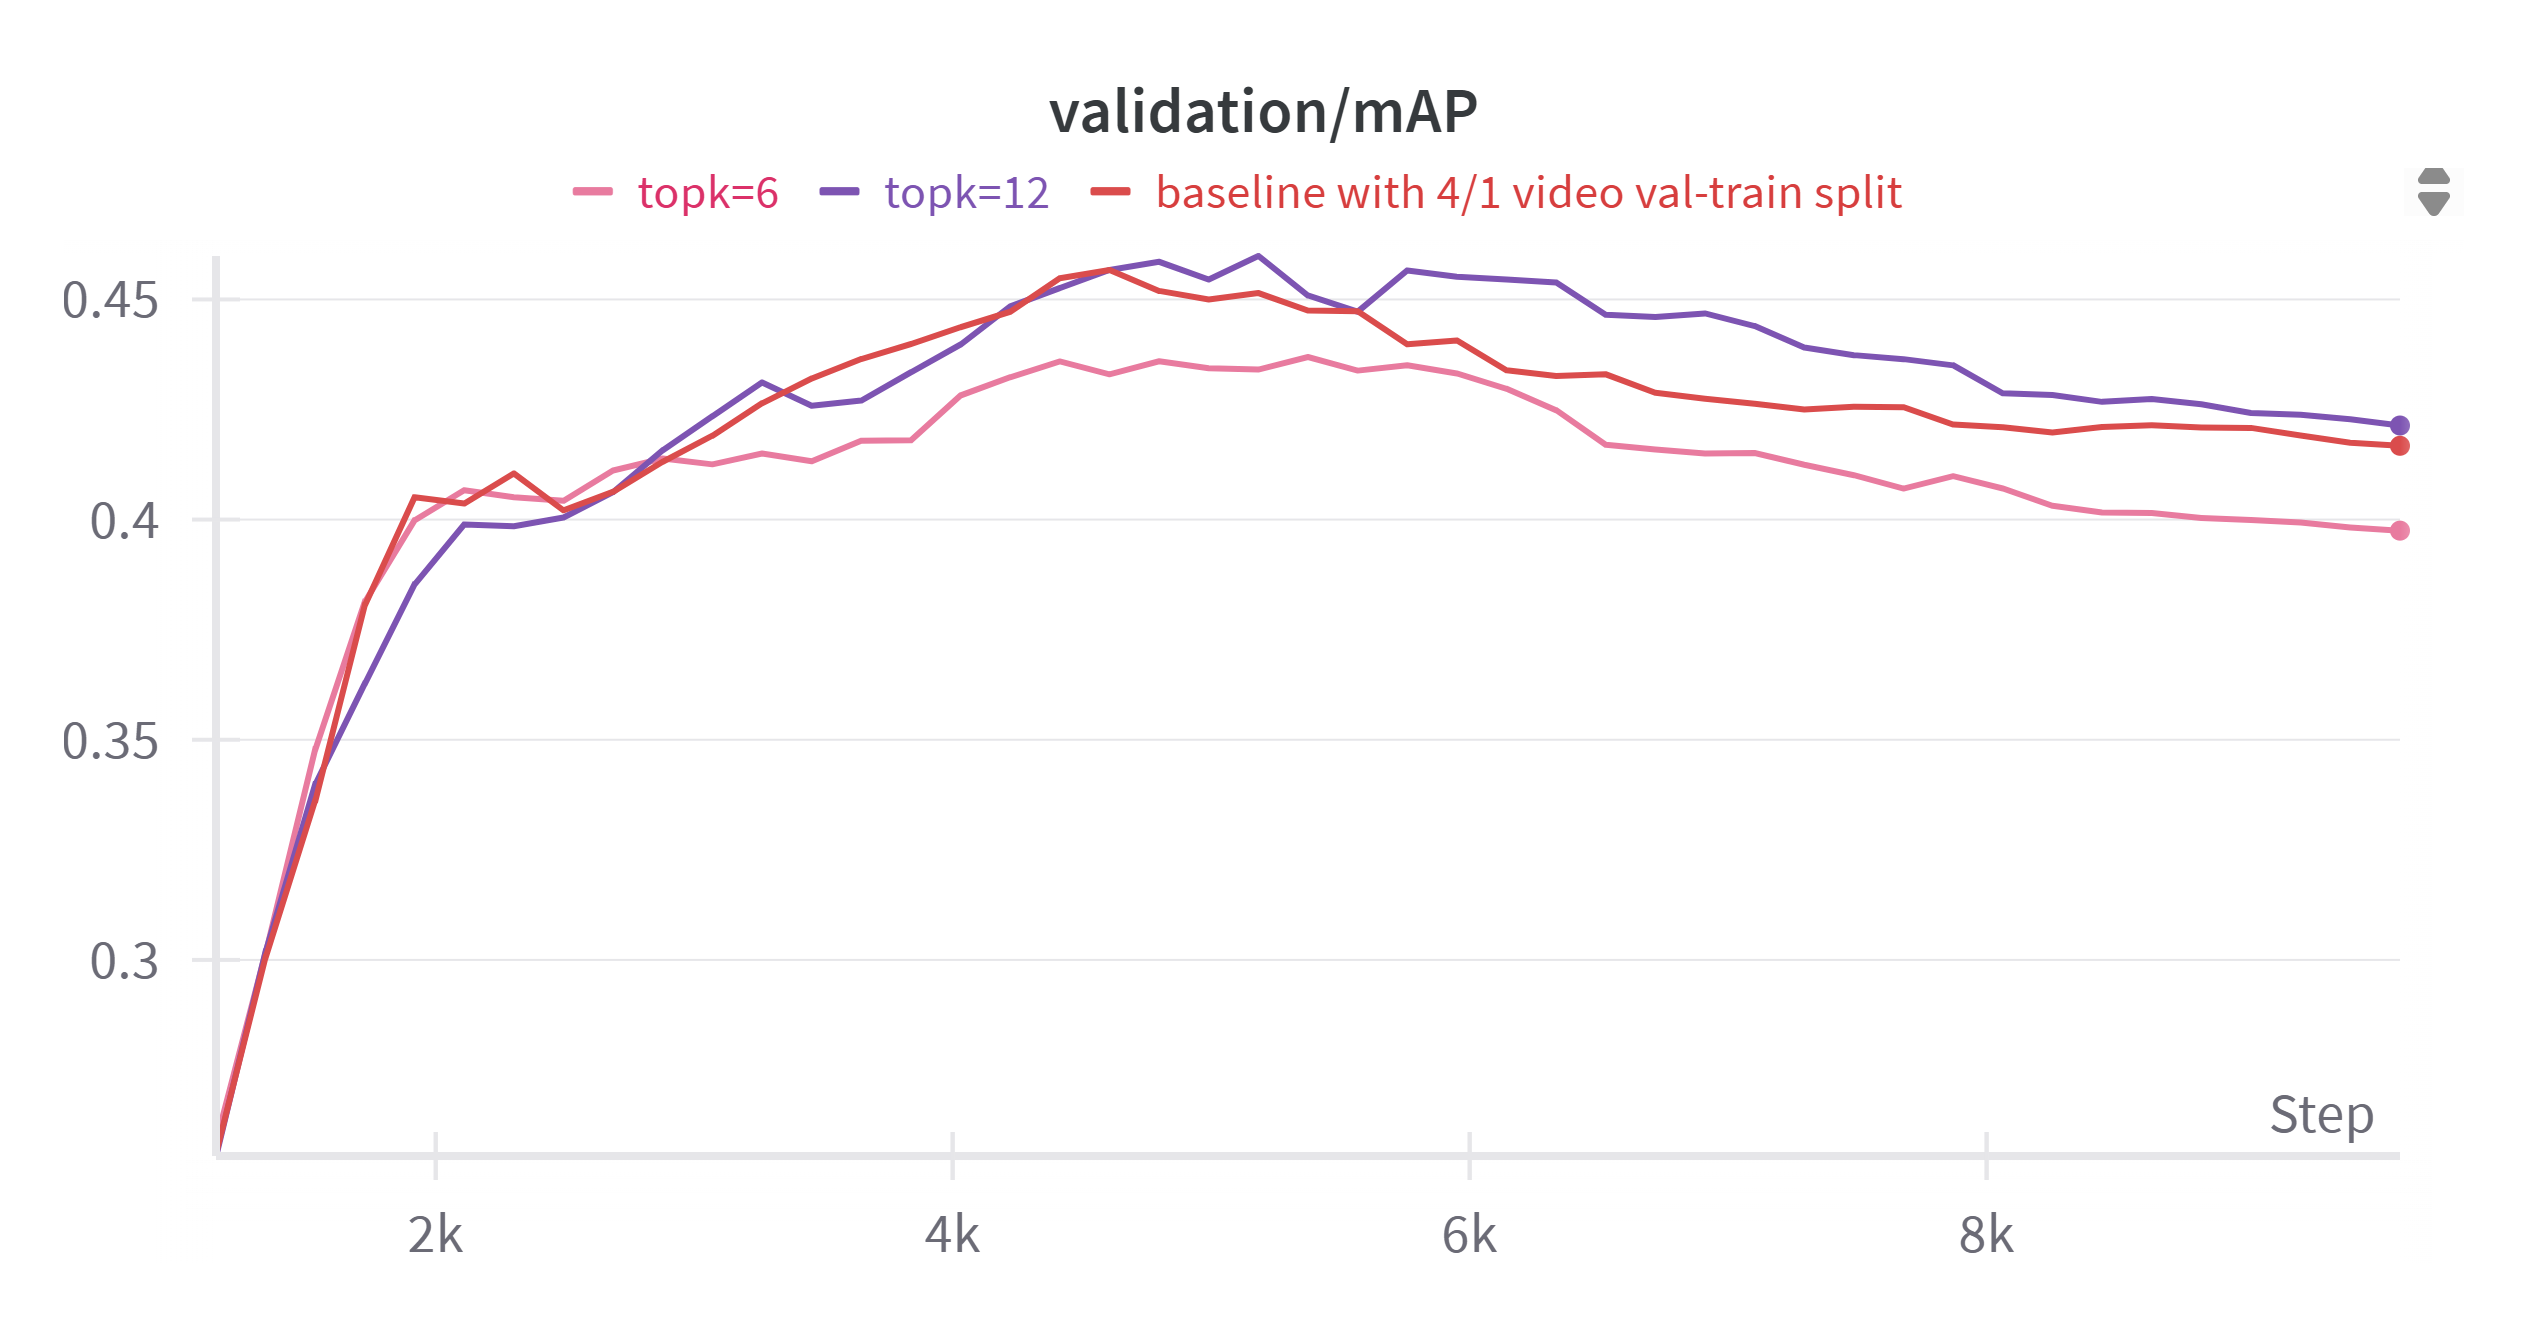
\includegraphics[width=0.75\linewidth]{figures/topk_classes.png}
    \caption{Results from different postprocessing top \(k\) classes.}
    \label{fig:topk}
\end{figure}

Using a shorter stride for validation is a technique to increase training speed. In the case of the \acrshort{tdeed} implemented for SoccerNet, the testing phase is weighted more heavily than validation, as it is the submission to a challenge. This is an oversight; a run with \(STRIDE=1\) was run but not completed in time for discussion. This oversight could hinder the direct comparison between the validation scores. \improvement{this is addressed in experiment 6}


The temporal discriminability enhancer part of the \acrfull{tdeed} has specialized strategies and components designed to:
\begin{itemize}
    \item improve the distinction between similar actions
    \item improve token discrimination
    \item per frame predictions
\end{itemize}

Focusing on enhancing temporal distinctions is one key to success in tasks where slight variations in timing or appearance can result in different categories. 

In contrast, Mamba's design captures long-range contexts and provides a broader understanding of the video. It is also meant to learn quicker with linear complexity and require less data. It is my theory that with a stronger postprocessing pipeline, the \acrshort{map} advantage would be larger. 

The validation set size of a single football game can be problematic. Football games can vary significantly due to teams, play styles, event frequency, and referee threshold for giving fouls, to name a few. There is a risk of bias from the distribution of actions within the validation game. If the validation game is "easy" or "hard," that would severely influence the score. A split of 80\% to 20\% validates on one game and trains on four in total. However, the validation set is more robust when the game is split into 90 sections randomly assigned to each category. The result will be more transferable and generalizable. The model with joint training in \cref{fig:500_7_val_compare}, varies a lot in its validation. I assume this is because of the inherited differences in validation clips. 

\acrshort{vms} runs on any \acrshort{gpu}, but \acrshort{tdeed} needs a lot of memory and only runs on premium GPUs. If computational resources (especially GPU memory and type) are a limiting factor, \acrshort{vms} is the more practical choice. \acrshort{vms} has simpler postprocessing and a clearer GitHub explaining installation steps, which could be more straightforward to deploy. However, without obvious comparisons, it is hard to pick out clear advantages of one model over the other. 

The most significant limitation is the absence of the test \acrshort{map}@50 score for the \acrshort{vms} model. This prevents a direct and complete comparison with \acrshort{tdeed} on this crucial metric, which is often considered the primary performance indicator on unseen test data.

The \acrshort{tdeed} model was evaluated differently for validation and testing. The validation used a stride of two (halving temporal resolution) and lacked significant postprocessing (like \acrshort{snms}). The test evaluation used a smaller stride and included such postprocessing. This inconsistency makes it difficult to:

\begin{itemize}
    \item Directly compare \acrshort{tdeed}'s validation \acrshort{map}@50 with its test \acrshort{map}@50.
    \item Fairly compare \acrshort{tdeed}'s validation \acrshort{map}@50 with \acrshort{vms}'s validation \acrshort{map}@50, as the evaluation conditions were not equivalent.
\end{itemize}

While \acrshort{tdeed}'s "four matches for training and one for validation" is an 80\%/20\% split, validating on a single match can be less representative and more prone to bias than an 80\%/20\% split.

Using default hyperparameters from their original papers" might not be optimal for the specific SoccerNet-V2 dataset or the fine-grained action spotting task. These defaults might have been tuned for different datasets or tasks, potentially disadvantaging one or both models. This is tackled in \autoref{sec:experiment4}.



\section{Experiment 2: Compare runtime}
\label{sec:experiment2}

Wall-clock training time for each model on a Tesla A100 \acrshort{gpu} was recorded. Feature extraction and inference time were timed. If no \acrshort{gpu} is mentioned, it is A100 which is applied. 

\subsection{Setup}
\label{ssec:ex2_setup}

The same runs used in \autoref{sec:experiment1} are measured. \acrlong{wandb}' metric for duration is measured. In addition, the preprocessing pipelines for each model are isolated and measured independently. A validation run is also done to measure the inference time of each model. A100 \acrshort{gpu}s are used, of size 80 GB or 40 GB, with an indifference to interpret the results. 

\subsection{Results}
\label{ssec:ex2_result}

\begin{table}[h]
    \centering
    \begin{tabular}{|c|c|c|}
        \hline
        Match & Time  & \acrshort{gpu}\\
        \hline
        Blackburn Rovers- Nottingham Forest & 5h 51min & Tesla V100-PCIE-32GB \\
        \hline
        Brentford - Bristol City & 5h 42min & Tesla V100-PCIE-32GB \\
        \hline
        Hull City - Sheffield Wednesday & 5h 42min & Tesla V100-PCIE-32GB \\
        \hline
        Leeds United - West Bromwich & 5h 54min & Tesla V100-PCIE-32GB\\
        \hline
        Middlesbrough - Preston North End & 5h 58min & Tesla V100-PCIE-32GB\\
        \hline
        Reading - Fulham & 5h 51min & Tesla V100-PCIE-32GB\\
        \hline
        Stoke City - Huddersfield Town & 10h49min & Tesla P100-PCIE-16GB\\
        \hline
        Wigan Athletic - Birmingham City & 5h32min & Tesla V100-PCIE-32GB \\
        \hline
        Cardiff City - Queens Park Rangers & 5h 45min & Tesla V100-PCIE-32GB \\
        \hline
        \hline
        \textbf{Average}(excluding Stoke v Huddersfield)= & \textbf{5h 47 min} & \textemdash \\
        \hline
    \end{tabular}
    \caption{The preprocessing times for all games. They are preprocessed using the \acrshort{vmae} pipeline. The average excludes the game between Stoke City and Huddersfield Town because it seems to have been a measuring error making it take twice as long. }
    \label{tab:average_feature_extraction}
\end{table}

\unsure{How important would it be to use A100s in this experiment. For: Comparability. Against: Show that vms runs on any gpu opposed to tdeed}



\begin{table}[ht]
    \centering
    \begin{tabular}{lccc}
        \toprule 
        Model & Preprocessing (1 game)  & Training(4+1 games) & Inference (1 game) \\
        \midrule
        \acrshort{tdeed} & 13 & 3267 & 5\\
        \acrshort{vms} (Mamba-\acrshort{s6}) & 342 & 43 & 0.1$(7s)$ \\
        \bottomrule
    \end{tabular}
    \caption{Time comparison. All times are measured in minutes. The inference time for \acrshort{vms} is also provided in seconds. The game between Blackburn Rovers and Nottingham Forest, lasting 96 minutes, took 7.47 seconds with an average of 0.08 seconds per minute-long clip. Inference time assumes the preprocessing is completed.}
    \label{tab:results_ex2}
\end{table}

\cref{tab:results_ex2} shows the time for each step in each model. The total training time for \acrshort{tdeed} is \(13min+3267min= 3280min\). To infer one game with \acrshort{tdeed} it takes \(13min+5min=18min\). Concurrently, \acrshort{vms} takes \(342min+43min=385min\) to train on five games. Inference time for one game is approximately the same time as the preprocessing of that game, in this case \(342min\). In both cases, full parallelizability is assumed in preprocessing and inference. 

\subsection{Discussion}
\label{ssec:ex2_discussion}
\todo{run tdeed runs, rn it is haakon data}

MAMBA is exceptionally quick in running inference on the games, and the bottleneck is the feature processing. Suppose the inference is parallelized over each of the $\approx90$ videos, which is very possible, and the inference time of a game. The inference would be complete before you can blink \cite{bartoshuk_blinking_1977}. Quick. The \acrshort{vmae} preprocessing pipeline is the bottleneck. Efforts should be made to decrease this. 


The same is not true for \acrshort{tdeed}. The model is relatively balanced between preprocessing time and inference time. A complete pre-processing and inference of a game takes 18 minutes. Comparing the full pipeline time between the two, the inference time, which is supposed to be one of the advantages of \acrlong{s6}s, is lost because of the preprocessing. 



Therefore, the direct comparison of preprocessing times (13 min for \acrshort{tdeed} vs. 342 min for \acrshort{vms}) is affected by the hardware difference in \acrshort{gpu}s. The actual difference in preprocessing efficiency on identical hardware might be less pronounced than these numbers suggest. \acrshort{vms} preprocessing would still likely be considerably longer. 


Both runs were run with early stopping mechanisms. If one compares \cref{fig:500_7_val_compare} and \cref{fig:plateu_sweep}, it is evident that both models converge before they end. A more aggressive early stopping would favor the \acrshort{tdeed} model. The difference in training time is still very significant. The training time of \acrshort{tdeed} also decreases the efficiency of a hyperparameter sweep. If each run takes two days, the effort expended to tune the \acrshort{tdeed} parameters is big. 


While A100 \acrshort{gpu}s of both 40GB and 80GB capacities were utilized, the specific workloads were generally not memory-capacity bound, and any minor runtime variations are not expected to alter the primary conclusions regarding relative model and preprocessing speeds. However, this constitutes a minor uncontrolled variable in the experimental setup. 


The assumption of full parallelization simplifies the comparison by looking at the theoretical maximum throughput. Practical implementations might face limitations that increase the observed times. Parallelization on feature extraction was done by queueing jobs on different \acrshort{gpu}s. Achieving perfect or full parallelization in real-world systems is challenging due to:
\begin{itemize}
    \item \textbf{Overhead}: Costs associated with managing parallel tasks (e.g., data distribution, synchronization).
    \item \textbf{Bottlenecks}: Parts of the pipeline that cannot be parallelized (e.g., serial I/O operations, certain algorithmic steps).
    \item \textbf{Resource Limits}: Finite number of CPU cores, GPU cores, or memory bandwidth.
\end{itemize}


For research involving frequent retraining or inference on already processed data, \acrshort{vms}'s model speed is a significant advantage. For deploying a model to process new, unseen games quickly from raw video to final output, \acrshort{tdeed}'s faster preprocessing currently gives it an edge in total time, despite its slower model component. The comparison is also impacted by:

\begin{itemize}
    \item The missing test \acrshort{map}@50 for \acrshort{vms}.
    \item The different GPUs used for measuring \acrshort{vms} preprocessing (V100s) versus \acrshort{tdeed} components (A100s).
    \item The inconsistencies in \acrshort{tdeed}'s validation and test procedures noted in Experiment 1
\end{itemize}


While a P100 \acrshort{gpu} is expected to be slower, the processing time of the Stoke City game was anomalously long. It was excluded from the average sum to provide a more representative preprocessing time for \acrshort{vmae}. The fact that it is $\approx2x$ times the time of the other runs suggests other issues. \improvement{test games with a100 to}

\section{Experiment 3: Feature increase}
\label{sec:experiment3}
To determine how much the size of the feature vector matters, a model with 1408 features and one with 3200 features were trained on the THUMOS-14 dataset.
InternVideo features have a size of 3200 and are the backbone of the \acrshort{sota} models on paperswithcode. The \acrshort{vms} models trained on Soccernet use 1408 features. Both models are trained with a Tesla V100-PCIE-32GB.


\subsection{Setup}
\label{ssec:ex3_setup}

To assess the effect of embedding size, two \acrshort{vms} instances were trained on THUMOS-14\cite{dataset:thumos}: one using 1,408-dimensional VideoMAE features and one using 3,200-dimensional InternVideo embeddings. All other settings, annotations, and hyperparameters remained identical.

The metrics are tracked using \acrlong{wandb} and console logs.
Both models were trained for 49 epochs on a Tesla V100-PCIE-32GB \acrshort{gpu}.

\subsection{Results}
\label{ssec:ex3_results}

\begin{figure}
    \centering
    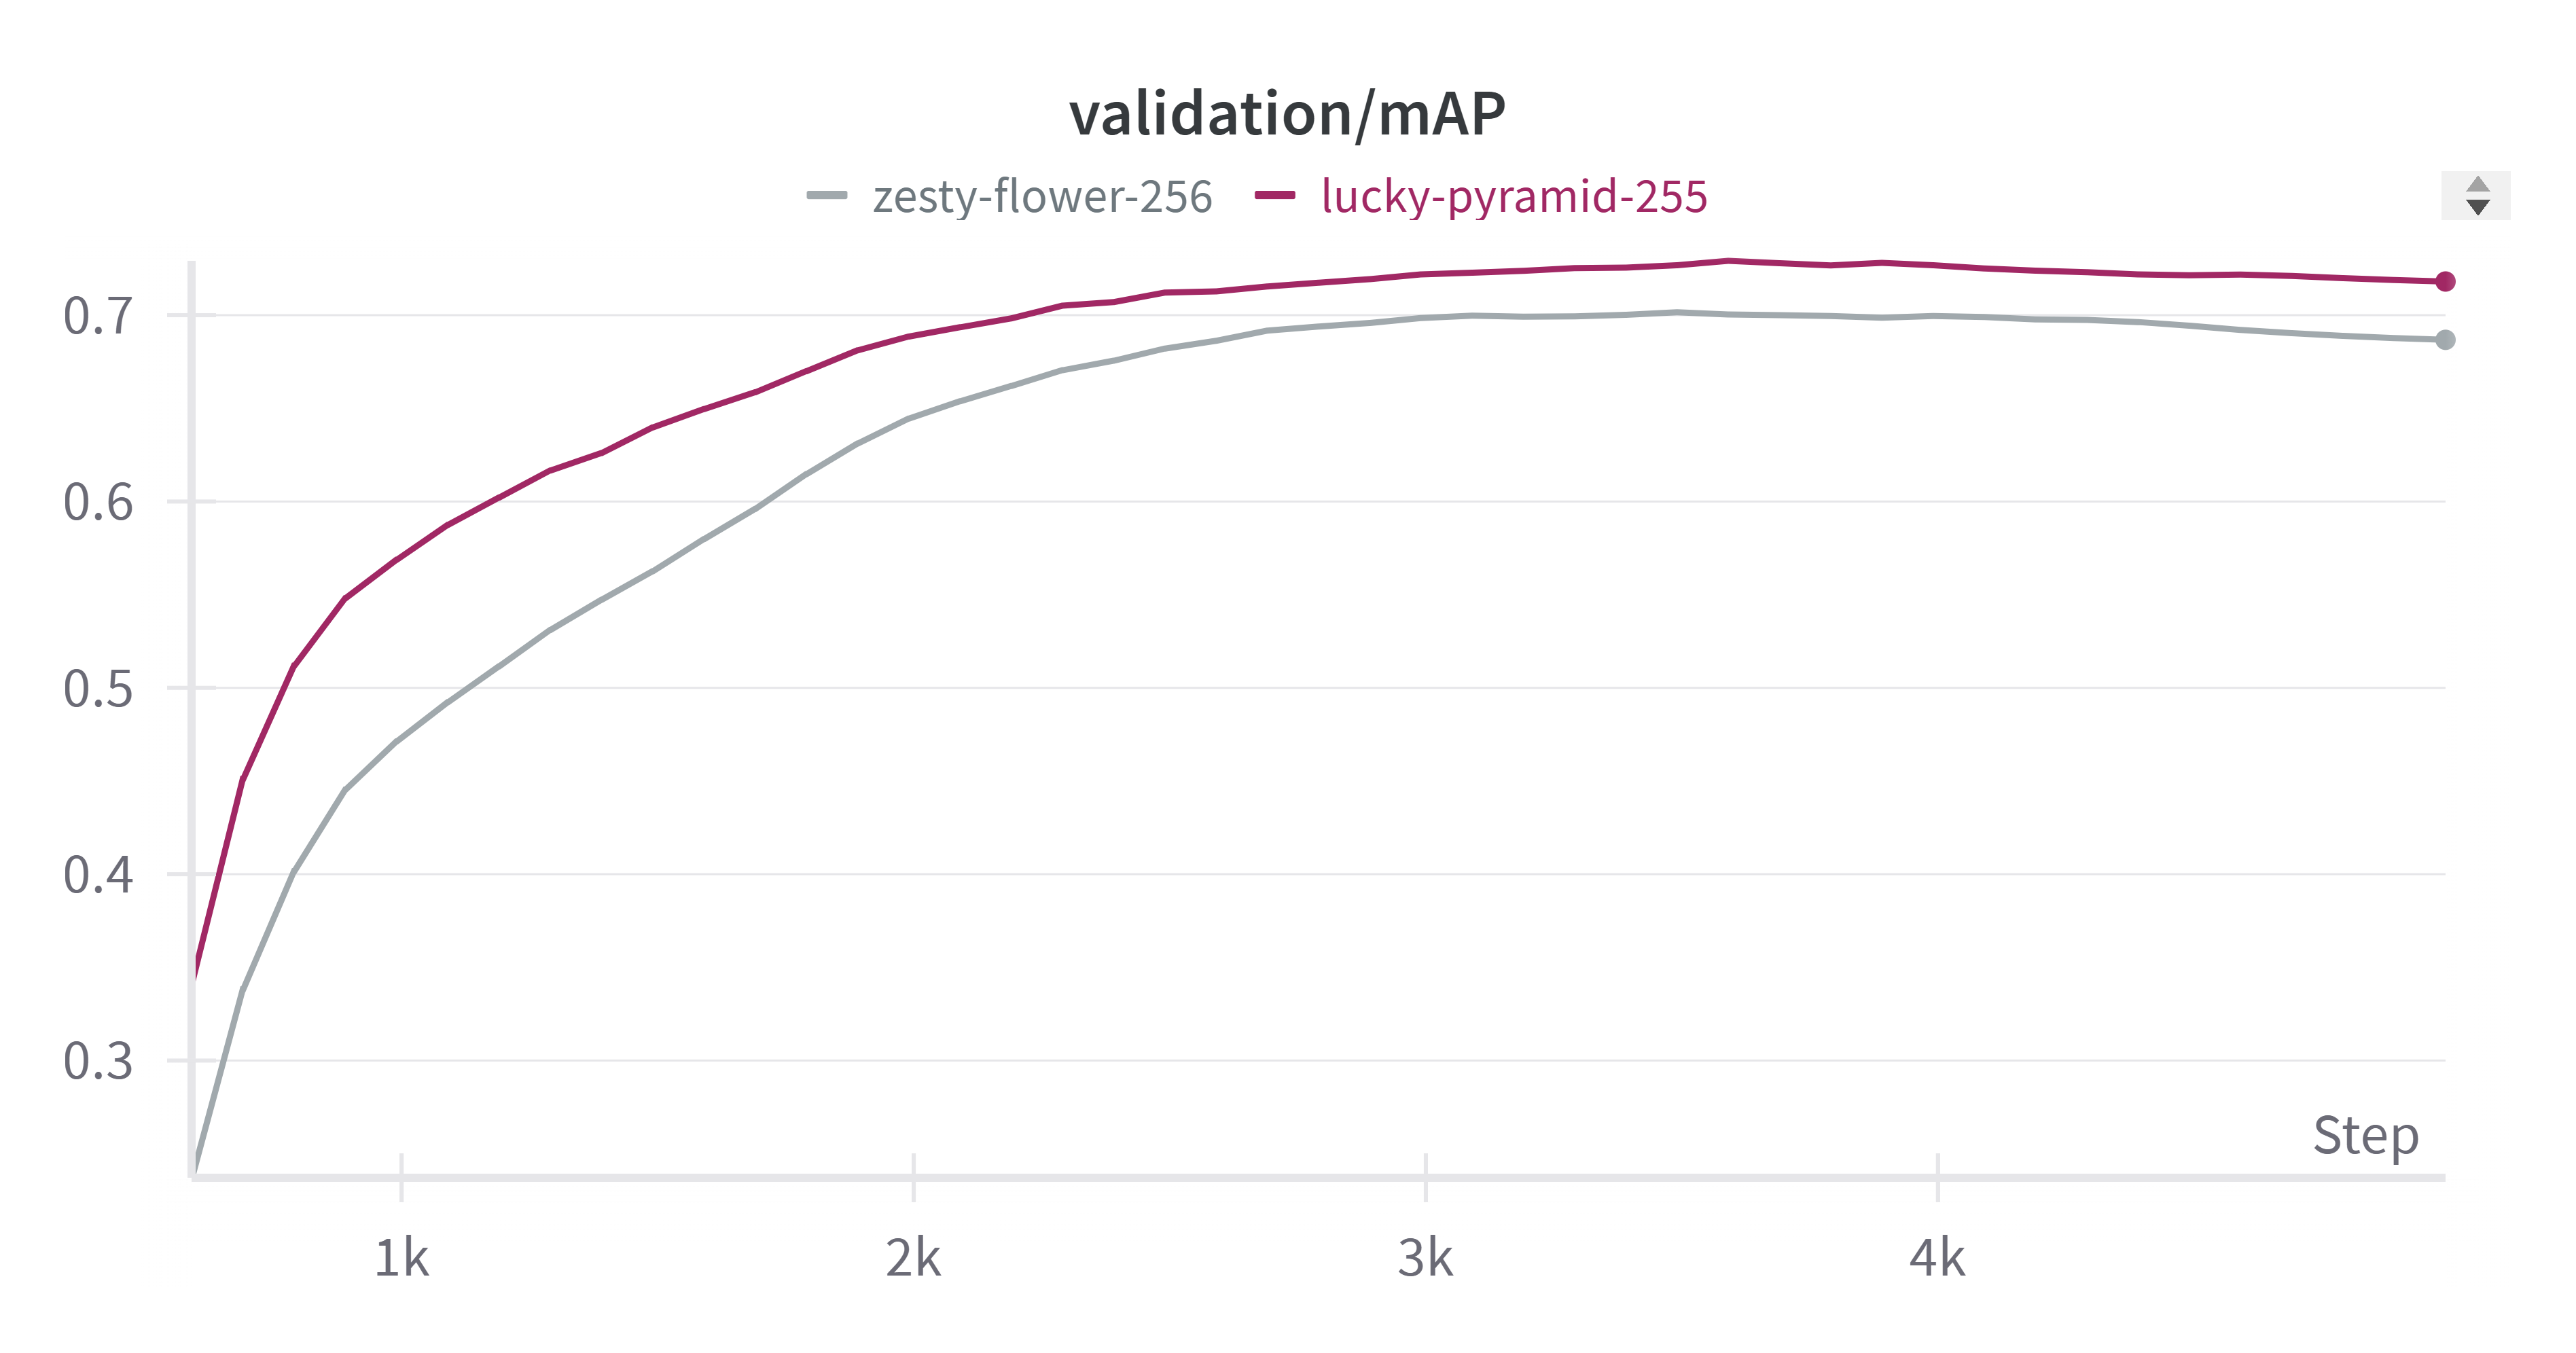
\includegraphics[width=0.75\linewidth]{figures/1408_3200_val.png}
    \caption{Validation per epoch for 3200 features (red) and 1408 features(grey). }
    \label{fig:ex3_val}
\end{figure}
The 1,408-dimensional model achieved a  \acrshort{map} of \(0.686\), while the 3,200-dimensional model reached a \acrshort{map} of \(0.718\) (a 3.2\% absolute gain). Training times were one hour and 15 min and 1 hour 23 min respectively, an increase of \(\approx11\%\). In \autoref{fig:ex3_val}, you can see how the model with more features outperformed the lower feature model from the first epoch to the last. 


\subsection{Discussion}
\label{ssec:ex3_discussion}


I am confident the $3.2\%$ increase stated in the results is a consistent improvement. As seen in \autoref{fig:ex3_val}, the improvement is consistent over all epochs. The slight drop in the 1408 feature validation score towards the end proves there might be some overfitting in that model, which is not evident in the other model. 


More dimensions inherently increase the probability of linear separability and provide greater capacity for the model to represent complex relationships. 3200 features, as opposed to 1408 features, are more likely to be separable by a simpler model. The increase in features increases the \textit{capacity} for better separation. 


InternVideo features are used in \acrshort{sota} models. This suggests they are pre-trained in a way that captures very rich and discriminative information relevant to video understanding tasks like action recognition. The 3200 dimensions of InternVideo likely encode more fine-grained details, temporal dynamics, or contextual cues than the 1408 dimensions of VideoMAE features. It is not just about having more numbers; these additional numbers represent meaningful variations beneficial for distinguishing actions in THUMOS-14.



In academic research or competitive benchmarking, a $3.2\%$ gain is significant. In the same environments, training times are a secondary concern. As a one-time training, both variants clock in at below 1h30min using a V100 \acrshort{gpu}; this is insignificant in the context of video training. \info{will write in experiment 2}. The tradeoff between training time and increased accuracy is favorable. 


\begin{figure}
  \begin{subfigure}{0.42\textwidth}
    \includegraphics[width=\linewidth]{figures/xabi_nigel.png}
        \caption{A foul play, retrieved from Bleacher Report\cite{wyman_2018}.} 
        \label{fig:serious_foul}
  \end{subfigure}%
  \hspace*{\fill}   % maximize separation between the subfigures
  \begin{subfigure}{0.42\textwidth}
    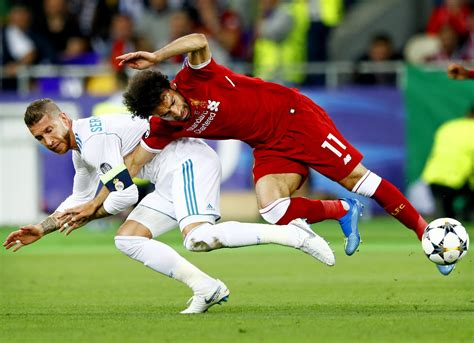
\includegraphics[width=\linewidth]{figures/salah_foul.png}
    \caption{A foul that looks different. Retrieved from The Athletic\cite{corrigan_2021}.} 
    \label{fig:another_foul}
  \end{subfigure}%
  \hspace*{\fill}   
  \caption{Two fouls highlight how unlike 'the same' action can appear. }
  \label{fig:different_fouls}
\end{figure}

Based on the findings from THUMOS-14, where higher dimensionality (3200 features) yielded a 3.2\% absolute \acrshort{map} gain over 1408 features, my hypothesis for football videos is that higher dimensionality would likely be beneficial and potentially even more critical. Football events have significant nuance, as shown in \autoref{fig:different_fouls}. At the same time, actions can be homogeneous. \acrshort{cv} does not understand depth in the same way as humans. One of the SoocerNet challenges this year is Monocular Depth Estimation. Understanding whether the ball is in the air(high pass) or on the ground (pass) is difficult. A higher dimensionality can find more hyperplanes to separate these actions on. 

I would hypothesize that the additional descriptive power offered by higher-dimensional features (like the 3200-dimensional InternVideo features) would be advantageous for capturing the subtle discriminative information needed to accurately spot and classify nuanced events in football videos, potentially leading to a similar or even greater performance improvement than observed in THUMOS-14.






The default hyperparameters are fit to 3200-dimensional features. This might boost its accuracy compared to a default set for 1408-dimensional features. However, as will be discussed in Experiment 3 in \autoref{sec:experiment3}, hyperparameters are deemed to have little impact. They are trained on 1408 and struggle to improve over the results from the default parameters. The \acrshort{map} gain could be smaller if hyperparameters were tuned for 1408, but there are no signs that it would be a significant difference from my experiments. 



The 3.2\% absolute \acrshort{map} gain with 3200-dimensional features over 1408-dimensional features suggests that opting for higher-dimensional, more expressive features can lead to significant performance improvements in action spotting. The \(\approx11\%\) increase in training time for the observed accuracy gain is a tradeoff to consider. For applications where accuracy is paramount and the additional training time is acceptable (especially given it was only 8 minutes longer in this specific experiment), using richer features is advisable.


\section{Experiment 4: Hyperparameter optimization}
\label{sec:experiment4}

The fourth experiment is a hyperparameter optimization experiment.
The goal is to find the best hyperparameters for the \acrshort{vms} model on the SoccerNet dataset.

\subsection{Setup}
\label{ssec:ex4_setup}

\acrlong{wandb} is used to track the hyperparameters and the results for the \acrshort{vms} model trained on the SoccerNet-V2 dataset with a 70 \(\%\)-30\(\%\) validation split. All seven videos of the SoccerNet V2 format are considered in this approach, including the training, validation, and testing videos. A Bayesian optimization algorithm is used to find the best importance and correlation of the hyperparameters. The hyperparameters related to the dataset are the only ones modified. Full details about the hyperparameters can be found in \autoref{app:sweep}.

A total of 210 runs across three sweeps of 70 runs each were completed. Because of the fast convergence of \acrshort{vms}--models hyperparameter search was an efficient process. 


\subsection{Results}
\label{ssec:ex4_results}

\begin{figure}[ht]
    \centering
    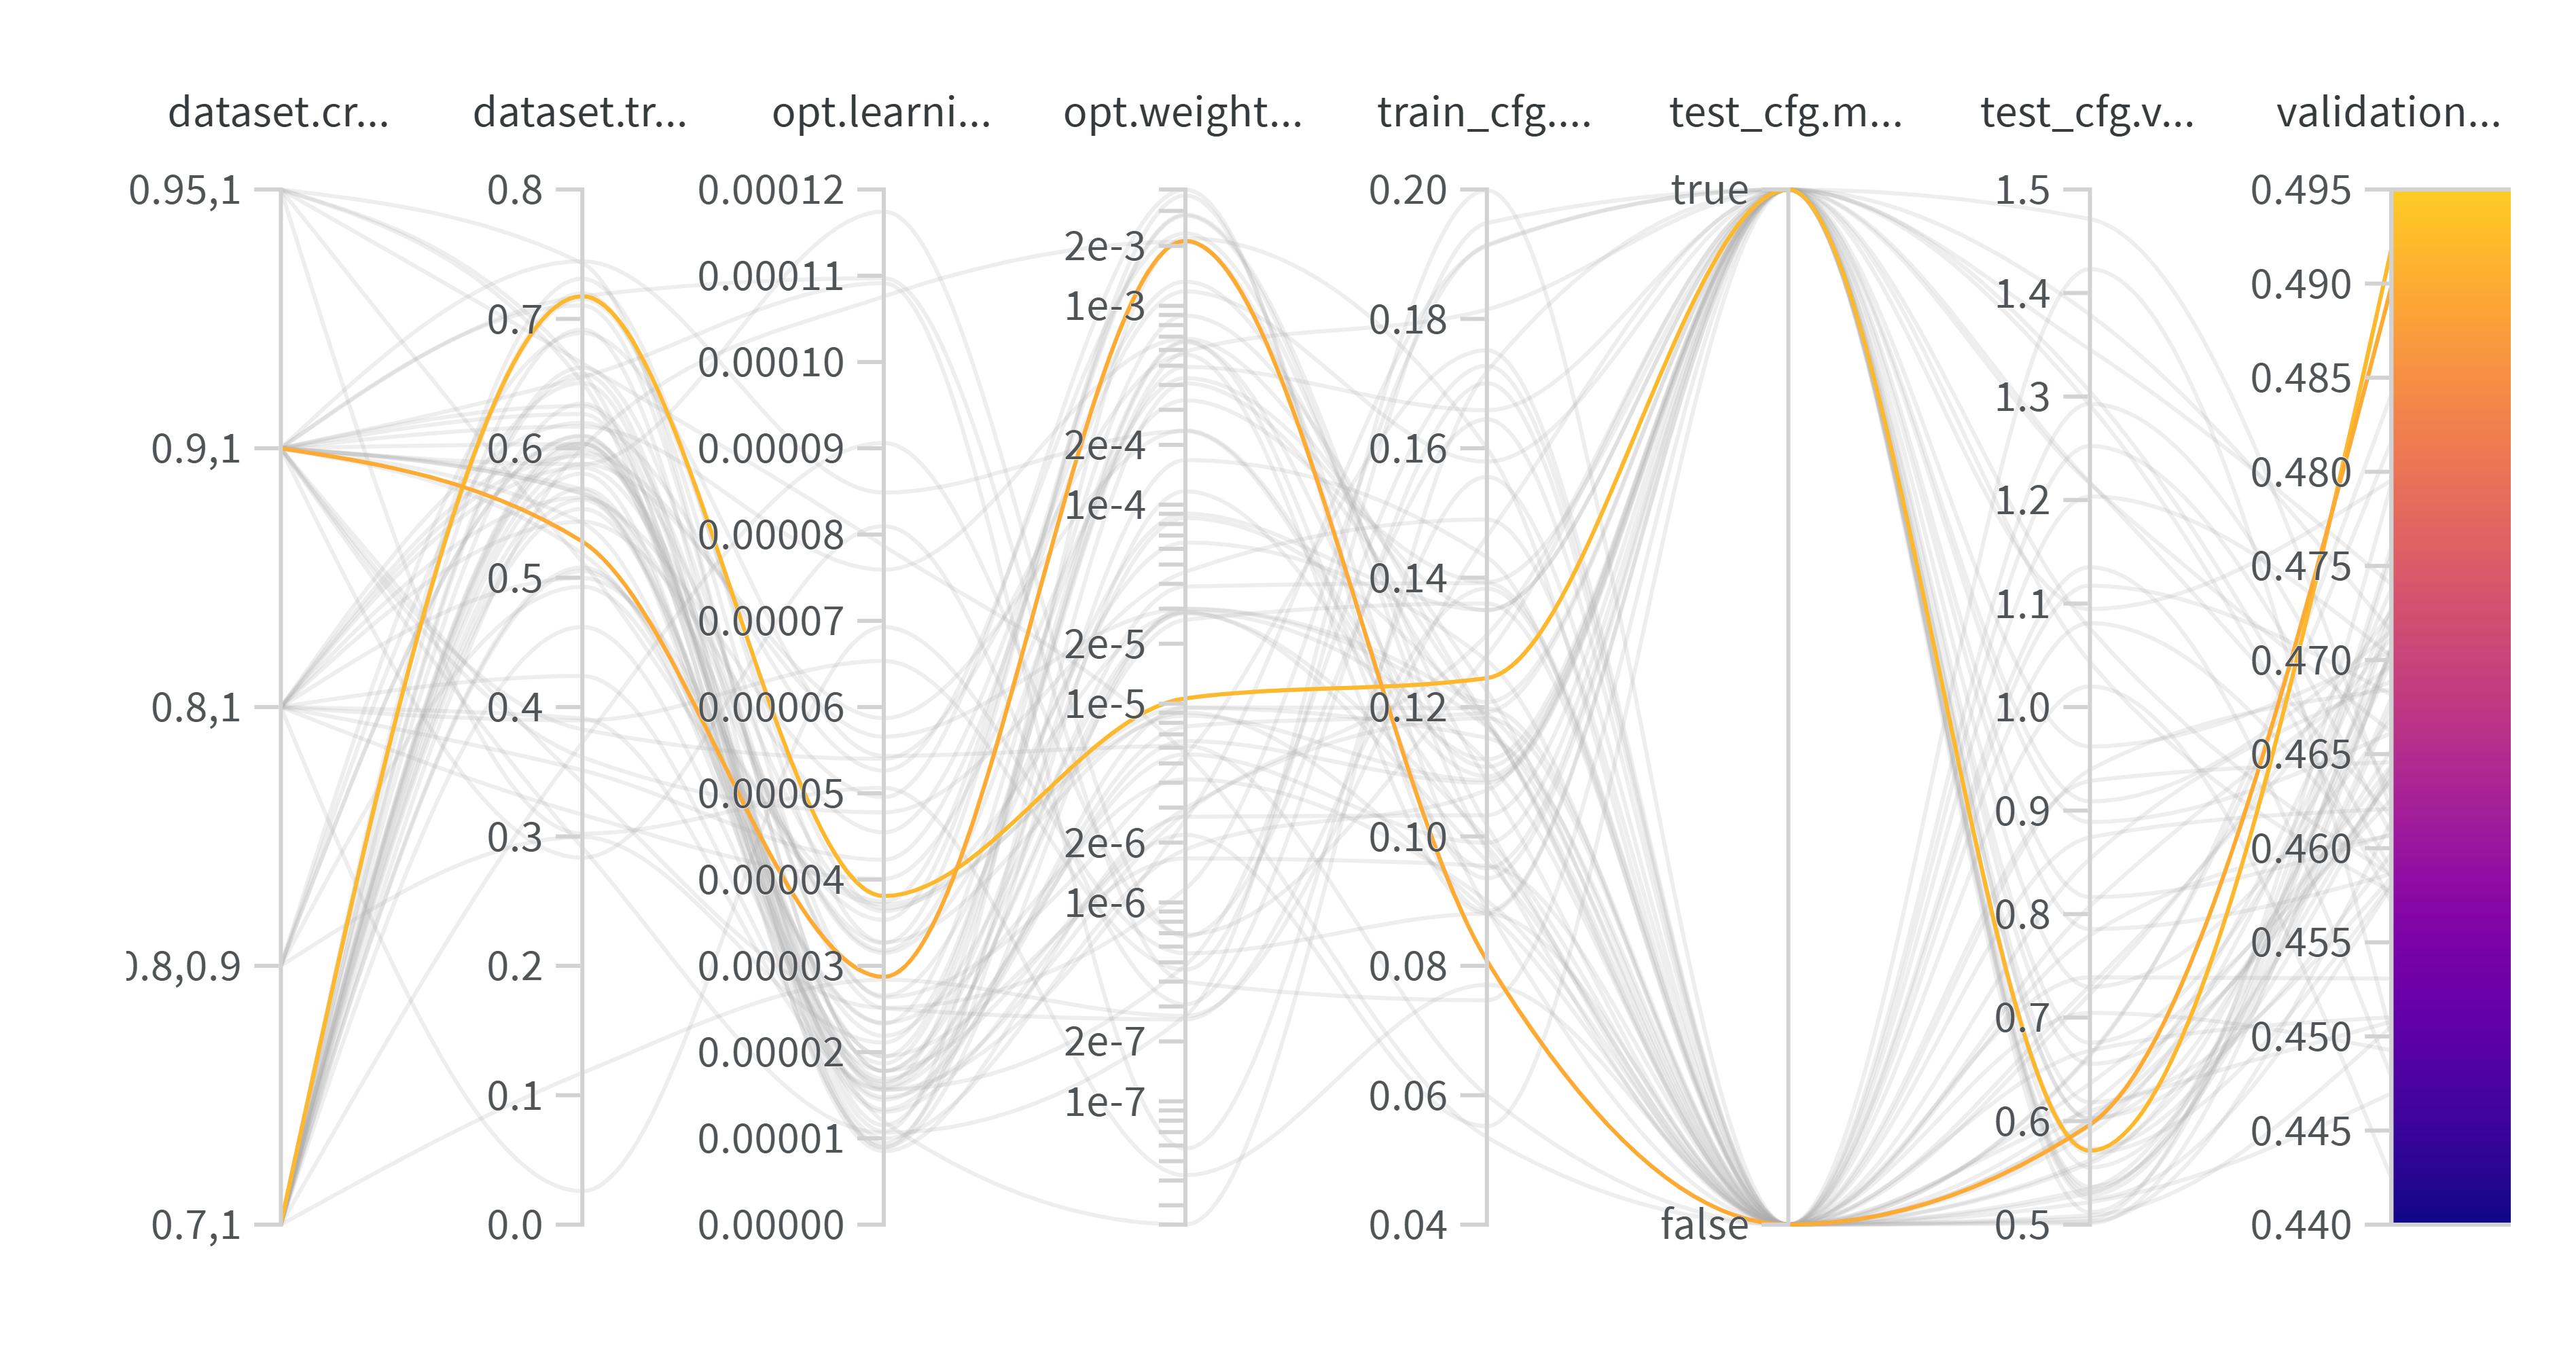
\includegraphics[width=1\linewidth]{figures/sweep_two_best.png}
    \caption{The hyperparameters of the two best results(yellow) compared to all runs (grey) in the third sweep. }
    \label{fig:sweep_best_two}
\end{figure}

The sweeps showed a slight improvement in the model. 

Trying to translate the sweep into a single better configuration did not prove helpful, but some configurations performed exceptionally better than the rest. However, these configurations that worked well had quite different parameters and were hard to differentiate. As seen in \autoref{fig:sweep_best_two}, the hyperparameters of the best and second-best run in the last sweep differed significantly in their hyperparameters. 

Interpreting the results to create a hyperparameter configuration, as explained in the \autoref{app:sweep_3}, the resulting average \acrshort{map} was \(46.77\%\). 

\subsection{Discussion}
\label{ssec:ex4_discussion}


\begin{figure}
    \centering
    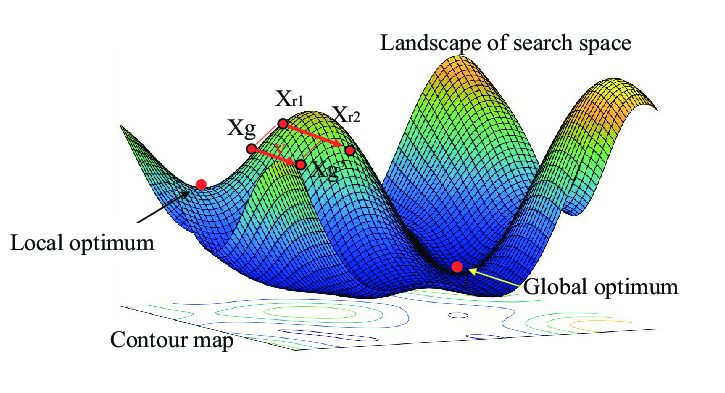
\includegraphics[width=0.75\linewidth]{figures/local_minima.png}
    \caption{A plot of local minima from \cite{fig:multiple_local_minima}. It is not related to any experiments done, but its purpose is as a visualization.}
    \label{fig:local_minima}
\end{figure}

It was not easy to translate the sweep into a single, consistently better configuration despite some exceptional outliers. This likely stems from a few different factors. \unsure{multiple local minima, describe in the background? Bad figure?}

The hyperparameter space might contain multiple local optima. This means there is not a "peak of performance," but several combinations of hyperparameters cause good results. Picking an average and combining parameters from distinct optima can result in a configuration. For the sake of visualization, look at \autoref{fig:local_minima} and imagine the summits are optima. Picking an average between them will perform worse than individual peaks. 

Hyperparameters often interact in complex and non-linear ways. The success of an \emph{exceptionally better} configuration might depend on a specific interplay between multiple parameters. Changing one parameter in an attempt to generalize or create a "single best" might disrupt this delicate balance, leading to suboptimal performance. The fact that the best two runs had "quite different parameters" (as seen in \autoref{fig:sweep_best_two} supports this idea of different, successful combinations rather than a single clear trend.


These two runs imply that multiple good configurations exist. The interaction between the parameters matters more than the individual values. A specific value for one hyperparameter might work well only in conjunction with others. The two good runs in \autoref{fig:sweep_best_two} could represent two good synergies. 


If the hyperparameter landscape had a dominant global optimum, one would expect the best-performing runs to converge towards similar hyperparameter values. The fact that two distinct sets of parameters yield top results suggests that there are at least two separate "peaks" or favorable regions (local optima) in the search space where the model performs exceptionally well. The optimization process has found these different peaks rather than a single point.

This implies some broader challenges for hyperparameter tuning:

\begin{itemize}
    \item Difficulty in Identifying a Single "Best" Configuration: It becomes hard to declare one set of hyperparameters universally optimal. What works best might be one of several good combinations.
    \item Increased Search Complexity: Optimization algorithms can easily get "stuck" in a local optimum, potentially missing a better global optimum or other strong local optima. This necessitates more sophisticated search strategies or more extensive random sampling to explore the space adequately.
    \item Sensitivity to Initial Conditions: The starting point of a hyperparameter search can heavily influence which local optimum is discovered.
    \item Challenges in Interpretation: It is harder to draw simple conclusions about the individual impact of each hyperparameter, as their optimal values might be highly dependent on the values of other interacting parameters, leading to different "optimal" combinations.
    \item Reproducibility and Generalization: A specific local optimum found might be particular to the exact dataset split or even the random seed used during the sweep. Generalizing these findings to slightly different conditions can be more challenging.
\end{itemize}



As seen in \autoref{app:sweep_3}, the best runs in the end show that the learning rate of the top-performing runs was relatively low. The Bayesian search preferred exploring lower learning rates, and especially the third sweep showed low learning rates performed best. In the last sweep, the learning rate had the highest importance and absolute correlation. The correlation was negative. 

A lower learning rate allows the model to make finer adjustments in homogeneous data like football actions, where events can be visually similar. This can help it learn the subtle distinguishing features without overshooting the optimal weight configurations in the loss landscape, leading to better discrimination between closely related actions.


The hyperparameters that were tuned are:
\begin{itemize}
    \item learning\_rate
    \item weight\_decay
    \item drop\_path 
    \item batch\_size (explored in Sweep 1, then fixed)
    \item voting\_thresh
    \item trunc\_thresh
    \item crop\_ratio (introduced in Sweep 3)
    \item multiclass\_nms (evaluated in Sweep 3)
    \item max\_seq\_len (explored initially, then ignored)
    \item pre\_nms\_topk (explored initially, then ignored)
    \item clip\_grad\_l2norm (explored initially, then ignored)
\end{itemize}

\textbf{Learning rate} appeared to be the most significant value. While its correlation varied, Sweep 3 indicated that the best performance was concentrated in a particularly low range (around 0.00003-0.00004). 

\textbf{Crop ratio} showed apparent performance differences between its settings. As the data augmentation parameter, it was expected to have a higher impact than it did. 

\textbf{droppath} was the most important with the least correlation in the first sweep. It was tuned in Sweep 2 and selected as a fixed value for Sweep 3. 

Sweep 1 deemed \textbf{batchsize} to be unimportant. Ideal values were found for voting\_thresh and trunc\_thresh in Sweep 3. 



The interpreted sweep configuration achieved an average \acrshort{map} of $46.77\%$. Default parameters on the same dataset got $48.73\%$ average \acrshort{map}. This is a significant decrease in performance of almost $2\%$. When comparing the same data split (70\%/30\% using all seven videos), the default hyperparameters outperformed the configuration derived from interpreting the sweep results. This suggests that creating a single "interpreted" set of hyperparameters was unsuccessful in finding a configuration superior to the defaults for this specific dataset setup.

The best run in the sweep got a $49.18\%$ average \acrshort{map}. That is $2.41\%$ higher than the interpretation and $0.45\%$ higher than the default parameters. It identifies that the sweep identified some configurations that outperformed the default, but an interpreted result did not exist. 



The features from \acrshort{vmae} are implicitly optimized to represent video information based on the original preprocessing pipeline. The ability to improve performance could be limited if the features are "happiest" when processed in a way that mirrors the feature extraction. It could be that the dataset hyperparameters are tuned to the feature structure, not the feature content, to some extent. The tuning might then explore variations that do not fundamentally alter or improve upon the information already captured by the features. 

Results indicate that while minor gains are possible through extensive tuning, the default \acrshort{vms} hyperparameters seem to be a very effective starting point for the SoccerNet dataset. The hyperparameter space explored, while yielding some improvements, did not reveal overwhelmingly superior configurations.


\begin{figure}
    \centering
    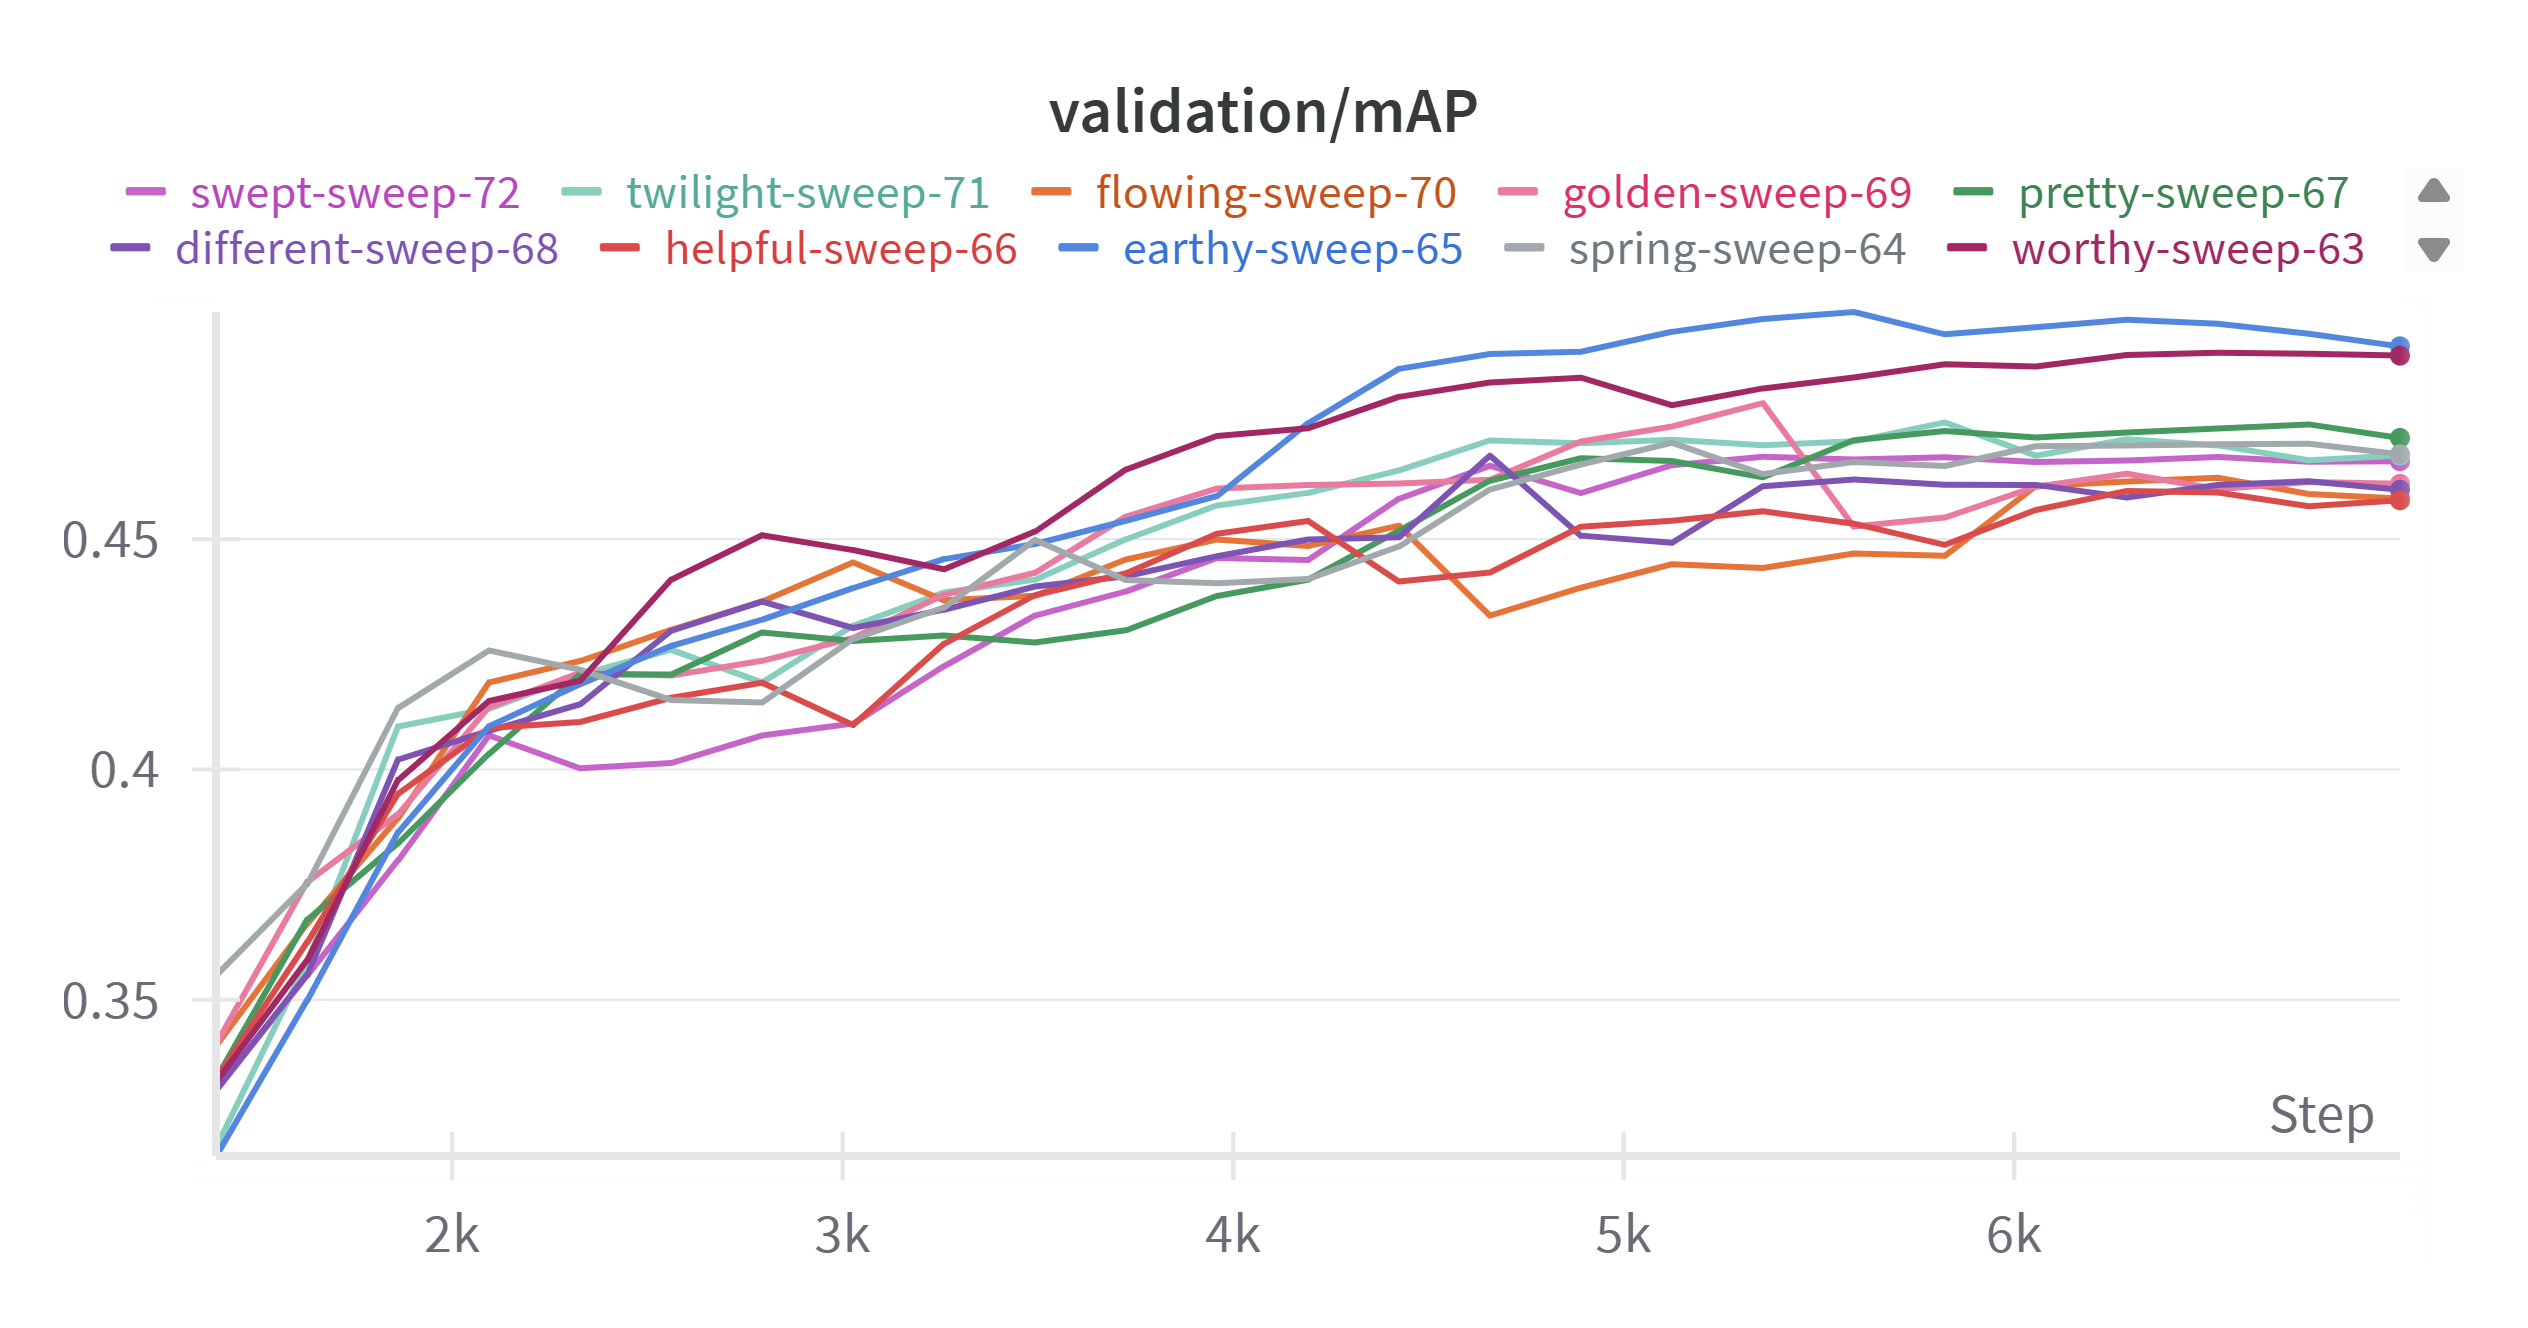
\includegraphics[width=0.75\linewidth]{figures/plateu_sweep.png}
    \caption{Validation plotted against steps for the latest runs in Sweep 3. }
    \label{fig:plateu_sweep}
\end{figure}
\begin{figure}
    \centering
    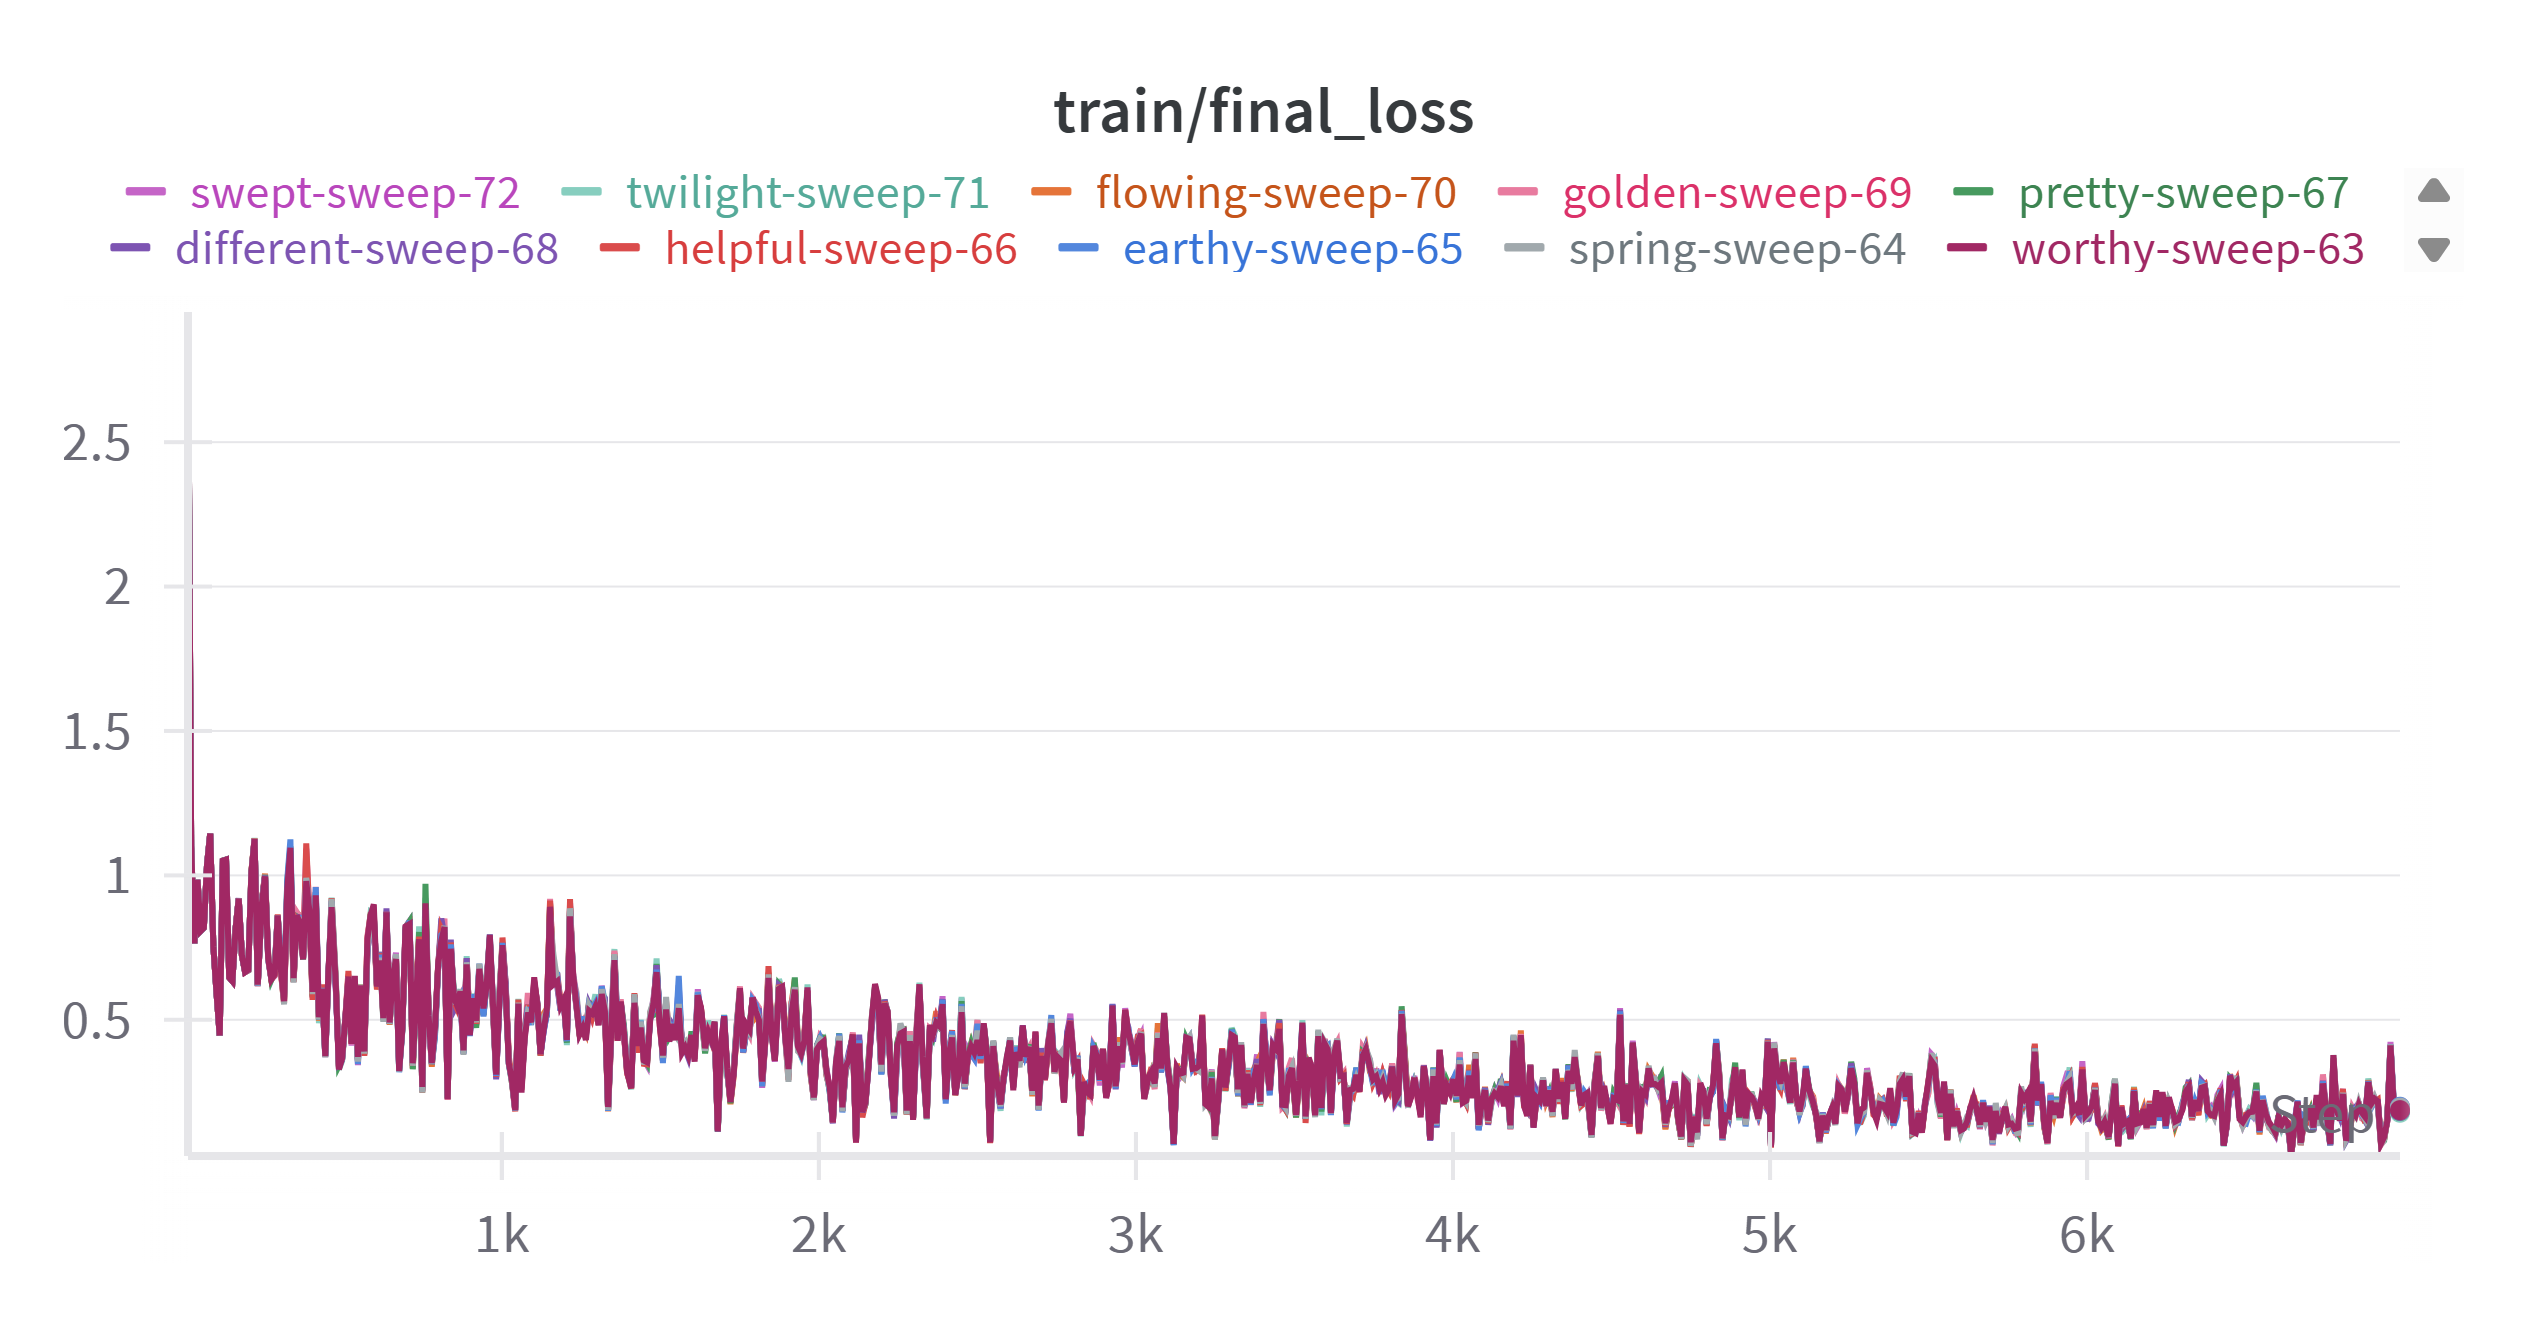
\includegraphics[width=0.75\linewidth]{figures/plateu_loss.png}
    \caption{Training loss plotted against steps for the latest runs in Sweep 3.}
    \label{fig:plateu_loss}
\end{figure}
The general trend of the sweep was for the runs to plateau relatively early, as seen in \autoref{fig:plateu_sweep}. At the same time, the loss was relatively low and stable. This indicates that the model stops generalizing to validation data and fits to noise in training data.


Bayesian optimization aims to find the best hyperparameters in fewer iterations. The algorithm is suited for a landscape with multiple optima because there is no inherent assumption of a single optimum. As seen in the Sweeps, some excellent runs were found compared to the average. 

Random search is effective for initial exploration. It has a use case if the initial parameters are considered close to a local optimum, which is not the global optimum. I had no reason to believe this, nor the motivation to explore enough variables compared to the original authors\cite{li_videomamba_2024}.


It might have been beneficial to start with a more extensive exploration before running the Bayesian search. This would require much more than the 210 runs on \acrshort{idun}, which was already under pressure. I find it probable that the default parameters, second \acrshort{sota} on the THUMOS benchmark, are close to the global optima. For sustainability, concerning power usage and fair usage of computational resources, I think it is correct not to continue the search. If the results showed a greater increase, the decision must be reconsidered.




This experiment increases my confidence in Experiment 1's results. It proves that the default hyperparameters perform well. The sweeps only slightly increased accuracy, and their interpretation performed worse. It demonstrates that the performance reported in Experiment 1 is a fair representation.

Experiment 1 mentioned that \textit{Using default hyperparameters from their original papers might not be optimal for the specific SoccerNet-V2 dataset - \cref{ssec:ex1_discussion}.}. Experiment 4 explored this for \acrshort{vms} and found its defaults were already firm. However, \acrshort{tdeed} was not subjected to a similar hyperparameter optimization. Therefore, while there is more confidence that \acrshort{vms}'s default performance is close to its tuned potential on this dataset, the same cannot be said for \acrshort{tdeed}. \acrshort{tdeed} might still have untapped potential if its hyperparameters were similarly optimized for SoccerNet.



To conclude:
\begin{itemize}
    \item \textbf{Default Hyperparameters are Robust}: The default hyperparameters for \acrshort{vms} provide a strong baseline. Extensive tuning might only yield marginal gains, suggesting that the original authors provided well-chosen defaults. This implies that for future comparisons or new experiments, starting with defaults is a reasonable approach, and significant deviations in performance are more likely due to other factors (model architecture, data, etc.) than suboptimal default settings.
    \item \textbf{Hyperparameter Optimization is Complex and Not Always a Silver Bullet}: The search space can have multiple local optima, making finding a single, universally "best" configuration difficult. Creating an "interpreted" best configuration from a sweep might not outperform the defaults or the best individual run found. This cautions against over-reliance on hyperparameter sweeps to unlock performance gains if a model is already well-designed.
    \item \textbf{Learning Rate is a Key Lever, Especially for Homogeneous Data}: For datasets like SoccerNet, where actions can be visually similar, a lower learning rate appears beneficial. This is a concrete takeaway for tuning \acrshort{vms} on such data.
    \item \textbf{Pre-trained Features Influence Tuning}: The characteristics of pre-trained input features can constrain the effectiveness of tuning downstream hyperparameters. The features might already be optimized for a specific processing "timeline," limiting how much dataset-specific tuning can improve things.
    \item \textbf{Resource Constraints and Practicality}: Exhaustive hyperparameter search is computationally expensive. The decision to stop searching must be balanced against the potential for gains and available resources, especially if initial results (like strong default performance) suggest diminishing returns.
    \item \textbf{Impact on Comparative Experiments}: The finding that \acrshort{vms} defaults are strong lends more credibility to comparisons made using these defaults (like in Experiment 1). However, it also highlights that the comparison might not reflect its potential if a competing model were not similarly tuned.
    \item \textbf{Focus on Broader Factors}: Given the modest gains from hyperparameter tuning, other factors like feature quality (Experiment 3), model architecture, data augmentation, and postprocessing strategies might offer more significant avenues for performance improvement.
\end{itemize}


\section{Experiment 5: \acrshort{tdeed} with and without joint training}
\label{sec:experiment_5}

The experiment compares two runs using the \acrfull{tdeed} model. The goal is to discover the performance loss by ignoring annotated games for a different action-spotting challenge. 

\subsection{Setup}
\label{ssec:ex5_setup}

\textcite{cioppa_soccernet_2024} provide the implementation of the \acrshort{tdeed} designed to train on all annotated games. The model is adapted to train on the \acrshort{snb} games, not the full dataset. \acrshort{map} per class, validation \acrshort{map}, test loss and compute time are the metrics used. 

The models are run with default hyperparameters and differ only in the dataset size. The difference in the dataset is that the grander datasets' classes are broader. \todo{mention in dataset section}. There are 12 classes from team events, like corners, goal kicks, etc. The newer dataset has annotations for whether the left or the right team is doing an action, while the older dataset does not. The default hyperparameters are designed for the old challenge. 


\subsection{Results}
\label{ssec:ex5_results}

\begin{figure}
    \centering
    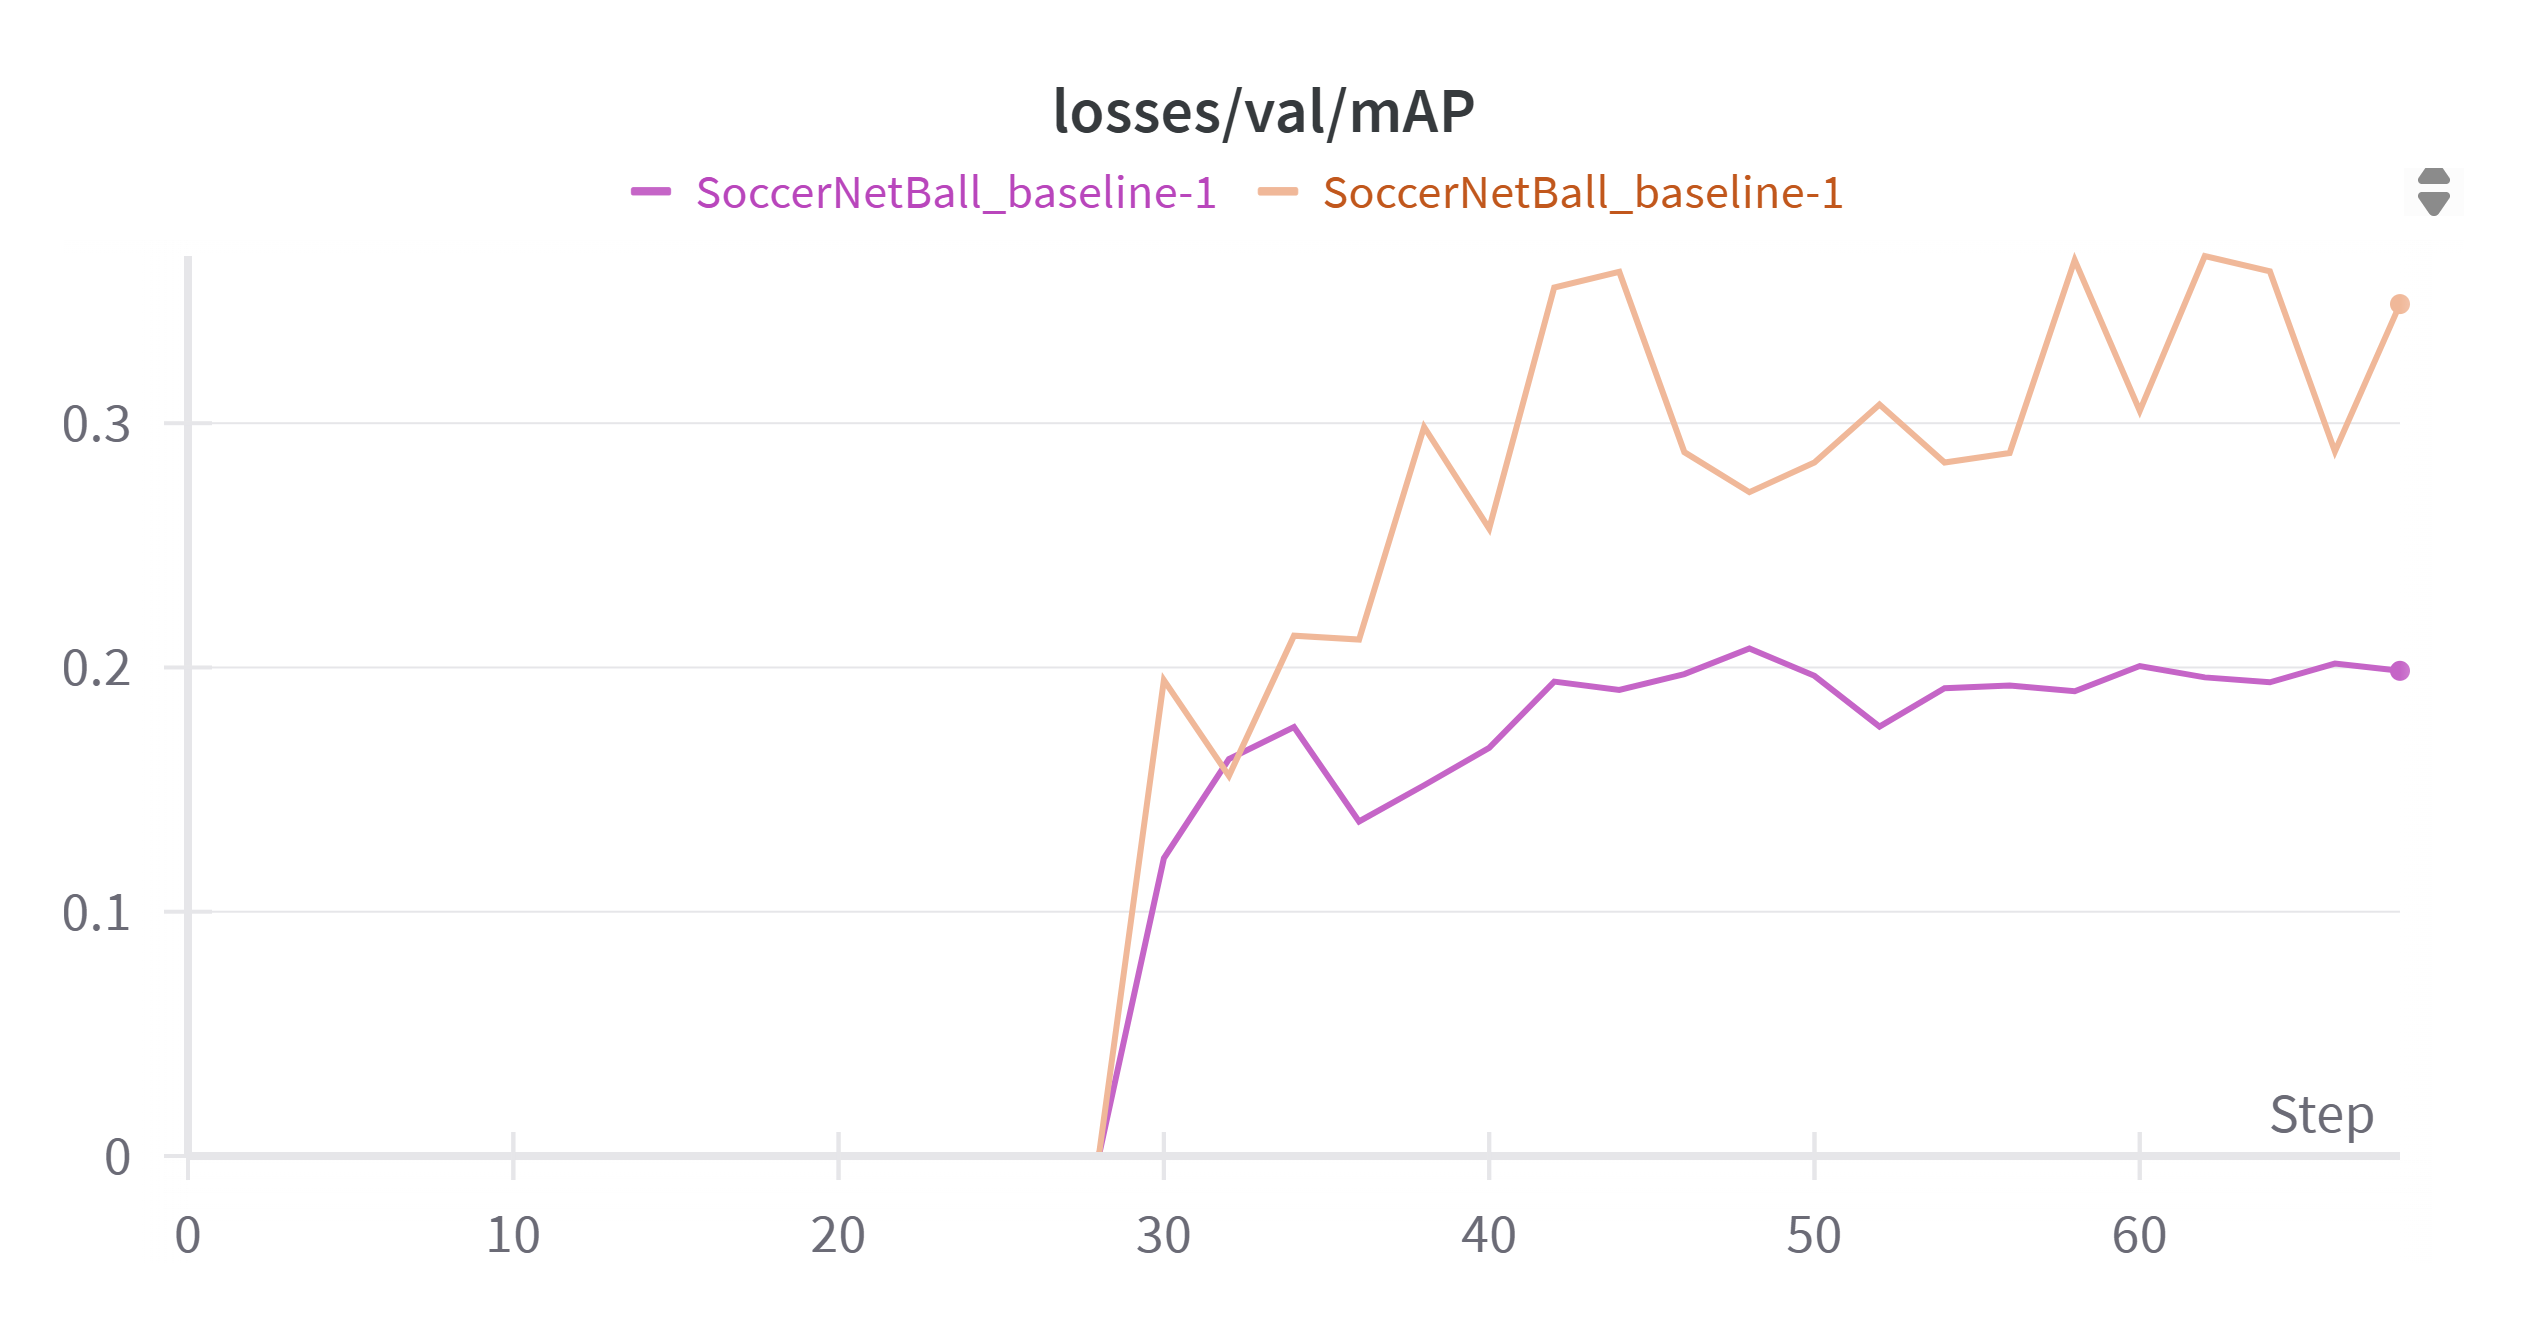
\includegraphics[width=0.75\linewidth]{figures/500_7_val_compare.png}
    \caption{Validation per epoch for the model trained with joint training (507 videos) (brown) and the model trained without joint training (purple). The models achieved a max \acrshort{map} of $36.84\%$ and $20.78\%$. }
    \label{fig:500_7_val_compare}
\end{figure}


\begin{figure}
  \begin{subfigure}{0.5\textwidth}
    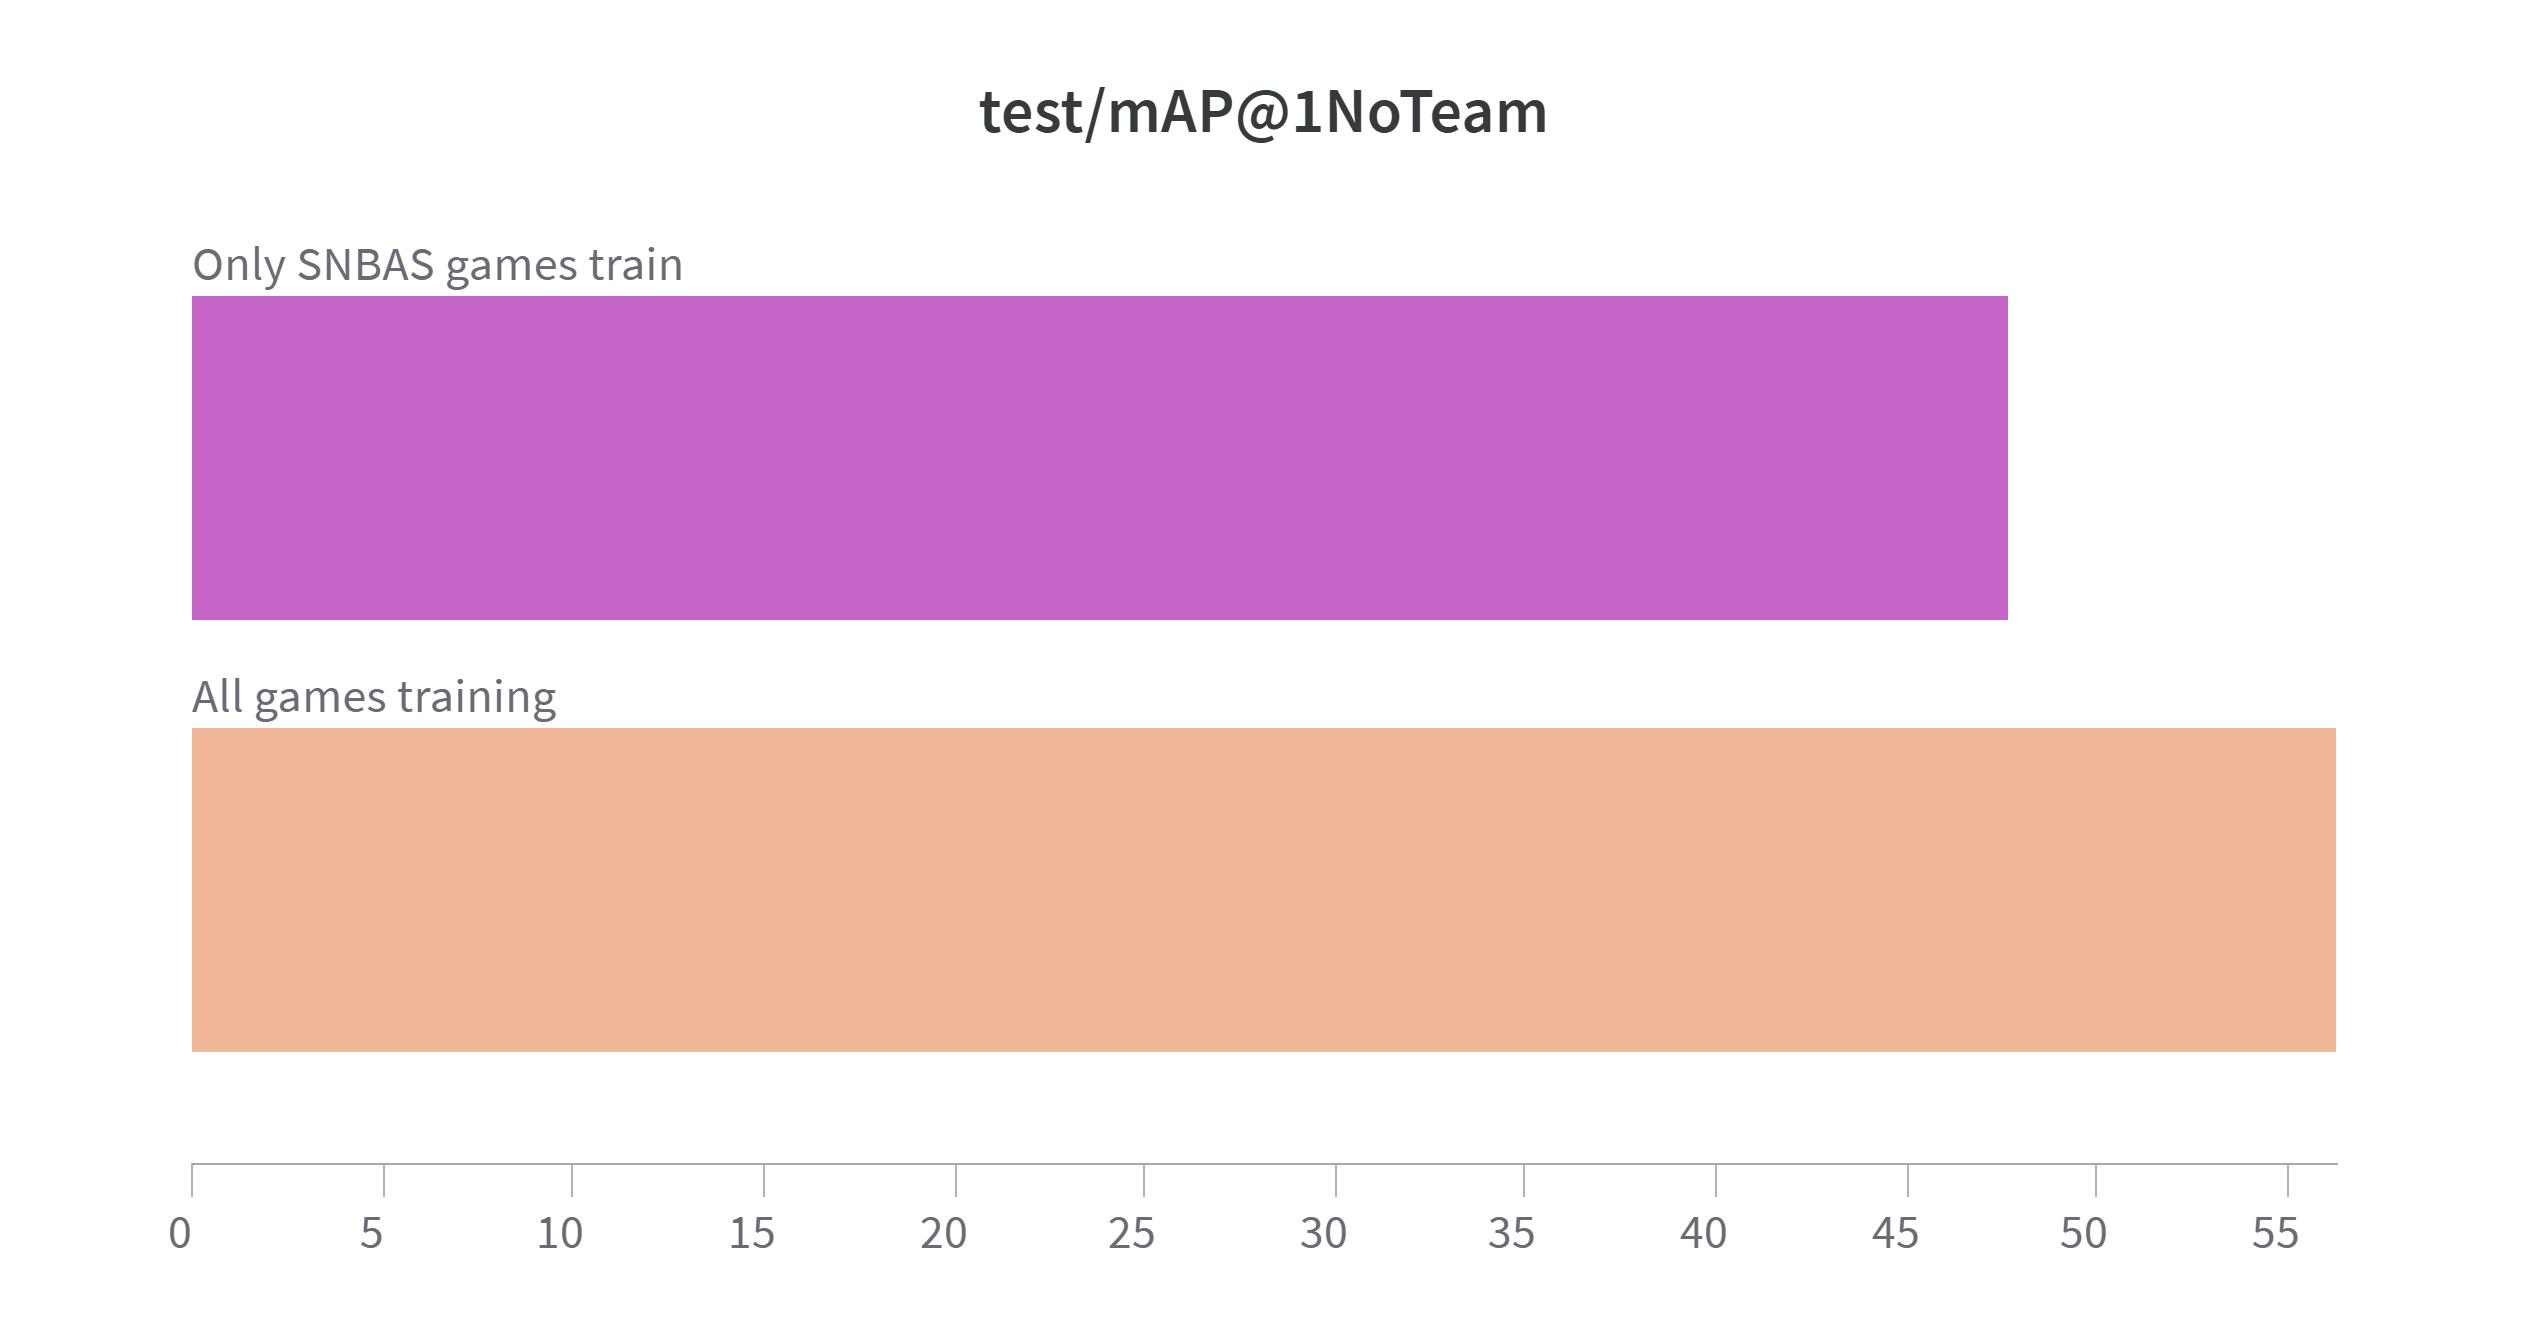
\includegraphics[width=\linewidth]{figures/total_map_no_team.png}
    \caption{The \acrshort{snb} training achieved a $47.65\%$ accuracy, the full training achieved $56.26\%$ when ignoring team prediction. }
    \label{fig:tdeed_map_no_team}
  \end{subfigure}%
  \hspace*{\fill}   % maximize separation between the subfigures
  \begin{subfigure}{0.5\textwidth}
    \centering
    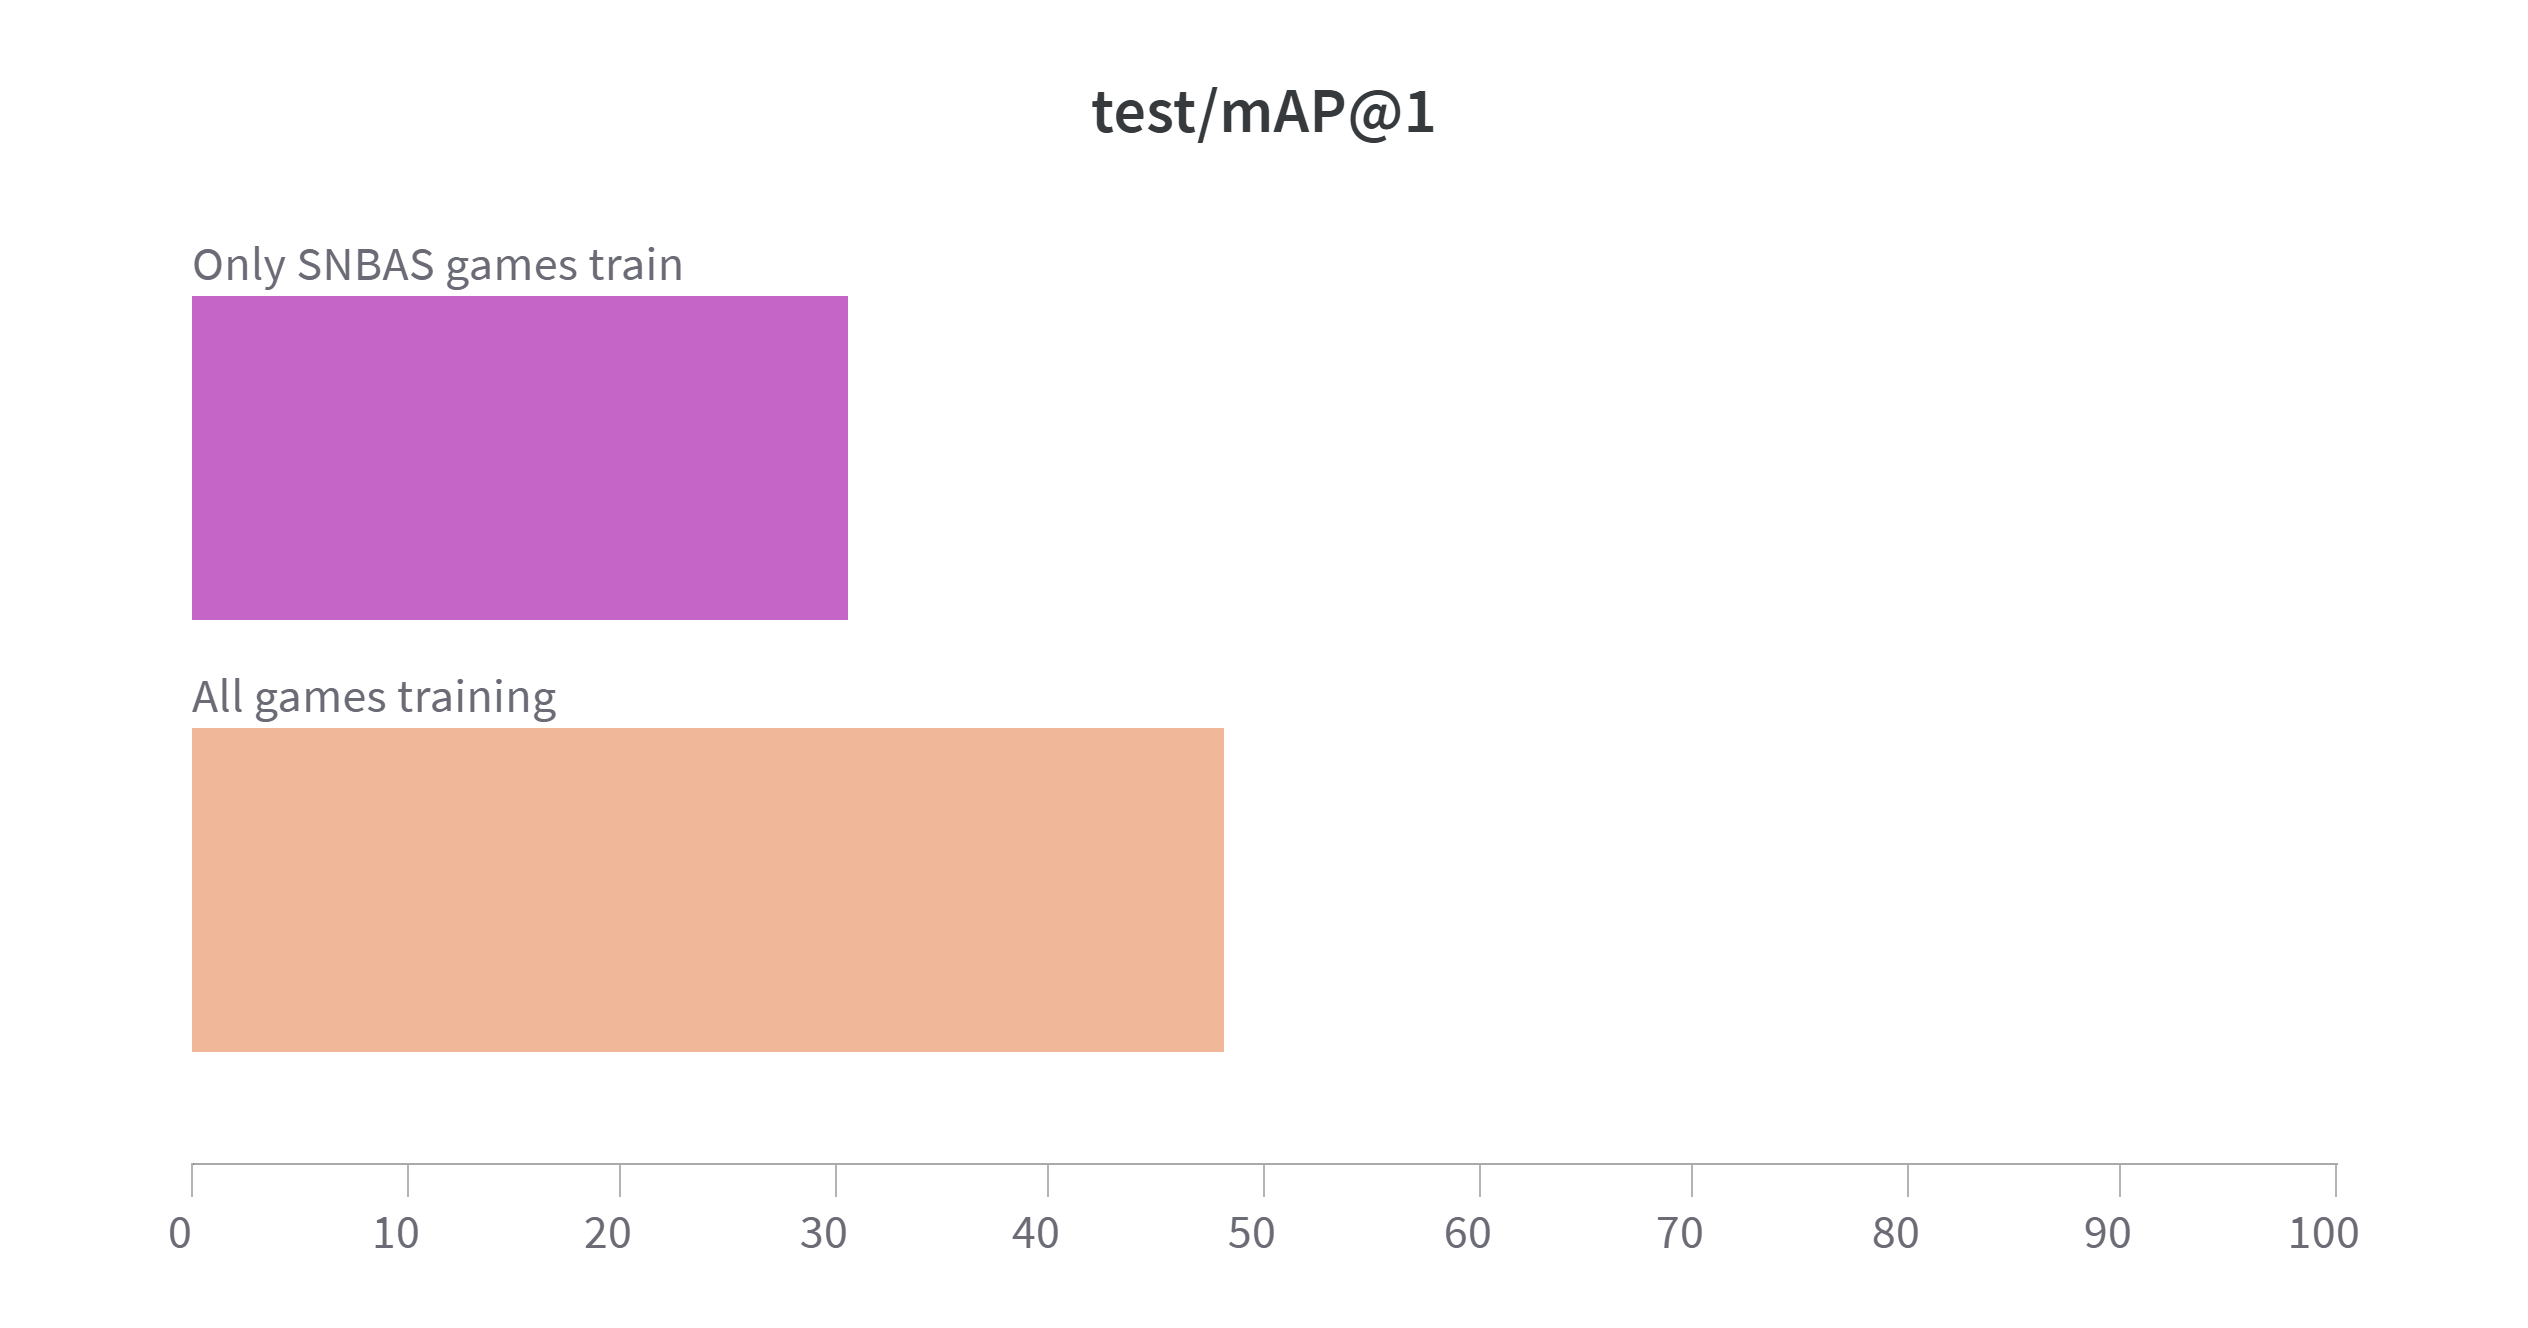
\includegraphics[width=\linewidth]{figures/total_map.png}
    \caption{The \acrshort{snb} and full model achived $30.62\%$ and $48.18\%$ respectively when  predicting teams. }
    \label{fig:map_team}
  \end{subfigure}%
  \hspace*{\fill}  
  \caption{The test-\acrshort{map} for the two models. The full training performed better in both categories, with and without team prediction. The difference was significant in both cases, but the difference increased when including the team predictions.}
  \label{fig:tdeed_map}
\end{figure}

\begin{figure}
    \centering
    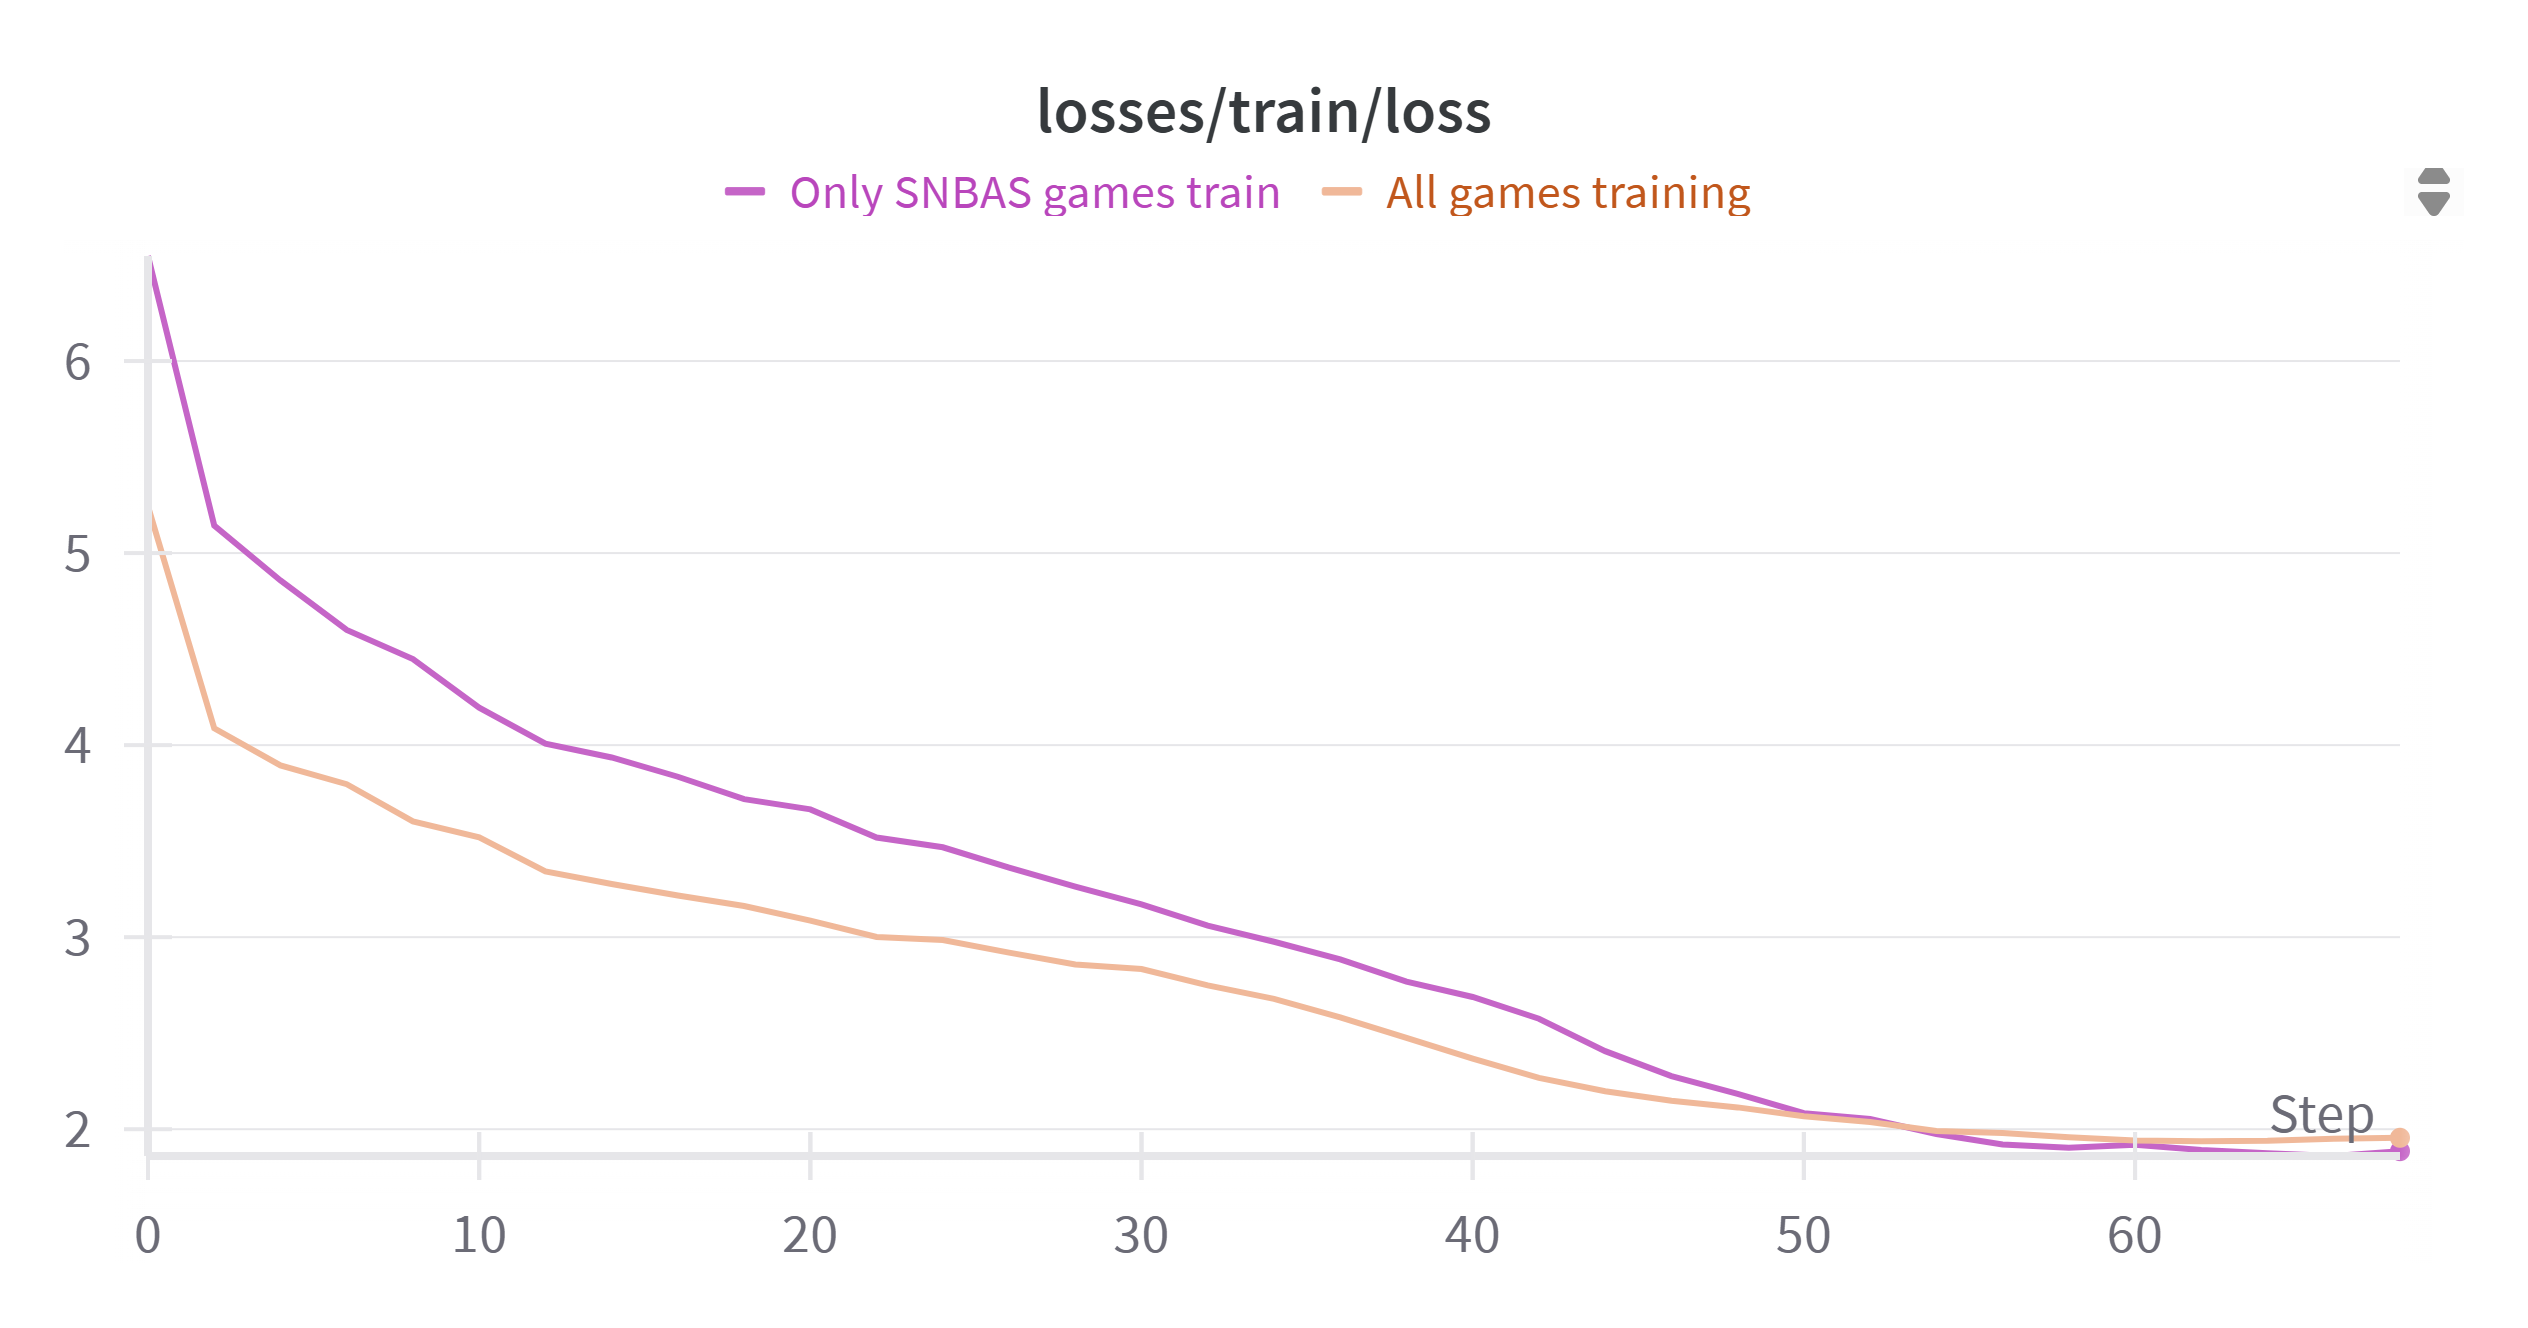
\includegraphics[width=0.5\linewidth]{figures/tdeed_train_loss.png}
    \caption{Training loss. The loss for all games is generally lower before both models converge at the same loss towards the end. }
    \label{fig:tdeed_train_loss}
\end{figure}

The results are showed in \cref{fig:500_7_val_compare,fig:tdeed_map_no_team,fig:map_team,fig:tdeed_train_loss} as direct comparisons. The result shows how the model with more training data performs better in all metrics, even though it is in another annotation format. The biggest difference comes when predicting the team, class, and time in \cref{fig:tdeed_map_no_team}.

\subsection{Discussion}
\label{ssec:ex5_discussion}



The most evident result is that the \acrshort{tdeed} model trained with more data (507 videos, "joint training") significantly outperforms the model trained only on \acrshort{snb} games. The performance gains align with general machine learning principles that more data yields better performance. The substantial jump shown in \cref{fig:tdeed_map} shows how the model trained on more data performs significantly better in the most complex task. All reported metrics report substantially better performance for the bigger model. 



Interestingly, the difference increases when adding the team's prediction. The large old dataset does not have annotations for teams. This signals that the model learns useful features for determining teams from just looking at games. This ability is extended to the realm where team matters. The difference in \acrshort{map} is doubled when adding team prediction, which shows the importance. Without targeted experiments, it is difficult to isolate where exactly the difference comes from.  




While the range of event types is different for the datasets, the information about events is more detailed. The belief is that the model uses game context to predict events. As discussed \todo{can''t find where rn} before, football actions are highly dependent on what action occurred before and what action will occur next. 



The fact that both models eventually converge to a similar loss suggests that, given enough training, both can fit their respective training datasets similarly. However, the initial lower loss for the model with more data suggests it gets a "head start" in this fitting process, likely due to the increased volume and richness of information available from the outset. The difference in validation and test scores underlines the idea of the richer context learned from the larger dataset. The model has better generalization. 


Experiment 5 aligns with the philosophy behind pre-training and transfer learning. Large-scale data helps build better, more generalizable models. While reaching the same loss on the training data, the validation scores are much better for the better-trained model, which proves its generalizability. Training in the football domain favors quantity and diversity, even with some annotation inconsistencies or variations in depth, over smaller, perfectly tailored datasets.


\section{Experiment 6: Testing validation stride and postprocessing of \acrshort{tdeed}}
\label{sec:experiment_6}

This experiment is motivated by earlier results, which suggested that postprocessing steps could be the cause of major performance improvements. 

\subsection{Setup}
\label{ssec:ex6_setup}
The setup is similar to \cref{sec:experiment_5}, where the small, new dataset is utilized. The only difference in these runs is:

\begin{itemize}
    \item \textbf{Stride} is set to one, not two, as in the baseline.
    \item \textbf{Postprocessing} is disabled, the baseline uses \acrlong{snms}.
\end{itemize}

\subsection{Results}
\label{ssec:ex6_results}

\begin{figure}
    \centering
    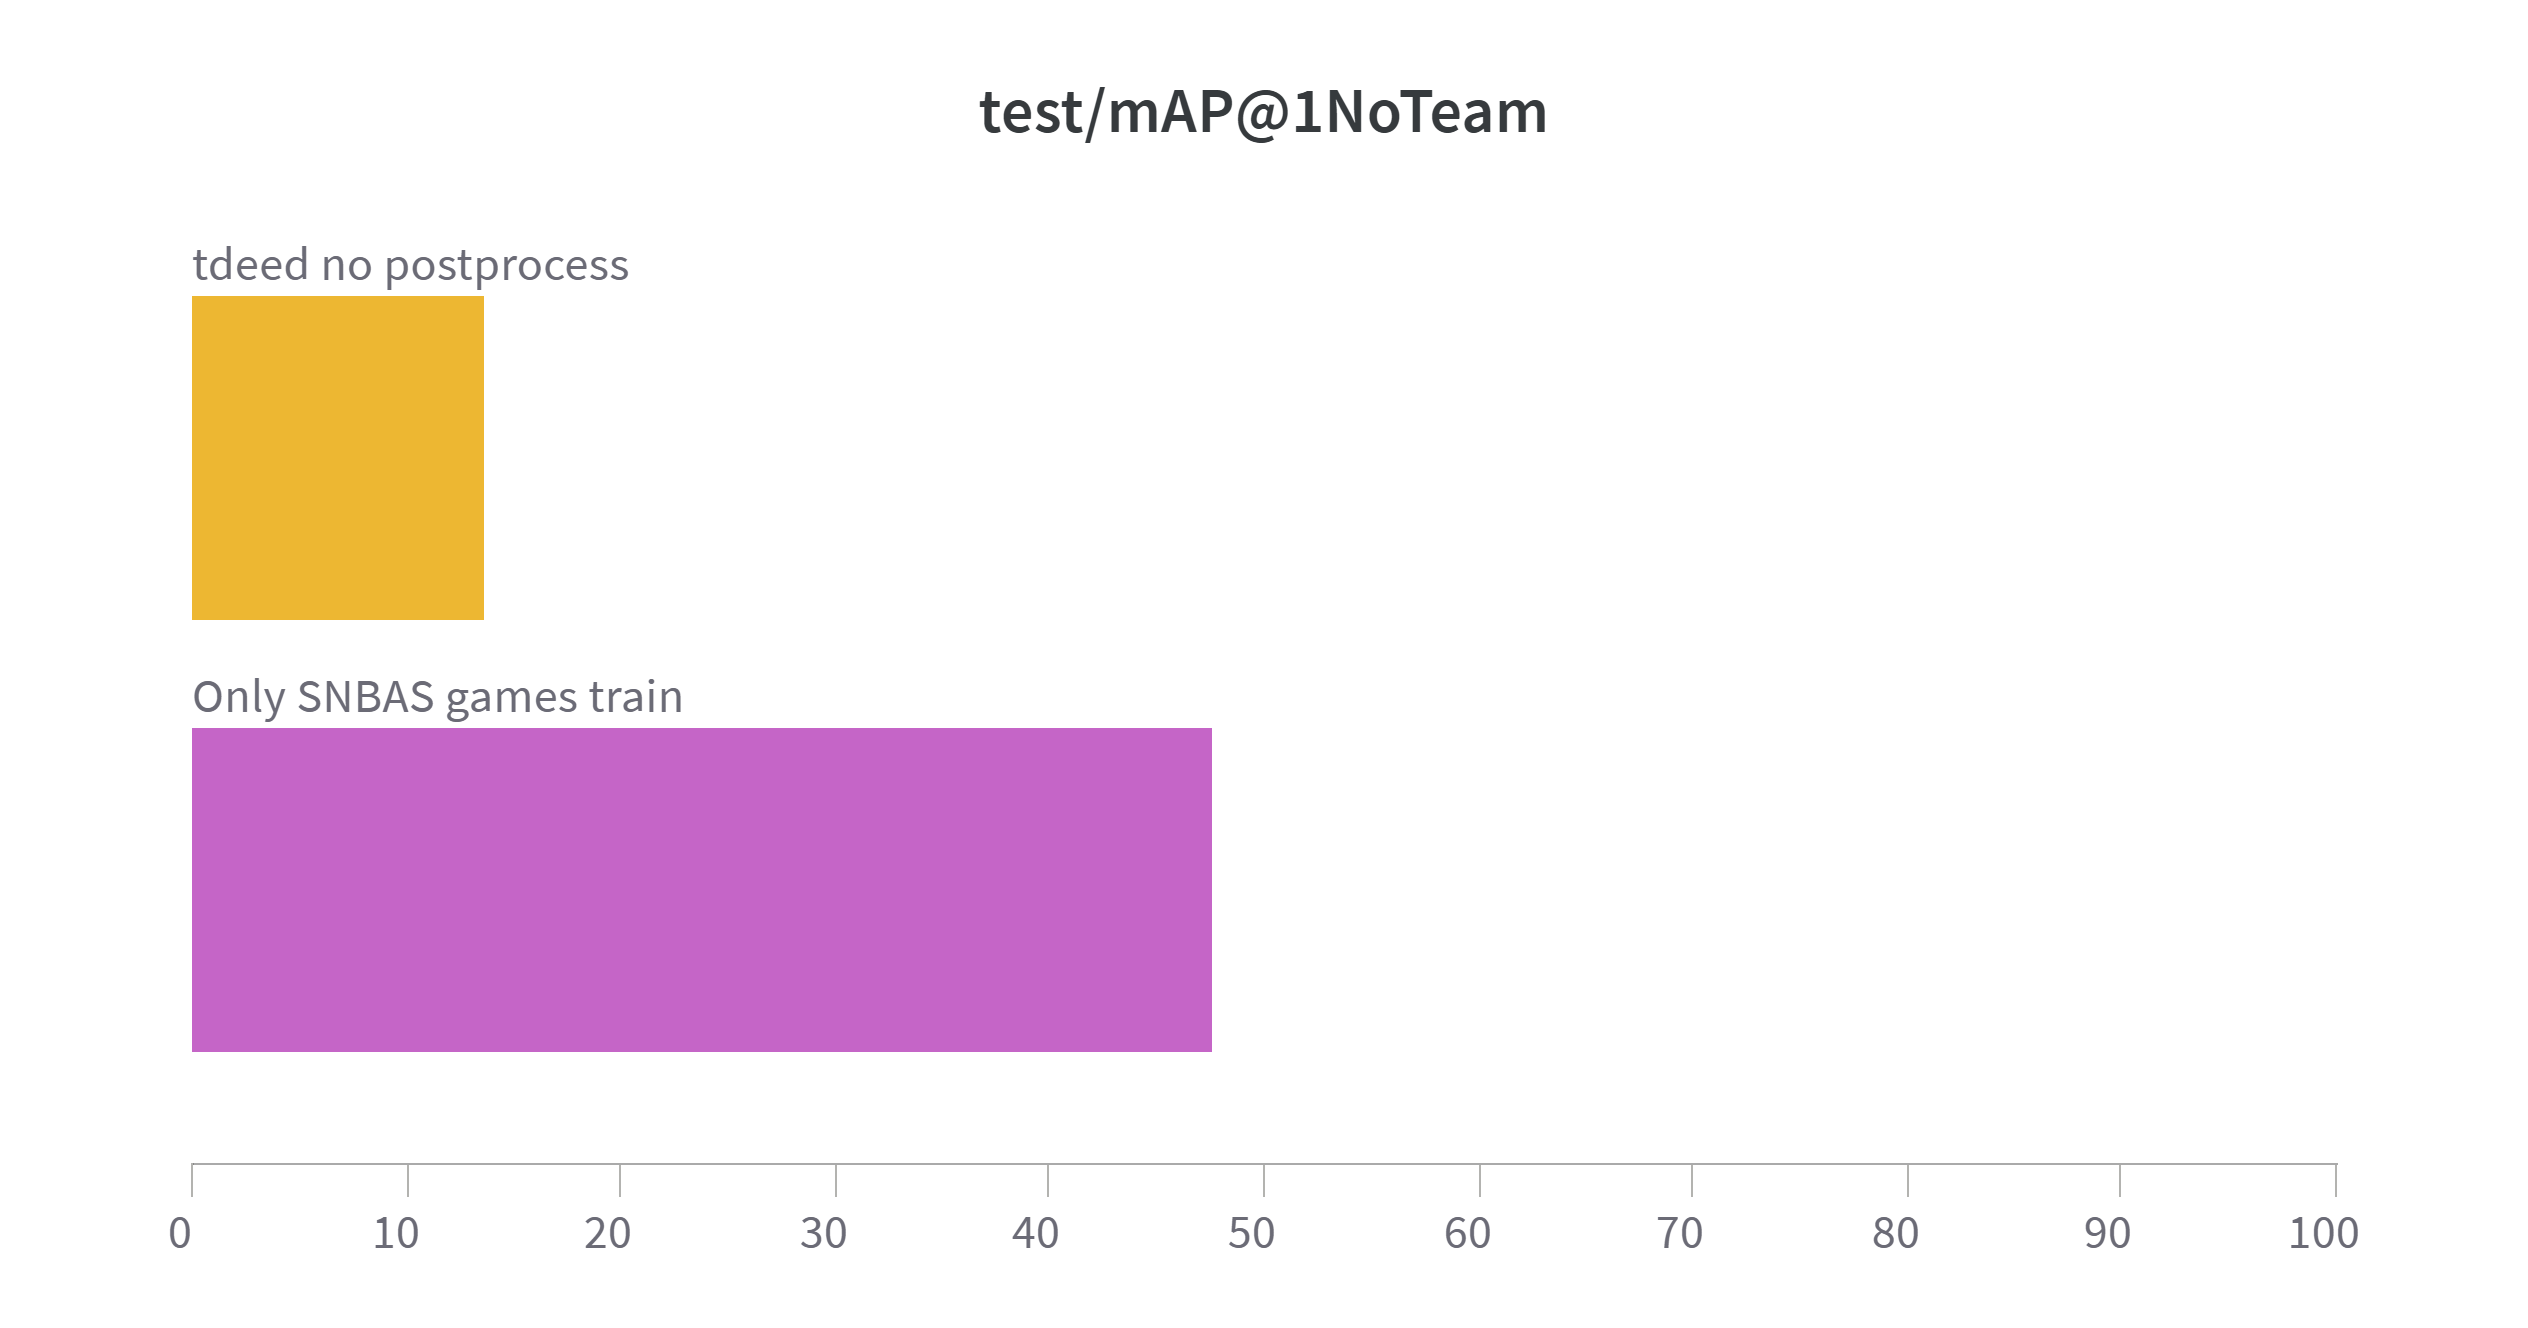
\includegraphics[width=0.75\linewidth]{figures/no_pprocess_test.png}
    \caption{Test results on the models. The figure shows the big impact of applying the postprocessing step. The test results of each model are $13.62\%$ and $47.65\%$, respectively. Both cases use $stride=1$.}
    \label{fig:ex6:no_pp_test}
\end{figure}

\begin{figure}
    \centering
    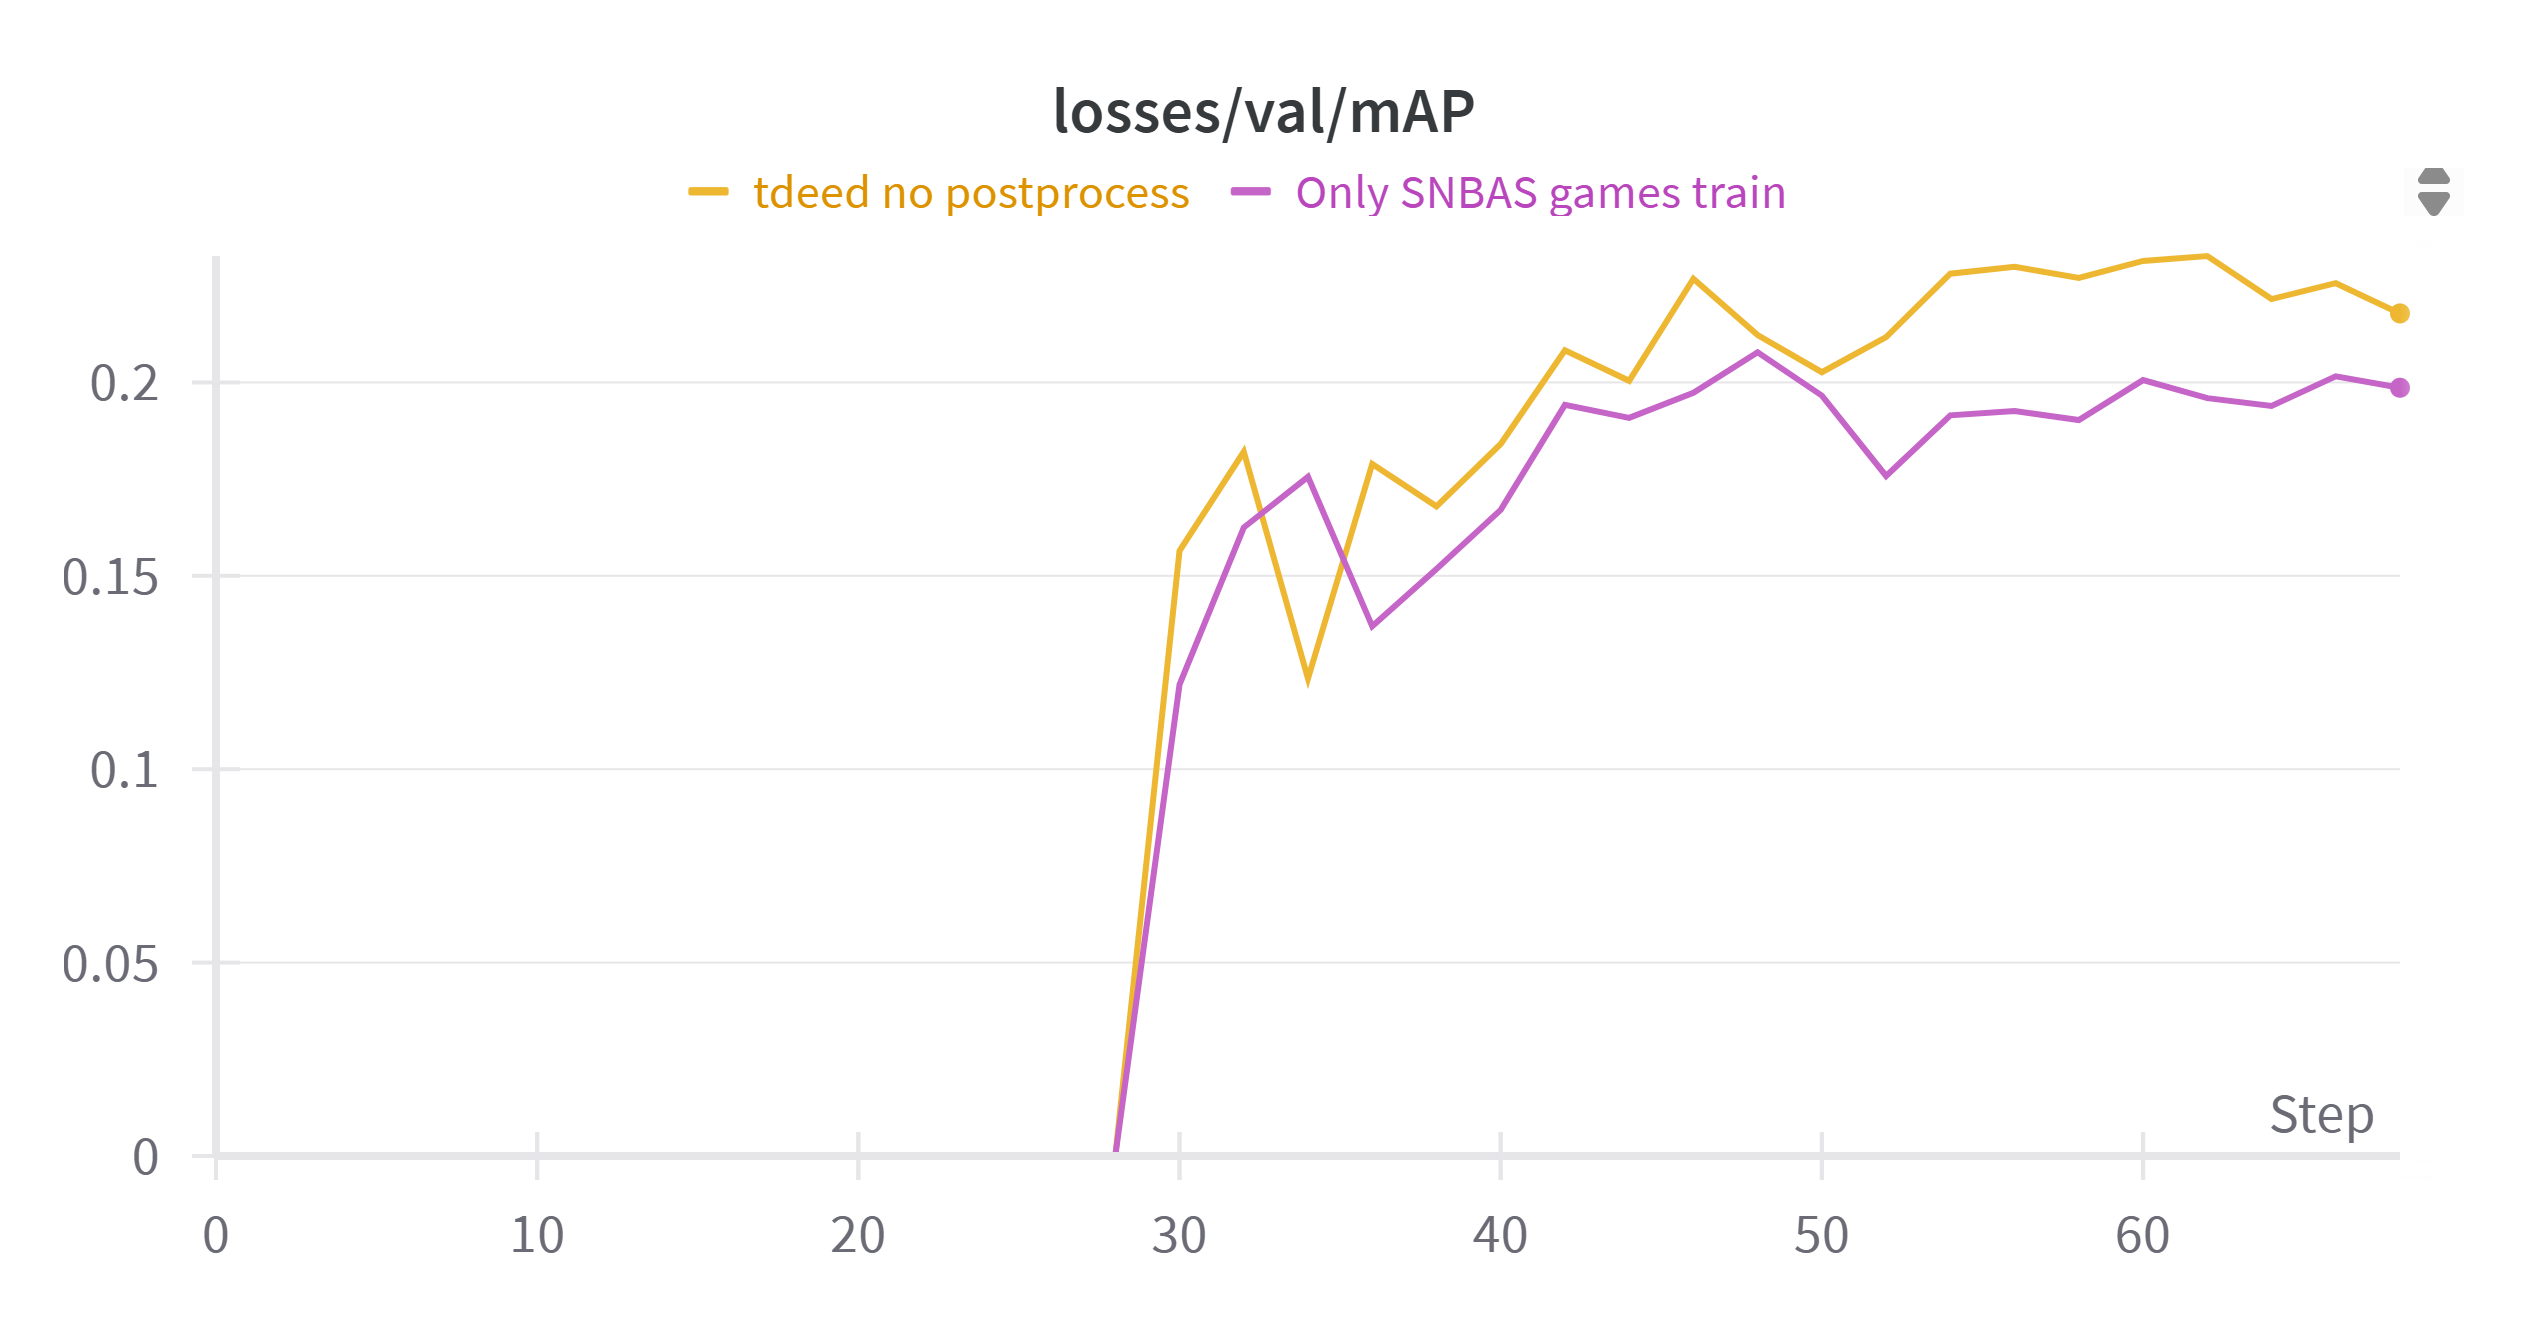
\includegraphics[width=0.75\linewidth]{figures/no_pprocess_val.png}
    \caption{The development of validation scores over the training session. After the first five validation epochs, where the results vary, the model with a lower validation stride is better. Their peaks at epoch 23 and 24, top out at $22.68\%$ and $20.78\%$. }
        \label{fig:ex6:no_pp_val}
\end{figure}

The validation differences were slight but notable. \cref{fig:ex6:no_pp_val} shows how the scores develop over time, and that their peaks vary not much in value. As seen in \cref{fig:ex6:no_pp_avg_val}, the difference in validation score increases as the training continues. 

\begin{figure}
    \centering
    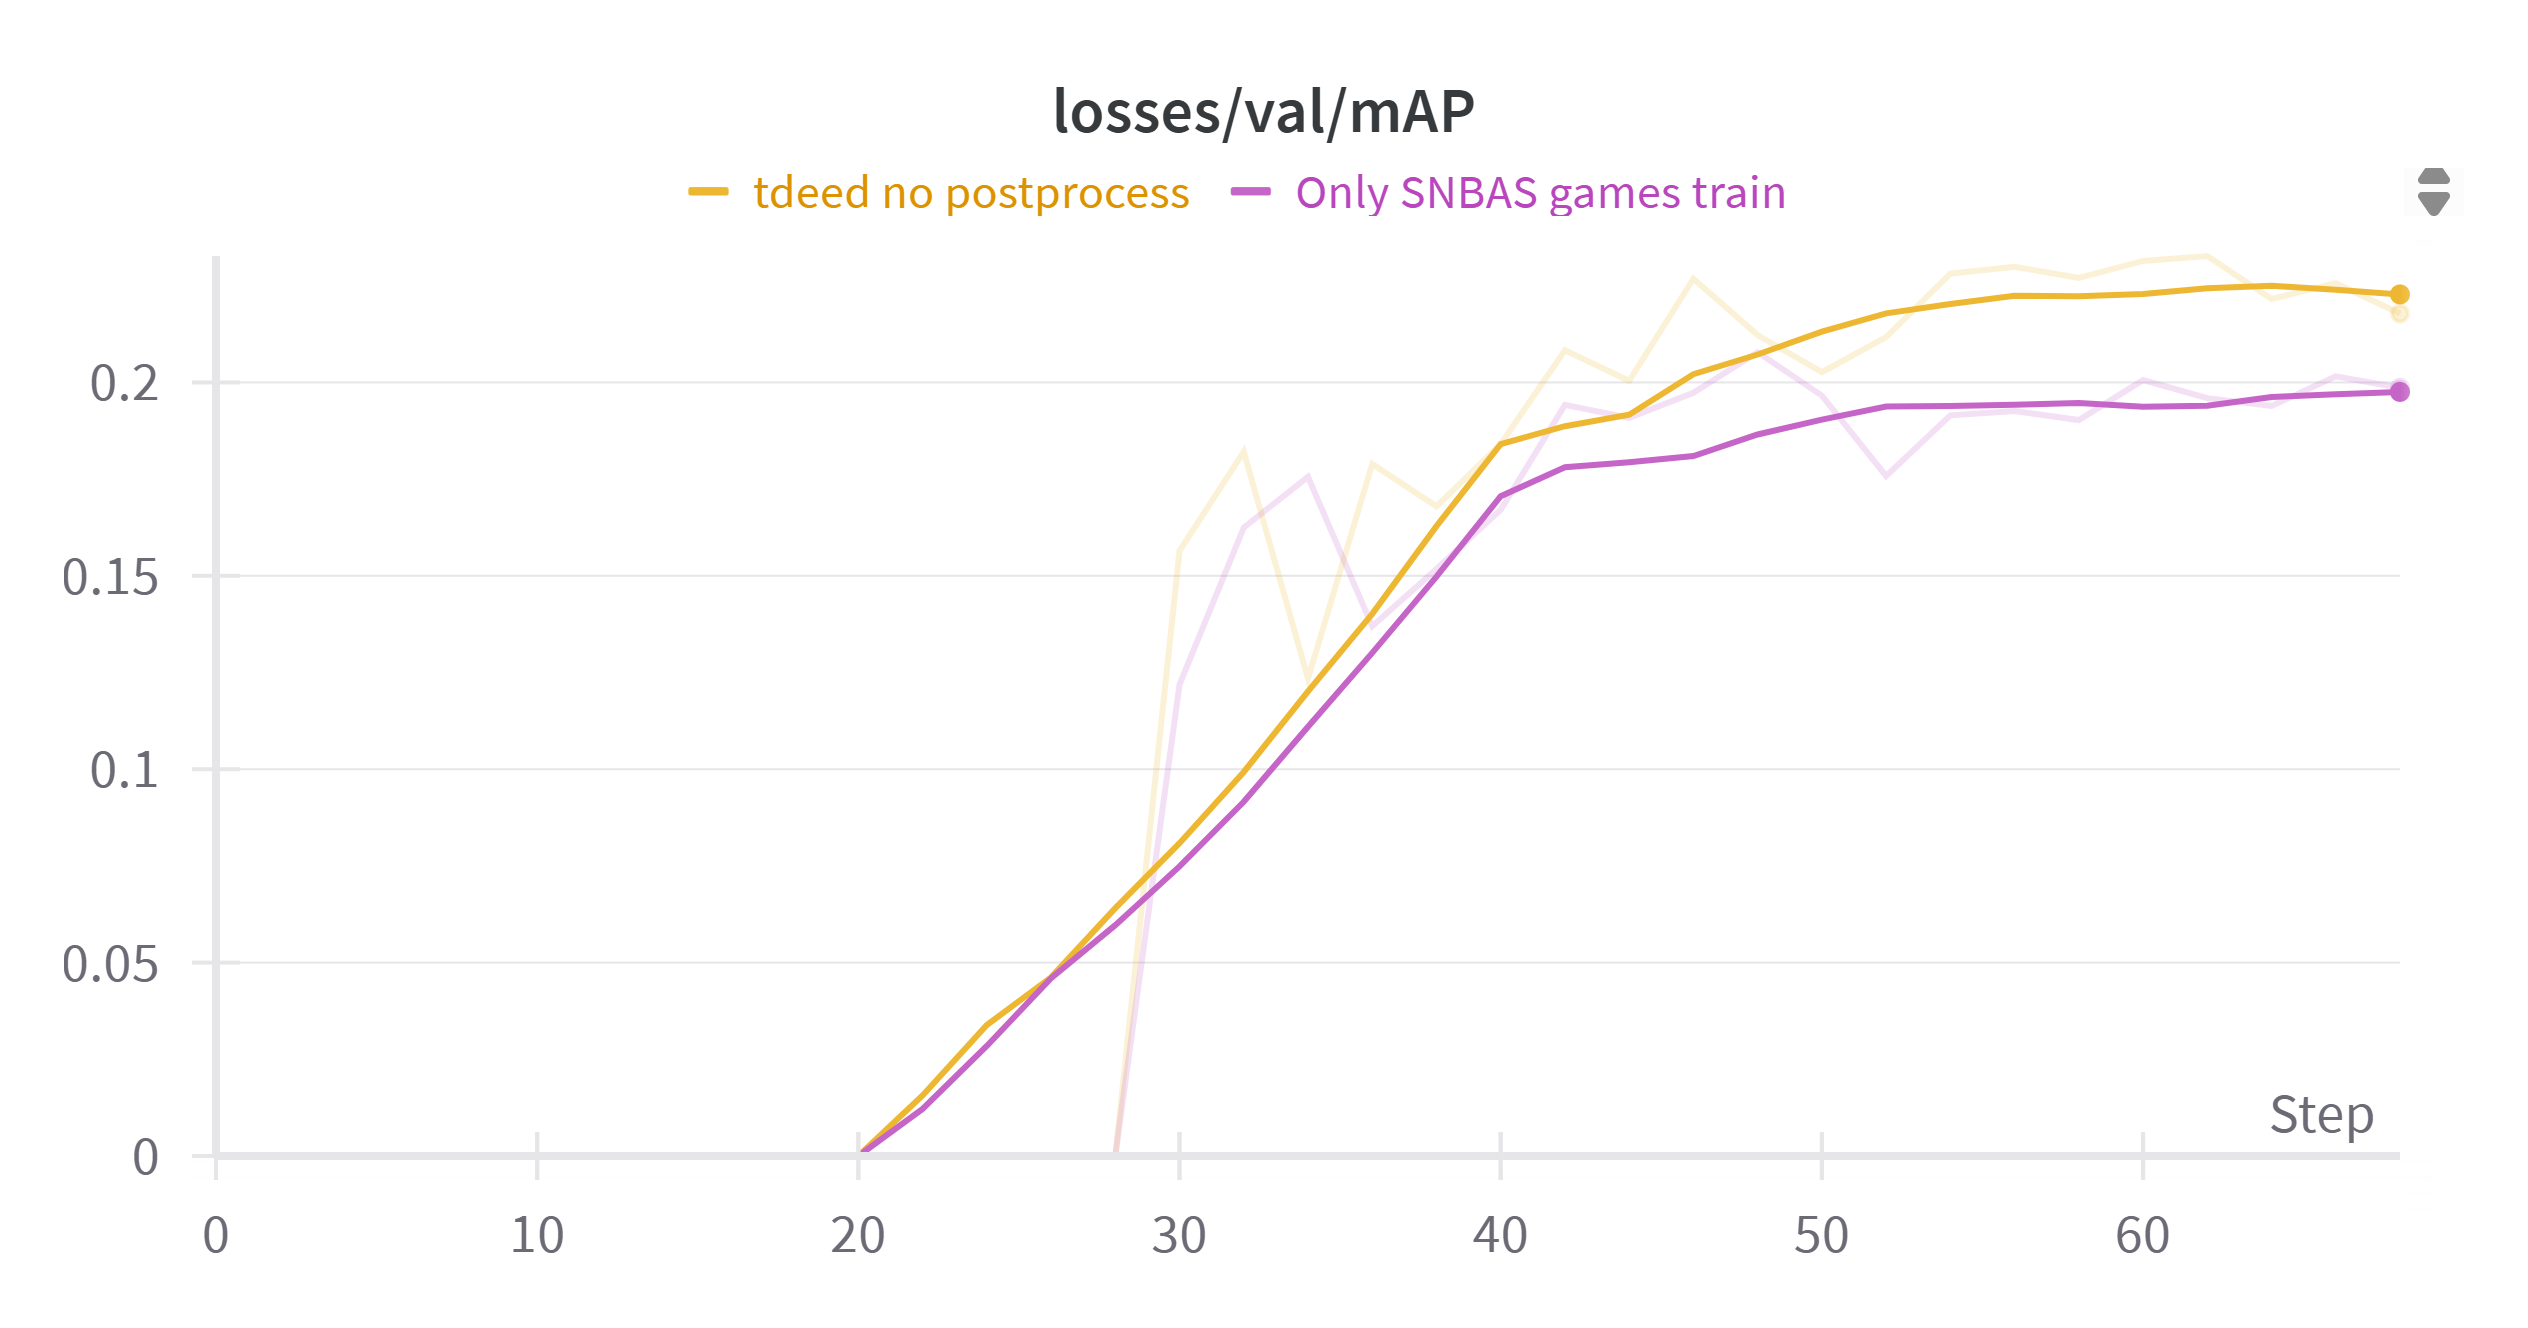
\includegraphics[width=0.75\linewidth]{figures/no_pprocess_avg_val.png}
    \caption{The same graph as in \cref{fig:ex6:no_pp_val}, but with the running average, not validation per epoch.}
    \label{fig:ex6:no_pp_avg_val}
\end{figure}

\begin{figure}
    \centering
    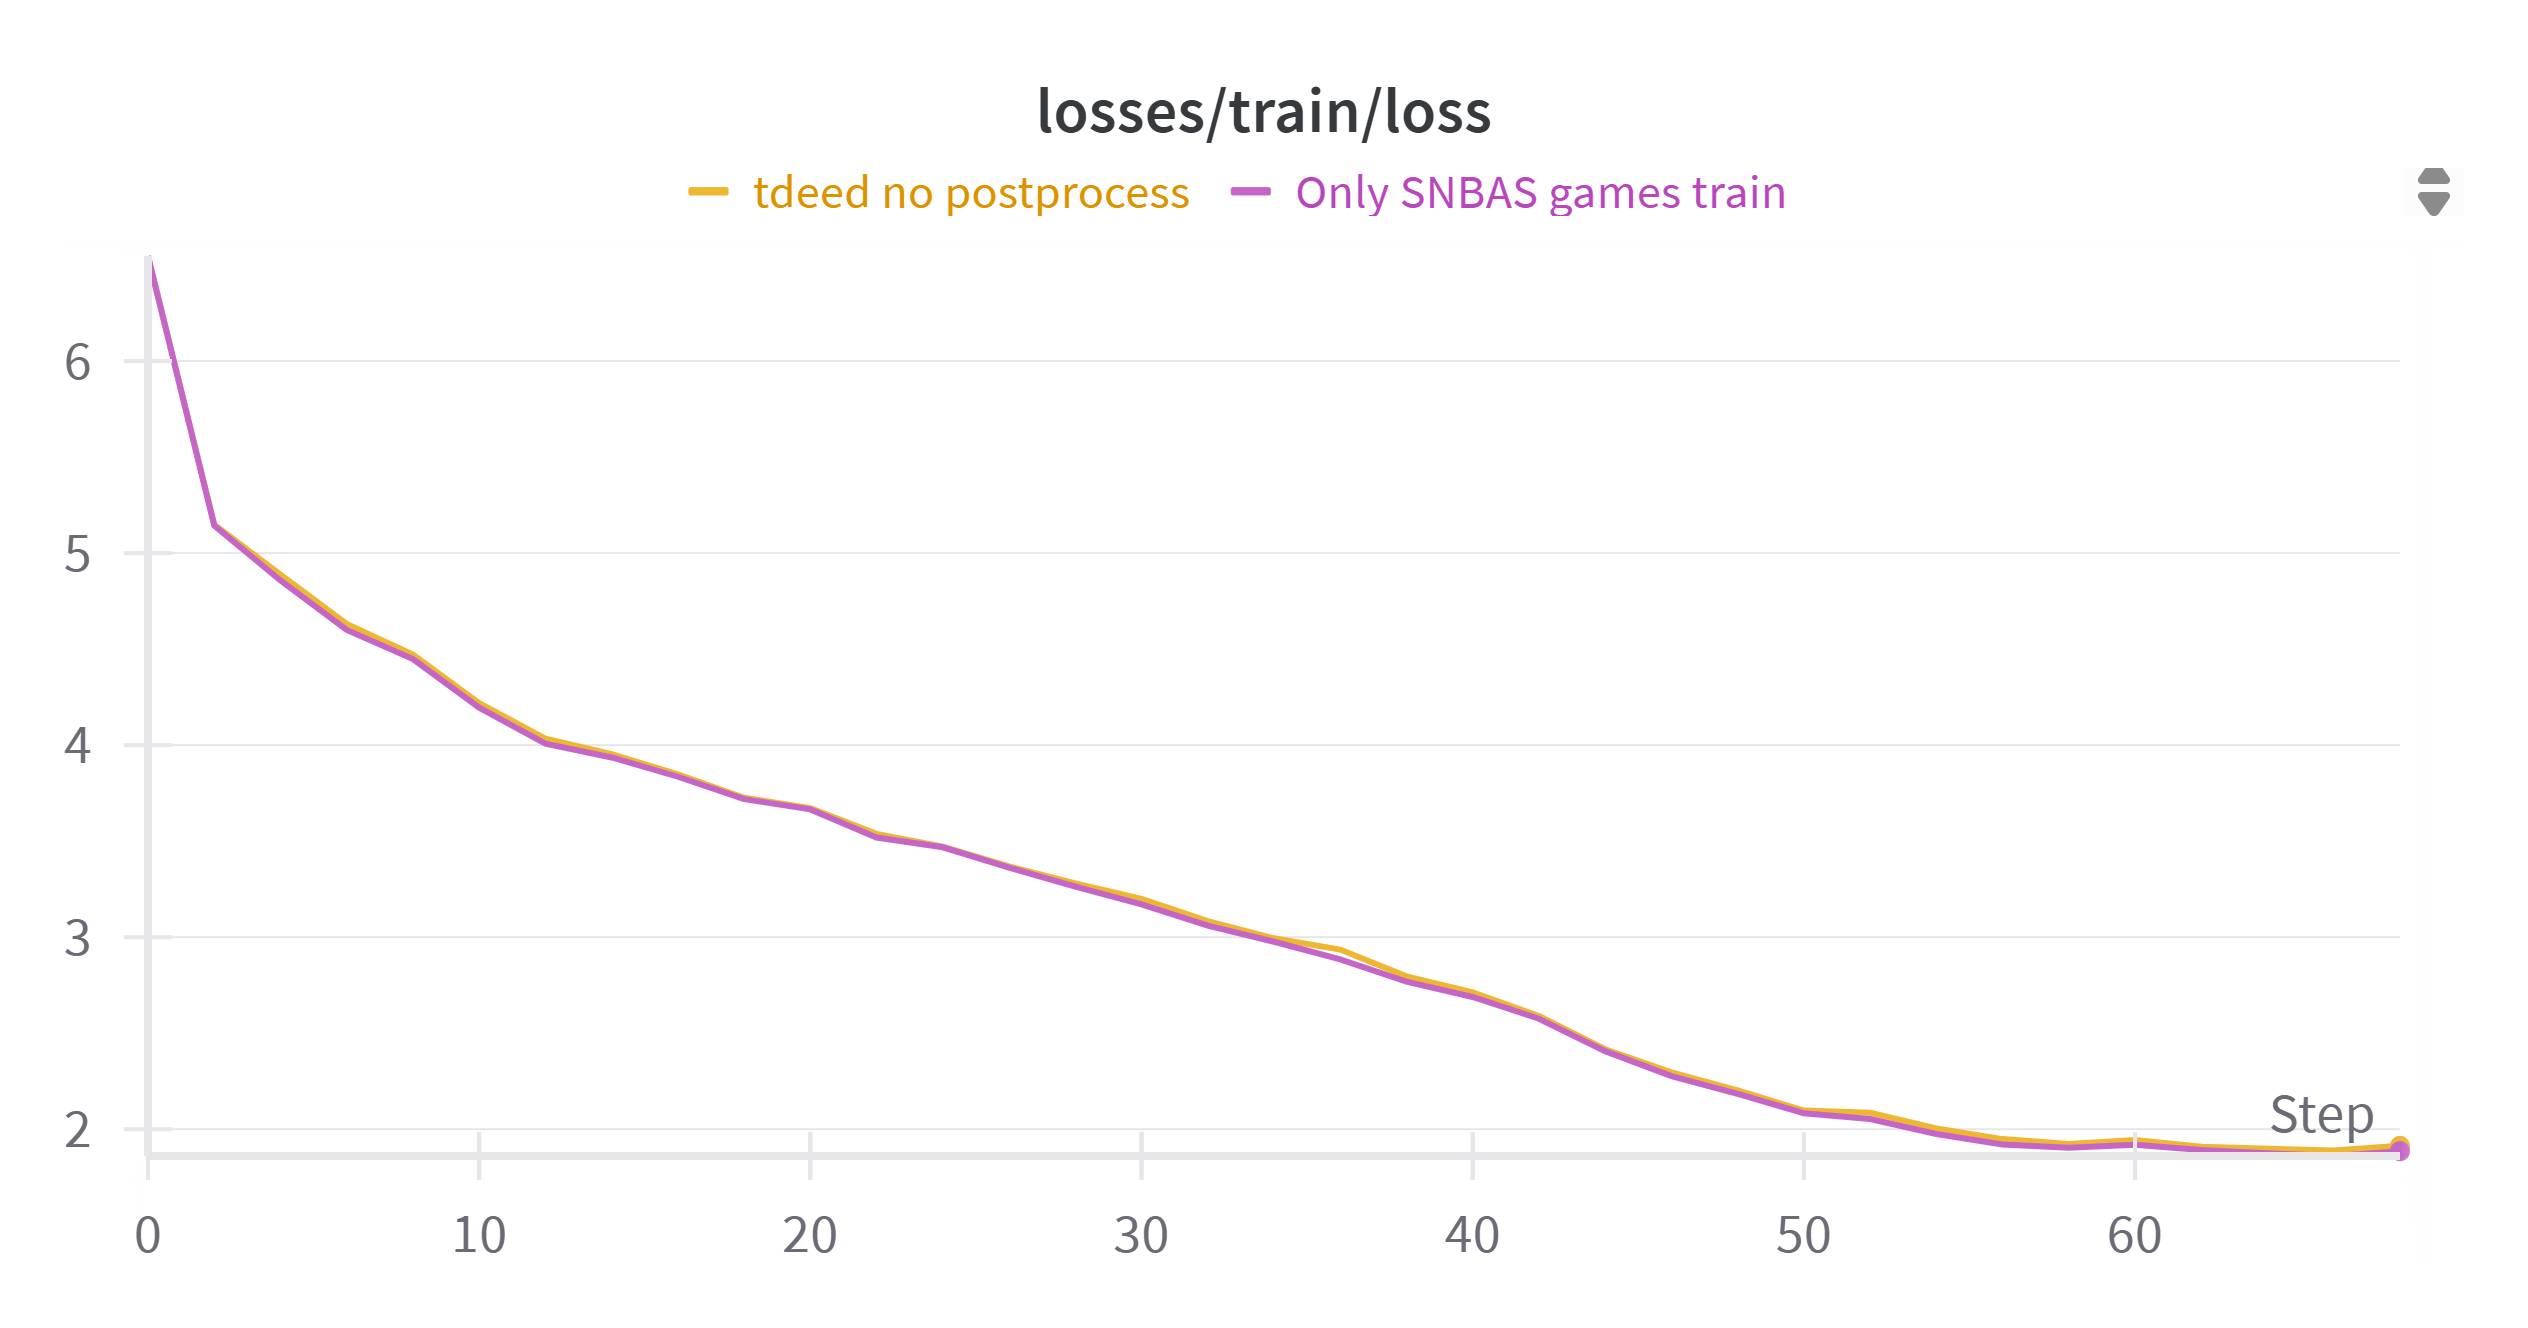
\includegraphics[width=0.75\linewidth]{figures/no_pprocess_loss.png}
    \caption{Loss scores for the two trainings. As expected, it is equal because only validation and test scores should vary.}
    \label{fig:ex6:no_pp_loss}
\end{figure}

The difference in test scores, \cref{fig:ex6:no_pp_test}, is significant. The model with postprocessing performs more than three times as well as the no-postprocessing model. If one recalls \cref{fig:tdeed_map_no_team}, the difference to the training model on the full dataset is $42.64\%$. 

\subsection{Discussion}
\label{ssec:ex6_discussion}


\acrfull{snms} is critical for \acrshort{tdeed}'s performance because the raw output likely contains many redundant and overlapping detections for the same event. The drop off when removing \acrshort{snms} is massive. Experiment 6 provides evidence that the validation score in Experiment 1 was significantly tampered with by the lack of \acrshort{snms}. The validation scores can not be directly compared from raw \acrshort{tdeed} to \acrshort{vms}. 

I did not expect the significance of the postprocessing to be as considerable as it was, and subsequently, the impact of the validation step to be so little. The importance could be greater if the model did not provide as many redundant, overlapping predictions. There is an increase from $stride=2$ to $stride=1$, an increase of $3\%$. A theory is that with such an acceptable margin of $\pm1s$, and the sheer number of predictions, more predictions fit within the constraints. There should not be any difference in the number of actions predicted, but in the temporal accuracy. 

This experiment confirms that \acrshort{snms} is the primary driver behind the increase from the validation to the test score. The stride change had a small but noticeable difference in validation. However, compared to the improvement from the postprocessing, the change was insignificant. After changing stride, the results were not comparable with \acrshort{vms}. 

The high impact from \acrshort{snms} could be because of the benchmark specificity. Because each event can only be assigned to one ground truth, many predictions around one ground truth will cause a low \acrlong{map}. For a detection system with $k$ redundant predictions per true object, the precision becomes:

\[P_{redundant} = \frac{TP}{TP + (k-1) \cdot TP} = \frac{1}{k}\]

This causes nonmax suppression to be necessary for a good result. \unsure{does this belong in method?} 

With validation results yielding different results, integrating postprocessing into the validation step must be discussed. Even if time-consuming, this step would be necessary to run a good hyperparameter search and get probable estimates of test results. Early stopping mechanisms based on validation scores might perform suboptimally. 

The findings and the clarification about the redundant positive predictions decrease the \acrshort{map} score of validation.

\section{Summary}

Experiment one compared \acrfull{vms} and \acrfull{tdeed}, finding that it was difficult to compare the two because of preprocessing. However, the model is likely more accurate with \acrshort{tdeed} achieving a higher test score than the validation score for \acrshort{vms}. No conclusion was reached on that. Experiment two confirmed \acrshort{vms}'s significant time complexity advantages, although a slow preprocessing timeline currently hinders its practical application. Pretraining proved helpful and should be applied to the \acrshort{vms} model. Using larger context vectors increased performance similarly. Future studies should focus on postprocessing techniques rather than hyperparameters. 
\chapter{Discussion}
\label{chap:discussion}

\section{Addressing the Research Questions Based on the Experiments}
\info{Quantitative results vs. baselines}
\info{Ablations on clip length, masking ratio, MAMBA variants}
\info{Error analysis / qualitative examples}


\subsection{\textbf{RQ1}:
How does the accuracy of the masked-autoencoder and mamba temporal action spotting model compare to existing \acrlong{sota} methods on the SoccerNet benchmark?}

With the current experiments, it is difficult to come to a clear conclusion on which model is better. Results indicate that \acrfull{tdeed} performs better, with \acrshort{vms} not living up to standards. This conclusion is reached by looking at the drop between validation, found in \cref{fig:ex6:no_pp_val}, and its test results shown in \cref{fig:ex6:no_pp_test}. The test results are significantly lower than the validation epoch. Therefore, looking at \cref{tab:results_ex1}, where the test results of \acrshort{tdeed} outperform the validation results found in \acrshort{vms}. It is inferred that the real validation using postprocessing would significantly outperform the \acrshort{vms}. 

This does not tell the true story. 

haven't done justice to the comparison


\subsection{RQ2:} 
What are the model’s inference speed and computational requirements compared to T-DEED?

add video-mae to the time is fair, as it contributes to the results

inference with tdeed much faster because of videomae before mamba


\subsection{RQ3:}
Which types of adaptation can be made to the MAMBA model to increase its precision?

Hyperparameters were configured from before, quite well. 
They might be suited to the feature extracted and not mamba directly. 
future Experiment with this


plot to check if it predicts equal amount of actions at all times, eg doesnt ignore first and last second 

\section{Limitations}
didnt fine tune the feature extractor
didnt test on rbk data
no pretraining
1 second fail margin of sn doesnt apply to actions in edge cases, but they are stricter. 
skewed distribution of events, even full tdeed training cant predict goal with correct team

\section{Reflections}
mamba should be explored more in the sports action recognition based on litareture review and results. 
a lot of time was spent debugging and setting up the project to run with mamba. 
registered for the competition
asked for too little help. didnt use either github nor discord nor supervisors very much
should have designed a math formula for hyperparameter optimalization
had daily standups with myself, those were useful. especially to see what took a lot of time, what blocked me.
trying to make my own model from scratch was a waste of time
could it be erronous that all clips have the same size because of the last clips in each game not having
i want to build my own simpler model :) and understand the whole process
significant impact of postprocessing in tdeed
understand more about suppression with the map score
vms runs on any GPU, but tdeed needs a lot of memory and only runs on premium GPUs.
could sit here and add up increases and pretend it would be the predicted results of an increased, but no value without experiments
hard to say how much info is gained/lost from video mae

\section{Sustainability}
VideoMAE is not very good. MAMBA in itself is nice. if you calculate power. i can do something similar with power need as done in visual intelligence, but i do not have all the data in wandb now. 
\chapter{Conclusion and Future Work}
\label{chap:conclusion}

\section{Conclusion}
\label{sec:conclusion}
This thesis investigated the usefulness of the Mamba-based \acrfull{vms} model for temporal action spotting in football videos. It compared the model with the \acrfull{sota} \acrfull{tdeed} model on the SoccerNet benchmark. The research aimed to answer three primary questions regarding the accuracy, computational efficiency, and potential adaptations for the \acrshort{vms} model.

Regarding accuracy (RQ1), a definitive comparison proved challenging. The \acrshort{tdeed} model achieved a test \acrshort{map}@50 of 47.65\%, while the \acrshort{vms} model obtained a validation \acrshort{map}@50 of 43.62\%. However, the absence of a test \acrshort{map}@50 for \acrshort{vms} and significant differences in evaluation protocols, particularly the critical role of \acrfull{snms} postprocessing for \acrshort{tdeed} (Experiment 6), hindered a direct, like-for-like comparison. The inherent differences between \acrshort{vms} as an action localization framework and \acrshort{tdeed} as an action spotting model further complicated this assessment.

In terms of inference speed and computational requirements (RQ2, Experiment 2), the \acrshort{vms} model demonstrated substantially faster training times (43 minutes vs. over 54 hours for \acrshort{tdeed}) and significantly lower computational demands. \acrshort{vms} was capable of running on less powerful \acrshort{gpu}s. While \acrshort{vms}'s raw inference speed is exceptionally high, its current reliance on a lengthy \acrshort{vmae} preprocessing pipeline (342 minutes per game) makes \acrshort{tdeed} (18 minutes total per game) more practical for end-to-end processing of unseen videos.

Examining adaptations to improve \acrshort{vms}'s precision (RQ3) reveals several promising avenues for improvement. Increasing feature dimensionality from 1408 to 3200 yielded a 3.2\% absolute \acrshort{map} gain on THUMOS-14 (Experiment 3), suggesting similar benefits for football data. Experiment 5, which showed \acrshort{tdeed}'s performance improvement with more extensive pretraining, implies that pretraining the \acrshort{vms} model would increase its result. Fine-tuning feature extractors, such as \acrshort{vmae}, on domain-specific data could also benefit \acrshort{vms}. Furthermore, the significant impact of postprocessing on \acrshort{tdeed} (Experiment 6) suggests that implementing robust postprocessing techniques, such as \acrshort{snms}, for \acrshort{vms} is a possible step for performance improvement. Hyperparameter optimization for \acrshort{vms} (Experiment 4) indicated that default parameters are relatively robust, with a lower learning rate showing some benefit, but extensive tuning yielded only marginal gains.

The \acrshort{s6} architecture within \acrshort{vms} did not unequivocally outperform the established \acrshort{tdeed} model in its current configuration for this specific task. However, its significantly reduced training time and computational footprint highlight its potential, particularly in resource-constrained environments or scenarios requiring frequent retraining. The primary limitations identified were the difficulties in direct metric comparison due to differing model paradigms and evaluation setups, as well as the bottleneck imposed by the \acrshort{vmae} feature extraction.

The findings suggest that the Mamba architecture is a promising direction for future work on video analysis, but not without further optimization and adaptation. The domain of football action spotting is a complex one, but there is no evidence that Mamba does not have huge potential. The work also highlighted sustainability considerations, favoring \acrshort{s6}'s efficiency, and noted the lack of gender diversity in the SoccerNet dataset, an area for future improvement in sports analytics.


\section{Future Work}
\label{sec:future_work}
Based on the findings and limitations identified in this thesis, I will propose new avenues of research. To further advance the capabilities of Mamba-based models for temporal action spotting in football, the following challenges should be addressed:

\subsection{Model Architecture and Adaptation}

\subsubsection{Refine \acrshort{vms} for Action Spotting:} 
Adapt the input and output layers of the \acrshort{vms} model. They should become more suited to the action spotting task rather than relying on conversion to its native temporal action localization framework. The challenge involves investigating how to represent and predict single-timestamp events effectively. Attacking this will allow for a fairer comparison to \acrshort{tdeed}

\subsubsection{End-to-End Training:} 
Explore end-to-end training of the \acrshort{vms} model with a learnable feature extractor. Reduce the reliance on fixed, pre-extracted features like \acrshort{vmae} and allow the feature extraction process to be optimized for the spotting task.

\subsection{Feature Representation}

\subsubsection{Optimize Feature Extraction for \acrshort{vms}:}
    \begin{itemize}
        \item \textbf{Reduce \acrshort{vmae} Preprocessing Time:} Investigate methods to significantly speed up the \acrshort{vmae} feature extraction pipeline, or explore lighter alternative feature extractors that maintain high descriptive power.
        \item \textbf{Fine-tune \acrshort{vmae} on Football Data:} Fine-tune the \acrshort{vmae} model on the SoccerNet dataset.
        \item \textbf{Study Masking Ratios:} Experiment with different masking ratios and strategies within \acrshort{vmae} if fine-tuning or retraining it. Optimize for the characteristics of football actions.
    \end{itemize}
    
\subsubsection{Higher-Dimensional and Alternative Features:} 
Systematically evaluate the impact of using higher-dimensional features (e.g., 3200-dimensional InternVideo features) with \acrshort{vms} on the SoccerNet dataset. Build on the promising results from THUMOS-14.

\subsubsection{Multi-modal Features:} 
Explore the incorporation of other modalities, such as audio features or player/ball tracking data, to enhance the input representation for the \acrshort{vms} model.

\subsection{Data Strategies and Handling}

\subsubsection{Address Skewed Event Distribution:} Develop and test strategies to mitigate the impact of highly skewed event distributions in the SoccerNet dataset.

\subsubsection{Dataset Expansion and Diversity:}
    \begin{itemize}
        \item \textbf{Create Labeled \acrfull{rbk} Dataset:} Undertake the creation and annotation of a dataset from \acrshort{rbk} data to enable model testing and fine-tuning on team-specific footage.
        \item \textbf{Incorporate Female Football Data:} Advocate for and utilize datasets that include female football games to improve model generalizability, address \acrshort{sdg} 5, and reduce potential biases. \acrshort{rbk} has a female team, and they probably record their games. 
    \end{itemize}
    
\subsubsection{Data Augmentation:} Develop and evaluate data augmentation techniques tailored explicitly to temporal action spotting in football videos to improve model robustness.

\subsubsection{Model Interpretability:} Apply interpretability techniques to understand what features and temporal patterns the \acrshort{vms} model learns to identify different football actions, particularly how the Mamba mechanism processes long-range dependencies.


\chapter*{\bibname}
\printbibliography[heading=none]

\appendix
\chapter{Sweeps}
\label{app:sweep}


\clearpage
\section{Sweep 1}
\label{app:sweep_1}
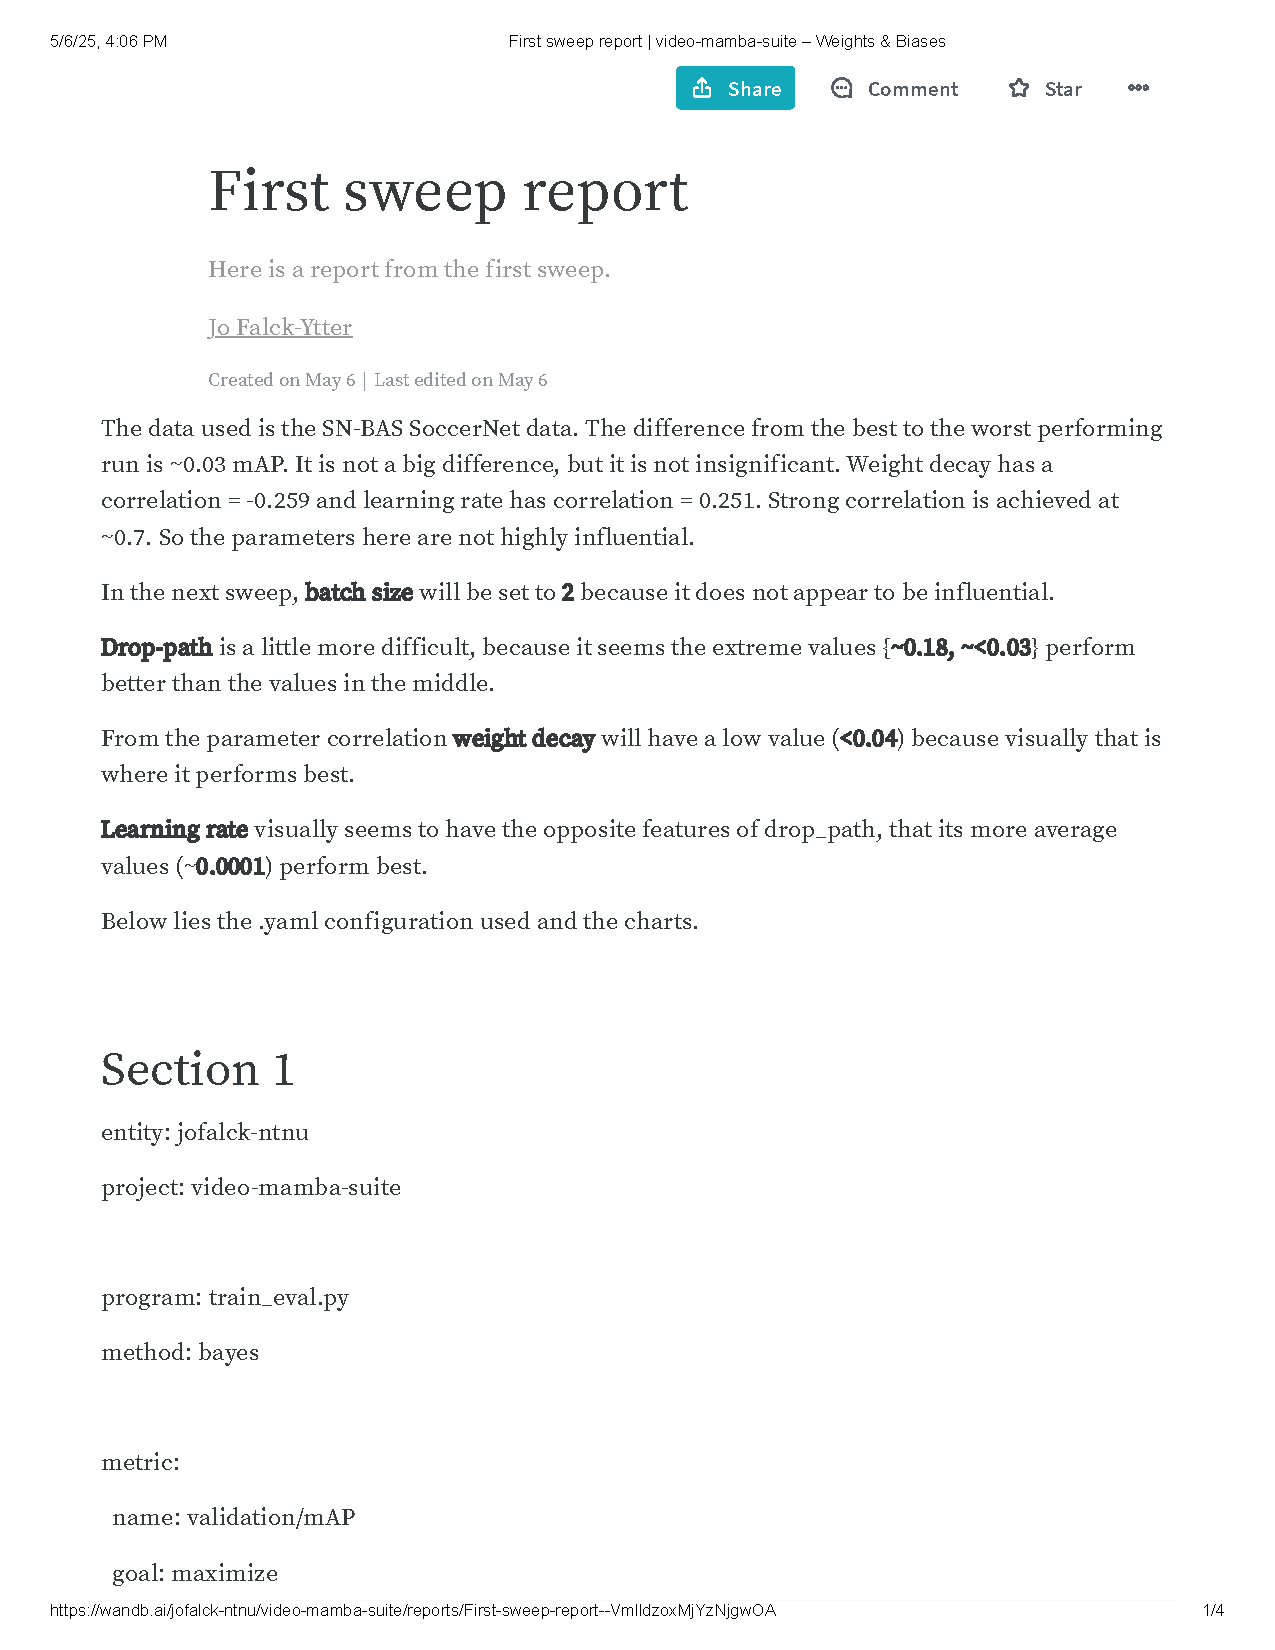
\includepdf[pages=-]{appendices/sweep1.pdf}

\clearpage
\section{Sweep 2}
\label{app:sweep_2}
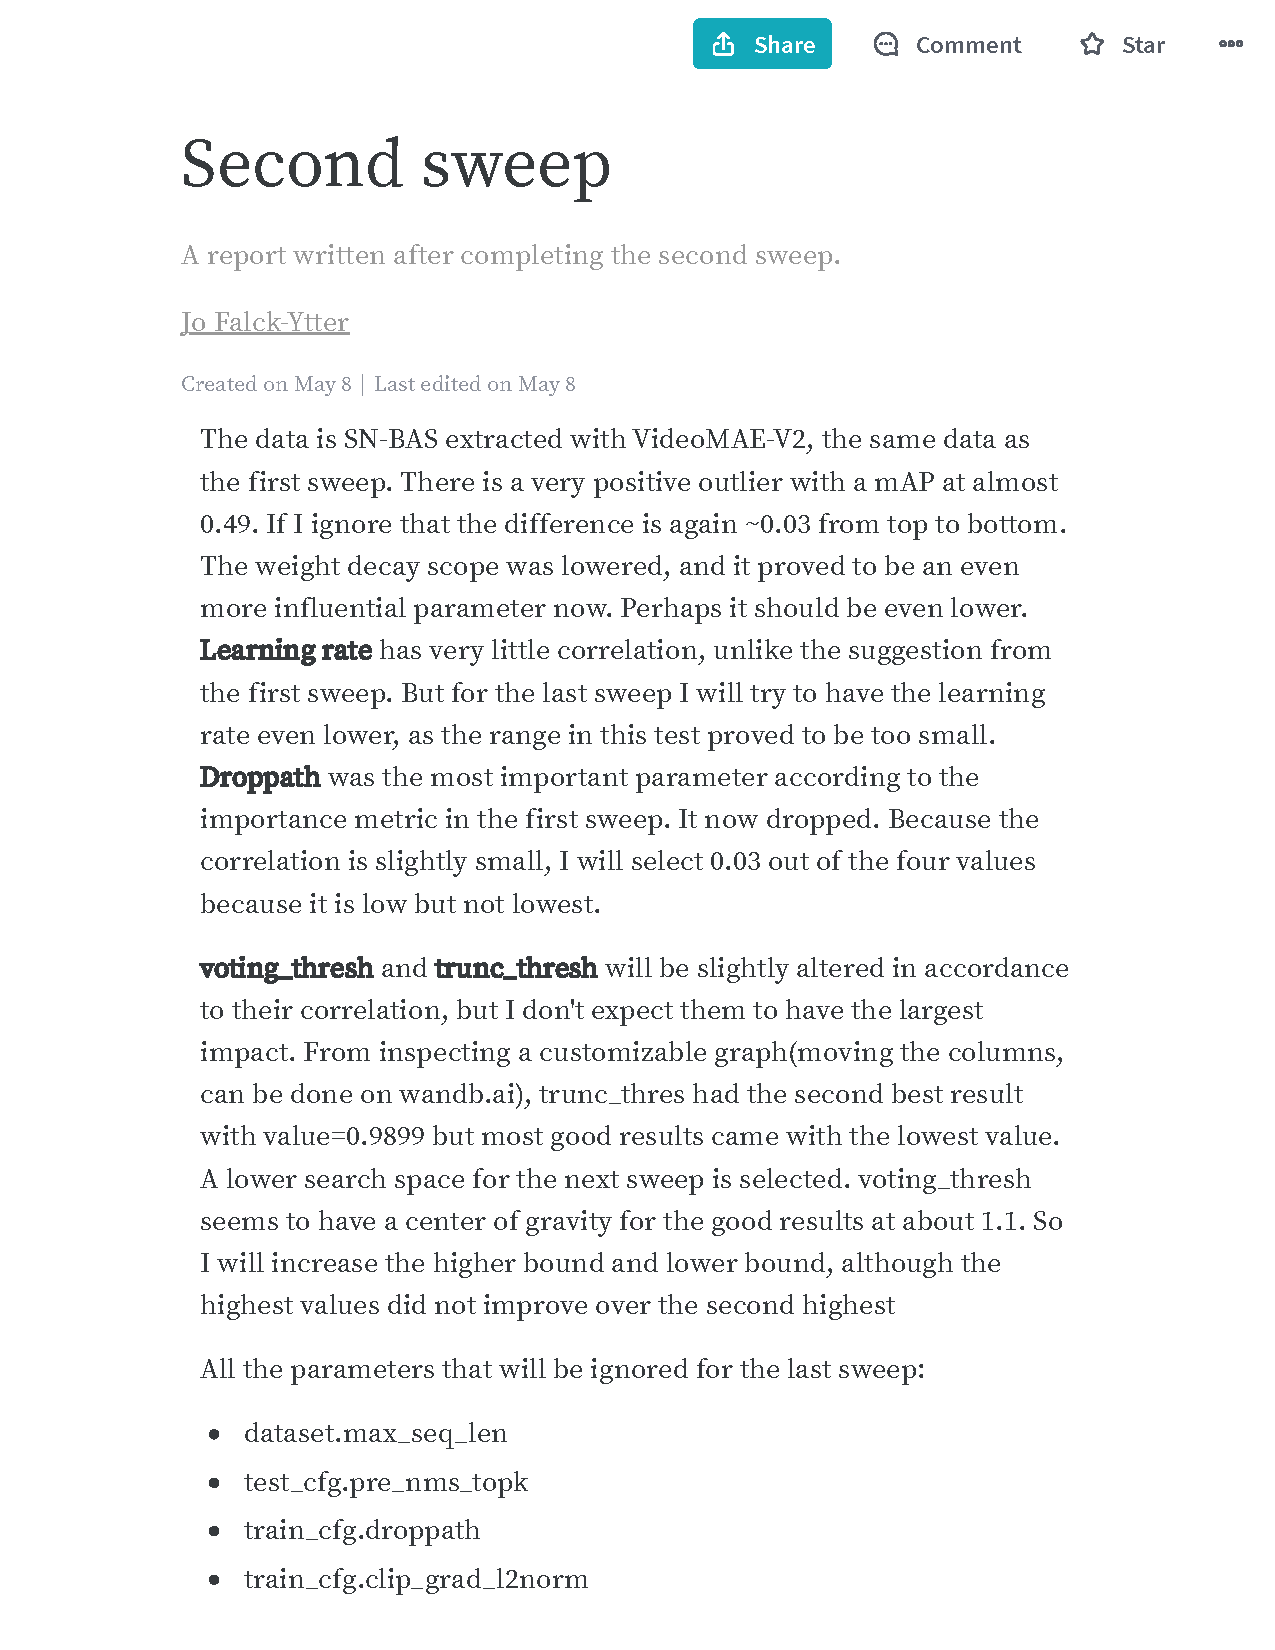
\includepdf[pages=-]{appendices/sweep_2.pdf}

\clearpage
\section{Sweep 3}
\label{app:sweep_3}
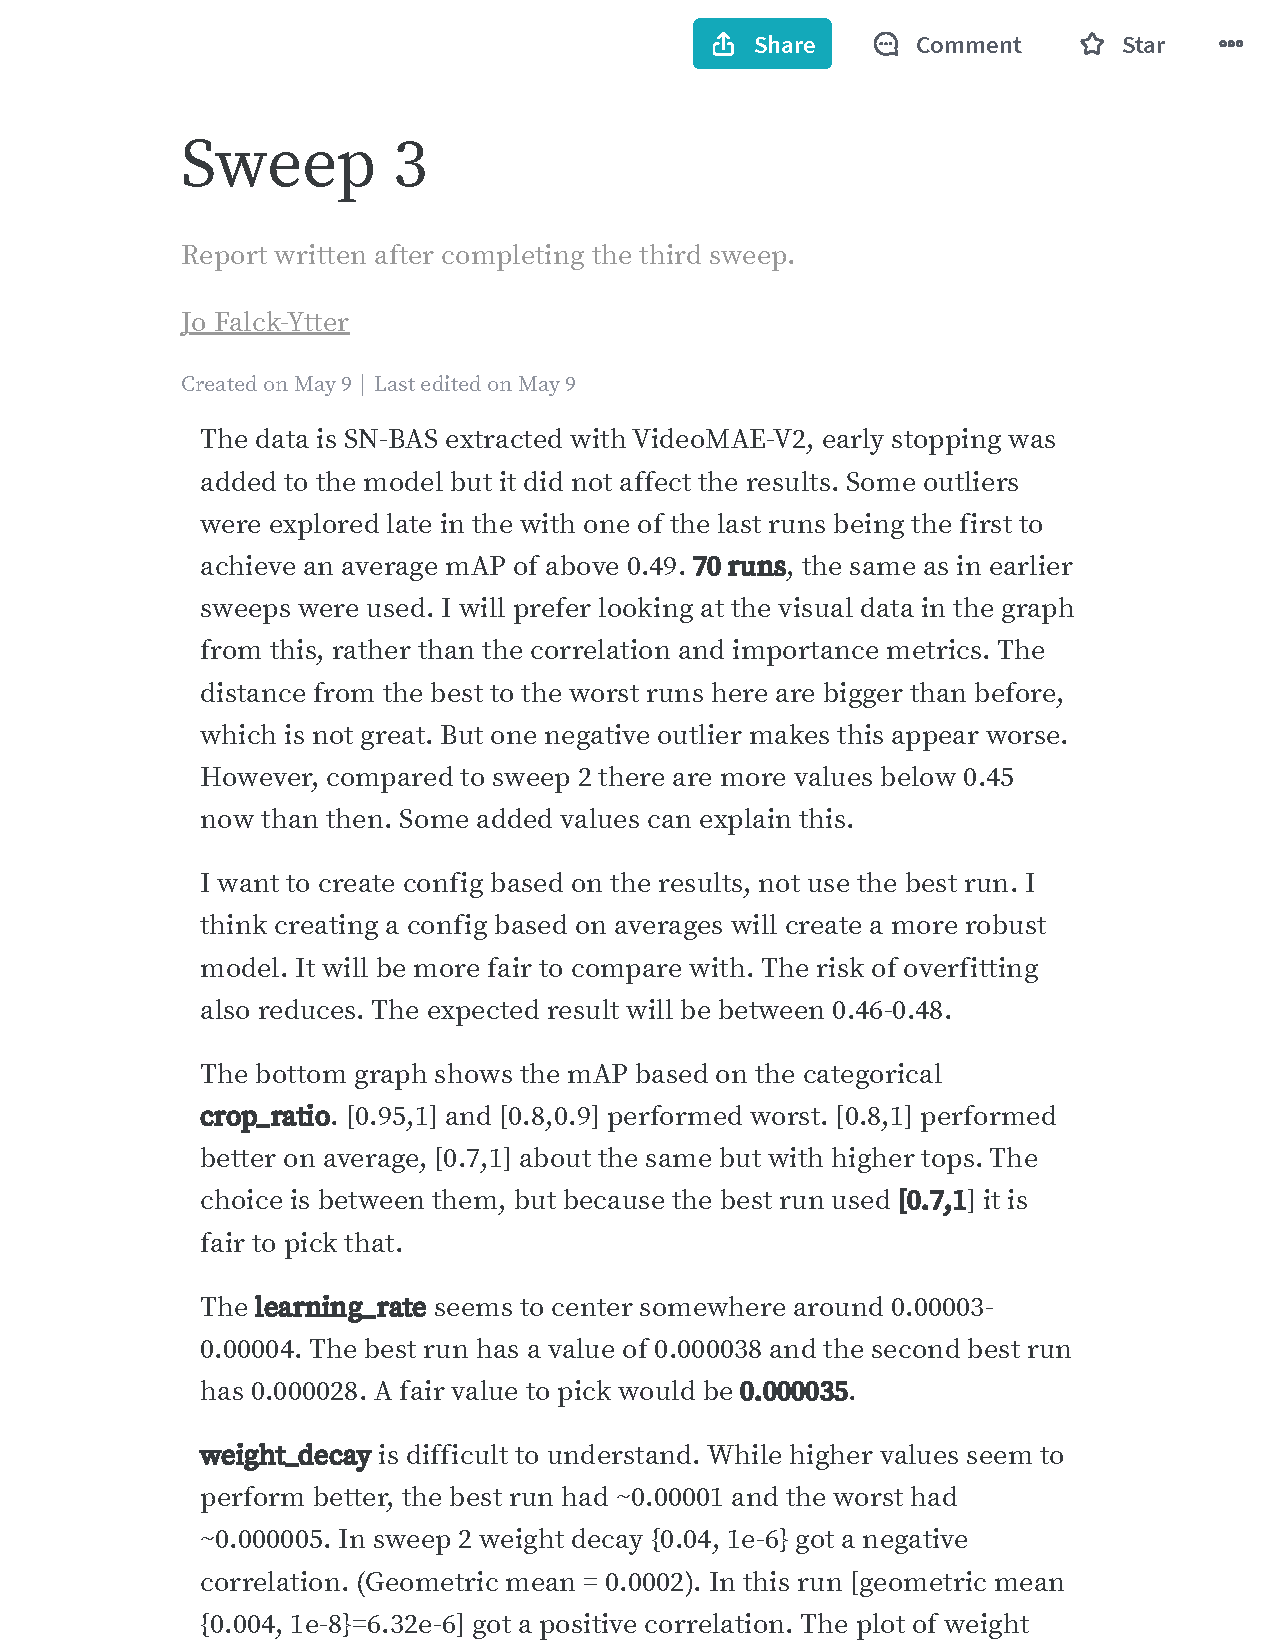
\includepdf[pages=-]{appendices/sweep_3.pdf}


\end{document}
